\AtBeginDocument{%
\begingroup\pagestyle{empty}\raggedright\parindent0pt
{\Formular{\Huge{\titulagemfront{}}}}
\vspace{11.25mm}

\LARGE{\autor}
\vfill
\clearpage

%% Créditos ------------------------------------------------------
\raggedright
\linha{copyright}{\copyrightlivro}
\linhalayout{edição brasileira©}{Hedra \ifdef{\ano}{\ano}{\the\year}}
\linha{tradução©}{\copyrighttraducao}
\linha{organização©}{\copyrightorganizacao}
\linhalayout{coordenação da coleção}{Ieda Lebensztayn}
\linha{prefácio©}{\copyrightintroducao}
\linha{ilustração©}{\copyrightilustracao}\smallskip
\linha{título original}{\titulooriginal}
\linha{edição consultada}{\edicaoconsultada}
\linha{primeira edição}{\primeiraedicao}
\linha{agradecimentos}{\agradecimentos}
\linha{indicação}{\indicacao}\smallskip
\linha{edição}{\edicao}
\linha{coedição}{\coedicao}
\linha{assistência editorial}{\assistencia}
\linha{revisão}{\revisao}
\linha{preparação}{\preparacao}
\linha{iconografia}{\iconografia}
\linhalayout{capa e projeto gráfico}{Lucas Kröeff}
%\linha{capa}{\capa}
\linha{imagem da capa}{\imagemcapa}\smallskip
\linha{ISBN}{\ISBN}\smallskip
\begingroup\tiny
\ifdef{\conselho}{\conselho}{\relax}
\par\endgroup\bigskip

\begingroup \tiny

\textit{Grafia atualizada segundo o Acordo Ortográfico da Língua\\
Portuguesa de 1990, em vigor no Brasil desde 2009.}\\


\vfill\textit{Direitos reservados em l\'ingua\\ portuguesa somente para o Brasil}\\\medskip

%
\textsc{editora hedra ltda.}\\
R.~Fradique Coutinho, 1139 (subsolo)\\
05416--011 São Paulo \textsc{sp} Brasil\\
Telefone/Fax +55 11 3097 8304\\\smallskip
editora@hedra.com.br\\
www.hedra.com.br\\
\bigskip
Foi feito o depósito legal.\\\endgroup
\pagebreak\raggedright
%% Front ---------------------------------------------------------
% Titulo
{\Formular{\Huge{\titulagem}}}
\vspace{11.25mm}

{\LARGE{\autor} \par}%\vspace{1.5ex}}
\vspace{6cm} %9.3cm
\ifdef{\organizador}{{\small {\organizador} (\textit{organização})} \par}{}
\ifdef{\introdutor}{{\small {\introdutor} (\textit{prefácio})} \par}{}
\ifdef{\tradutor}{{\small {\tradutor} (\textit{tradução})}\par}{}\vspace{8.5mm}

{{\footnotesize{} \ifdef{\numeroedicao}{\numeroedicao}{2}ª edição} \par}
%logos
\vfill
\normalsize
\ifdef{\logo}{\IfFileExists{\logo}{\hfill\includegraphics[width=3cm]{\logo}\hfill\logoum{}\\ São Paulo\quad\the\year}}{\logoum\break{} São Paulo\quad\the\year}
%\includegraphics[width=.4\textwidth,trim=0 0 25 0]{logo.jpg}\\\smallskip
\par\clearpage\endgroup
% Resumo -------------------------------------------------------
\begingroup \footnotesize \parindent0pt \parskip 5pt \thispagestyle{empty} \vspace*{-0.1\textheight}\mbox{} \vfill
\baselineskip=.92\baselineskip
\IfFileExists{PRETAS.tex}{
\textbf{Pero Magalhães de Gandavo} tornou"-se um nome tão
obscuro quanto o seu livro. Nem sempre utilizou o último nome, e sabemos que
``gandavo'' é a designação dada a quem nasce em Guantes, Flandres.  Desde a
Biblioteca Lusitana, de Diogo Barbosa Machado, de meados do século
\textsc{xviii}, algumas informações somaram"-se para a invenção histórica da
vida desse nome que teve a posteridade truncada. Diz"-se que fora natural de
Braga, que o pai era flamengo, que foi moço"-de"-câmara de Dom Sebastião, que
trabalhou na Torre do Tombo como copista, que permaneceu alguns anos no Brasil
cuja história escreveu, e que, após a publicação do livro, foi nomeado provedor
da fazenda da cidade da Bahia, cargo que, diz"-se, não exerceu. Teria aberto
uma escola na região entre o Douro e o Minho, onde também casara. A maior parte
das ações e funções institucionais que se lhe atribuem constituía muito do que a
um homem de letras era digno exercer; são provavelmente verossímeis narrativos
do gênero histórico, inventados por tradições biblio"-historiográficas de
escrita de \textit{vidas} de poetas; ou são notícias derivadas desses
verossímeis em vertentes historiográficas do século \textsc{xix}. O mistério que
ronda o desaparecimento de seu livro, aplica"-se a seu estranho sobrenome, que,
sem ascendência nem descendência certas, não se sabe hoje sequer a pronúncia.
       
\textbf{História da província Santa Cruz} (1576) foi lido como ``relato de
viajante'' ou como ``nossa primeira história'', entendido como testemunho de
impressões antigas dos portugueses nas terras d'além"-mar. Contudo, esta
simples história, ou tratado descritivo, da ``costa do Brasil'' teve circulação
muito restrita à época, o que leva a crer que foi recolhida e destruída após sua
impressão, não se sabe bem por quê. Permaneceu praticamente ignorada até 1837,
quando foi reconsiderada na edição e tradução de M.~Henri Ternaux, em Paris; no
século seguinte, foi ainda vertida para o inglês por John B.~Stetson Jr. A
obscuridade do livro nos séculos seguintes à sua publicação é tanto mais
estranha se se tem em vista que, por intermédio de uma elegia e um soneto de
Camões, o livro é dedicado a um varão de armas em carreira promissora nas Índias
portuguesas, tendo sido impresso pela mesma oficina tipográfica que compôs
\textit{Os Lusíadas} (1572), apenas quatro anos mais tarde. Diferente de um
testemunho empírico, o livro é composto conforme a idéia de gênero histórico,
retoricamente regrado, em que o historiador, apoiado pelo aconselhamento ético
da Igreja Católica, tem por fim exaltar, pelo discurso, ações virtuosas de
pessoas de caráter elevado e eventos providenciais. 

\textbf{Ricardo Martins Valle} é doutorando em literatura brasileira pela
\textsc{usp}, e professor de história literária na Universidade Estadual do
sudoeste da Bahia, \textsc{uesb}, campus de Vitória da Conquista.

\textbf{Clara Carolina Santos} é pós"-graduanda do curso de teoria e história
literária da Universidade Estadual do sudoeste da Bahia.  


}{% 
\ifdef{\resumo}{\resumo\par}{}
\ifdef{\sobreobra}{\sobreobra}{}
\ifdef{\sobreautor}{\mbox{}\vspace{4pt}\newline\sobreautor}{}
\ifdef{\sobretradutor}{\newline\sobretradutor}{\relax}
\ifdef{\sobreorganizador}{\vspace{4pt}\newline\sobreorganizador}{\relax}\par}
\thispagestyle{empty} \endgroup
\ifdefvoid{\sobreautor}{}{\pagebreak\ifodd\thepage\paginabranca\fi}
% Sumário -------------------------------------------------------

\sumario{}
%\IfFileExists{INTRO.tex}{
\chapter[Introdução, \emph{por Clara C.~Santos e Ricardo M.~Valle}]{Introdução}
\hedramarkboth{introdução}{Clara C.~Santos e Ricardo M.~Valle}

\begin{flushright}
\textsc{clara c.~santos\\ricardo m.~valle}
\end{flushright}

\section{um livro e um nome}

\noindent{}Impressa em Lisboa, em 1576, na oficina de Antonio Gonçalves, a edição
da \textit{História da província Santa Cruz a que vulgarmente chamamos Brasil
feita por Pero de Magalhães de Gandavo}\footnote{ Nesta edição
seguimos o exemplar pertencente à Biblioteca Nacional de Lisboa da
\textit{História da província Santa Cruz a que vulgarmente chamamos Brasil
feita por Pero de Magalhães de Gandavo}. Lisboa: Officina de Antonio
Gouvea, 1576. Infelizmente a Biblioteca Nacional brasileira não tem
programa de digitalização fotográfica do acervo de obras raras,
dificultando as possibilidades de cotejo, para resolver problemas como
as aparentes irregularidades na página de Aprovação.} é um tratado da terra, isto
é, um laudo documental dos domínios do soberano, com tudo o que neles
houvesse, oferecido neste caso a um vassalo do Rei de Portugal como
louvor dos domínios do mesmo Rei. Pensado até aí, o documento parece
perfeitamente conformado no interior das instituições e regulamentos
institucionais a que então um impresso tinha de submeter"-se. Contudo, o
livro parece ter saído de circulação e o nome do autor praticamente
desaparece por quase dois séculos, principalmente em âmbito português.
A obscuridade do livro nos séculos seguintes à sua publicação é tanto
mais estranha se se tem em vista que, por intermédio de uma elegia e um
soneto de Camões, o livro é dedicado a um varão de armas em carreira
promissora nas Índias portuguesas, tendo sido impresso pela mesma
oficina impressora d'\textit{Os Lusíadas} (1572), que obtivera
alvará de Privilégio real para sair, apenas quatro anos antes.

Falando com rigor, nada efetivamente se sabe a respeito de seu autor,
além de que possivelmente tenha escrito o livro (mais uma ortografia e
alguns outros manuscritos), e de que o tenha feito assinando com este
nome, Pero de Magalhães de Gandavo. Estamos certos, aliás, de que
sabemos até menos do que isso. A designação ``de Gandavo'' 
aparentemente não foi herdada como sobrenome, mas incluído pela pessoa 
do autor e pode ser que para constituir tradição familiar, com vistas a alguma 
fidalguia. Daí se poderia supor também que fosse um imigrado em Portugal 
e que a si passasse a designar pelo patronímico, em verdade ilustríssimo naquele tempo, 
porque sabemos que Gandavo também era Carlos \textsc{v}, nascido em Guantes, 
Flandres, cidade distinguida justamente por esse evento de enorme 
significação para o catolicismo europeu.

Conhecendo os trâmites político"-institucionais a que estava submetido na
hierarquia e valendo"-se dos verossímeis da invenção no gênero
histórico, Barbosa Machado inventou em meados do século 	\textsc{xviii} elementos
da vida do autor. E a recepção moderna tantas vezes apenas acreditou
como efetividade, deixando de lado as possibilidades de pensar, não o
fato particular, que pouco importa, mas as implicações institucionais
supostas a esse quase nada de que se tem notícia, um nome e um
livro.\footnote{ Ver as questões e categorias discutidas por João Adolfo
Hansen em ``Um nome por fazer'', acerca de Gregório de Matos. In: \textit{A sátira e o Engenho}. 
São Paulo/Campinas: Ateliê/Unicamp, 2004, e em “Autor”. In: \textit{José Luís Jobim}. Palavras da
crítica. Rio de Janeiro: Imago, 1992.} Contudo, desde a publicação
francesa, que é do início do século \textsc{xix}, tem"-se reiterado a mesma
informação biográfica, posteriormente acrescentada, ainda que sempre de
poucas notícias.

É verdade que se poderia inventar o verossímil mentiroso de um Gandavo
anônimo, de família portuguesa com ascendência marrana, cristãos"-novos
fugidos da Península Ibérica no tempo de Dona Isabel e Dom Fernando, e
das consequências inclusive jurídicas da ação política dos piedosos e
violentos \textit{reyes católicos de España}, pais de Carlos \textsc{v}. A família
marrana, em processo de limpeza de sangue, serve o Império Católico em
Flandres no tempo do imperador, numa sabidamente lenta ascensão
estamental, por acumulação de dignidades em ofícios letrados. Em 1568,
com a revolução de Orange nos Países Baixos --- com a revisão dos pactos,
as reformas institucionais e as alterações no direito e costume ---, a
família portuguesa de origem judaica, e letrada em âmbito católico, sai
dali para o Brasil, procurando postos subalternos para homens com
algumas letras. Na província portuguesa, Pero de Magalhães (ou como
quer que se tenha chamado) ocupa alguma função anônima na província
portuguesa desta costa do Brasil, onde enriquece e forja documentos
para abreviar a carreira na volta à Europa. Em Lisboa, muito rico e
provavelmente ignorante, ou ao menos cheio de maus acentos no uso da
língua, torna"-se um adulador para conseguir nomeação de escrivão, ou
cronista na Torre do Tombo, seguindo talvez tradição paterna. Paga um
poeta ilustre, um varão de armas sem dinheiro, um impressor e um
historiador para forjar uma obra que lhe conferisse a autoridade de
historiador que lhe ajudaria a receber o cargo tornando"-se mais próximo
de um título de fidalguia. Descoberta a fraude, por irregularidades com
a licença do Paço, desenrola"-se o que é presumível. E com isso, a
memória de seu nome e de seu livro praticamente desaparecem, até que no
tempo da Academia Real de História o livro não fosse reconhecido como
irregular pelas instâncias de chancelaria, passando a ser mencionado,
mas pouco; até que, na Biblioteca  Lusitana, Diogo Barbosa Machado
cumprisse o lugar de bibliógrafo redigindo uma linha de sua vida, aqui
entendida como a espécie do gênero histórico cuja \textit{auctoritas} é
principalmente Plutarco. Com melhor engenho, seria possível inventar
outros particulares verossímeis para a vida de Gandavo, não sendo outra
coisa porém do que a aplicação dos procedimentos da arte de Diogo
Barbosa Machado, cuja notícia a crítica histórica raras vezes deixou de
considerar como o ``pouco que se sabe''.

Pero de Magalhães de Gandavo  tornou"-se um nome tão obscuro quanto o seu
livro. Desde a \textit{Bibliotheca portuguesa} de Barbosa Machado, que é de
meados do século \textsc{xviii}, diz"-se que fora natural de Braga, que o pai era
flamengo, que foi moço"-de"-câmara de Dom Sebastião, que trabalhou na
Torre do Tombo como copista, que permaneceu alguns anos no Brasil cuja
história escreveu, e que, após a publicação do livro, é nomeado
provedor da fazenda da cidade de Salvador, na Bahia, cargo que, diz"-se,
não exerceu. Versado pelo menos nas artes do \textit{trivium} e autor de uma
ortografia portuguesa, teria aberto uma escola na província, na região
entre o Douro e o Minho, onde também casara. A maior parte das ações e
funções institucionais que se lhe atribuíram, contudo, foram atos ou
ofícios que presumivelmente um homem de letras tinha dignidade para
exercer. São provavelmente verossímeis narrativos do gênero histórico,
inventados por tradições biblio e historiográficas de escrita de \textit{vit\ae}
de poetas; ou são notícias derivadas desses verossímeis em vertentes
historiográficas do século \textsc{xix}. O mistério que ronda o desaparecimento
de seu livro, aplica"-se a seu estranho sobrenome, que, sem ascendência
nem descendência certas, não se sabe hoje sequer a sílaba sobre a qual recai o acento.

Desde o século \textsc{xix}, a \textit{História da província Santa Cruz} foi lido como
``relato de viajantes'', ``literatura de informação'' ou como \textit{Nossa
primeira história}, título que recebeu na edição de 1921--1922, entendido
como testemunho de impressões antigas dos portugueses nas terras
d'além"-mar. Contudo, esta simples história, ou tratado
descritivo, da costa do Brasil teve uma circulação muito restrita no
seu século, fazendo parecer que o livro foi recolhido após sua
impressão, não se sabe precisamente por quê. Segundo uma linha de
interpretação da recepção da \textit{História da província Santa Cruz},
sustenta"-se que o livro teria sido recolhido por revelar segredos de
Estado sobre a província portuguesa, como a posição de rios e cidades
da costa do Brasil, segundo o que os historiadores chamaram de
``política do segredo'' de Dom Manuel \textsc{i}.\footnote{ Cf.~Sheila 
Moura Hue e Ronaldo Menegaz.
``Introdução''. In:  \textit{Primeira História do
Brasil. História da província Santa Cruz a que vulgarmente chamamos
Brasil}. Rio de Janeiro: Jorge Zahar, 2004, p.~14.} O certo é que
permaneceu praticamente ignorado até a primeira metade do século \textsc{xix},
quando foi reconsiderado na edição e tradução de M. Henri Ternaux, em
Paris, em 1837; e no século seguinte foi ainda vertido para o inglês
por John B. Stetson Jr., em 1969. No início do século \textsc{xviii}, com o
fomento à divulgação das navegações e feitos portugueses pelas
Academias de História no reinado de Dom João \textsc{v}, o opúsculo de Gandavo
consta dos documentos então exumados pela Real Academia, o que se prova
com a ocorrência secundária no Bluteau e logo na Biblioteca de Diogo
Barbosa Machado, em meados do século \textsc{xviii}, fazendo a essa regra raras
exceções, sendo mantido ainda em ampla obscuridade até a edição
francesa na primeira metade do século \textsc{xix}.

Diferente de um testemunho empírico, o livro é composto como gênero
histórico, retoricamente regrado, em que o historiador, apoiado pelo
aconselhamento ético da Igreja Católica, tem por últimos fins exaltar,
pelo discurso, ações virtuosas de pessoas de caráter elevado e eventos
providenciais; levar adiante a fama do monarca e dos homens de armas a
quem é dedicado; e legitimar sua autoridade e senhorio, com direito de
propriedade, sobre terras, rios, espécies animais e vegetais, pedras,
metais etc., que se podem usar e dispor como próprios, conforme aos
grandes axiomas e aos anátemas que regulavam estas disposições na forma
das leis civis e eclesiásticas. Estes fins deveriam atingir"-se pela
aplicação de procedimentos e lugares retóricos, entre os quais a
amplificação da beleza, utilidade, fertilidade, abundância etc., como
louvor dos novos domínios da Cristandade portuguesa. Neste sentido,
relata, ou historia, as particularidades da terra e de sua conquista
como louvor do feito português, visando à perpetuação da empresa
marítima lusitana a partir de uma narrativa que segue principalmente os
modelos preceptivos de Menandro, retor, e Plínio, o Velho, entre outras
autoridades de escrita histórica.

\section{a história como\break demonstração da sujeição}

Seja como for, num tempo em que a conservação da fama do nome,
transmitido pela família, é fundamental para a aquisição de favores,
dignidades, benefícios de estado, e sabendo ainda que o livro impresso
era instrumento de perpetuação de nomes e dignidades institucionais, é
sem dúvida extraordinário um tal desaparecimento. Conforme à aplicação
da tópica da perenidade das letras, o ``Prólogo ao
Leitor'' (parte do exórdio que se dirige ao auditório
retoricamente constituído como um gênero de homens ao menos letrados em
boas letras), o autor da \textit{História da província} repõe que
``a escritura seja vida da memória, e a memória uma
semelhança da imortalidade a que todos devemos aspirar''.

Como não interessa aqui encontrar a afirmação da verdade particular da
História, o provável, ou verossímil, infortúnio de Gandavo permite"-nos
pensar procedimentos de representação institucional que, como demonstra
João Adolfo Hansen, estão muito diretamente ligados às práticas
letradas, entre as quais a história e a poesia, como a teologia moral e
a jurisprudência etc. conforme os ofícios em questão:

\begin{hedraquote}
Na fronteira das categorias do imaginário social mais amplo e das
categorias dos grupos cultivados, situava"-se então a imagem do
sábio"-letrado, padre ou funcionário, muitas vezes poeta. A imagem era
equívoca, pois nela convergiam as representações do letrado"-artesão,
escrevente que simplesmente repetia a tradição, fazendo cópias
manuscritas de textos, e do letrado sábio, que reinventava em novas
ocasiões. [\ldots{}] As práticas dos letrados portugueses não se
autonomizavam da hierarquia, e, não sendo mais escrivães medievais, mas
também não sendo escritores, no sentido iluminista dado ao termo a
partir da segunda metade do século \textsc{xviii}, eles se identificavam com a
imagem social da profissão que exerciam e essa era, obviamente,
profissão subordinada ao poder real.\footnote{ João Adolfo Hansen,
``Fênix renascida \& Postilhão de Apolo''. In: \textit{Poesia seiscentista}. São Paulo: Hedra, 2002.} 
\end{hedraquote}

Com efeito, antes de imprimir sua \textit{História da província Santa Cruz},
Gandavo dedicou mais de um tratado da terra aos principais do reino,
declarando fidelidade no uso que faz das letras. Trata"-se do manuscrito
intitulado \textit{Tratado da terra do Brasil no qual se contem a informação
das cousas que há nestas partes feito por Pº de magalhães},\footnote{ Para 
um cotejo que explicita as diferenças do texto
do \textit{Tratado da terra do Brasil} e da \textit{História da província Santa Cruz},
ver notas à edição de Sheila Moura Hue e Ronaldo Menegaz, op.~cit. Vale
lembrar, porém, que o \textit{Tratado} manuscrito e a \textit{História} impressa são
dois textos, no todo, diversos.} também pertencente à Biblioteca
Nacional de Lisboa, que os disponibiliza no Acervo Digital. A versão
impressa é dedicada a dom Lionis Pereira, varão de armas de altura
ainda mediana na vassalagem portuguesa, e de quem sabemos que foi
capitão em Malaca, em 1564, e em Ceuta, em 1580, tendo passado
certamente por outros postos que acumularam mérito oficial para que de
tão longe passasse a tão perto, o que era evidentemente uma melhora no
interior do estamento de que participava. O manuscrito, por sua vez, é
dedicado ao Príncipe Cardeal"-Infante dom Henriques, o futuro regente
interino do reino e províncias portugueses, entre o desaparecimento de
Dom Sebastião, em 1578, e a ascensão de Filipe \textsc{ii} de Espanha, em 1580.
Na posição de um homem de letras, que demonstra sua fidelidade e
aptidão, o manuscrito assinado por Pero de magalhães (com minúscula,
como quase sempre assinava a gente sem fidalguia ou alguma distinção no
século \textsc{xvi} em Portugal) dirige"-se a um dos dois maiores postos do reino
num documento sem data. Esse manuscrito também não leva o obscuro
sobrenome supostamente paterno, Gandavo, e que só mesmo o século \textsc{xix}
francês elevou a alguma fama.

Neste ``sumário da terra do Brasil'' --- como é
designado pelo autor ---, o vassalo alega já ter feito e dedicado uma
cópia do seu tratado a Dom Sebastião, passando agora a fazê"-lo ao seu
tio, sucessor imediato, numa carta dedicatória ``Ao mui
alto e sereníssimo Príncipe dom Henrique Cardeal Infante de Portugal'':
\begin{hedraquote}
Posto que os dias passados apresentei outro sumário da terra do Brasil a
el"-Rei nosso senhor, foi por cumprir primeiro com esta obrigação de
vassalo que todos devemos a nosso Rei: e por esta razão me pareceu
cousa mui necessária (muito Alto e Sereníssimo señor) oferecer também
este a \textsc{v.a.} a quem se devem referir os louvores e acrescentamento das
terras que nestes Reinos florecem: pois sempre desejou tanto
aumentá"-las e conservar seus súditos e vassalos em paz.
\end{hedraquote}

Dada a altura elevadíssima das pessoas a quem o pequeno vassalo se
dirigia, é muito provável que seja verdadeira a informação acerca da
existência de outra versão manuscrita anterior à que conhecemos. A
informação, porém, aqui interessa para lembrar que a cópia conhecida,
tendo sido dedicada ao Cardeal"-Infante Dom Henriques, não poderia ser
considerada uma primeira redação ou esboço, como se o manuscrito
necessariamente estivesse destinado a receber letra de forma. Talvez
seja apenas uma outra espécie de documento. De qualquer modo, bastante
diferente de um rascunho, as cópias do \textit{Tratado da terra do Brasil}
cumprem certamente um papel institucional, por meio de uma
representação, ou ostentação, de fidelidade à soberania das ordens
superiores que governam o Estado; trata"-se de uma declaração de
reconhecimento, por parte do súdito, da necessidade sagrada da
hierarquia dos homens. Uma vez então que seja mais seguramente o
cumprimento de um dever de ``subdito e vassallo'' e ainda a demonstração de sua (humilde)
utilidade em ofícios que requeiram boas letras, o manuscrito não tem
uma natureza mais verídica no relato, ou história, da terra, nem
significa uma observação empírica mais autêntica, como foi interpretado
pela crítica historiográfica no século \textsc{xx} que procurou ler esses
documentos como ``História do Brasil'', ``literatura de informação'' ou
``de viajantes'', sem considerar muitas vezes os âmbitos institucionais, 
as disposições jurídicas e os procedimentos discursivos que estavam supostos.

\section{o poder constituído das mesas censórias}

Na segunda metade do século \textsc{xvi}, as aprovações do Ordinário, da
Inquisição e do Paço atestavam a verdade da instrução que o livro
continha, segundo as Leis católicas e do Império português, que em
grande medida são extensão umas das outras. Sejam livros úteis, como os
de Lei e os Sagrados, sejam os de recreação, como os de história ou
poesia,\footnote{ Empregamos aqui a classificação que se lê nas páginas
iniciais do \textit{Corte na aldeia} (1619), de Rodrigues Lobo, que inclui como
livros de recreação, de um lado, os de histórias fingidas, compreendendo
as cavalarias de \textit{res ficta}, isto é, de matérias fingidas, análogos neste
sentido de muitos gêneros da poesia, e de outro lado os de história
verdadeira, como podem ser pensadas as crônicas, décadas, tratados da
terra, etc. (Cf.~\textit{Obras políticas morais e métricas do insigne Portugues
Francisco Rodrigues Lobo. Natural da Cidade de Leyria. Nesta última
impressão novamente correcta, e postas por ordem. Offerecidas à
Magestade sempre augusta do Sereníssimo Rey de Portugal. D. João \textsc{v},
nosso senhor}. Lisboa Oriental: Na Officina Ferreyriana. 1723;
pp.~3--4.)} somente a concórdia entre as mesas conferia a completa
autorização para a impressão e circulação do livro, cruzando"-o com a
tradição das autoridades e axiomas de doutrina ou instrução verdadeira;
entendendo por tradição aqui o sentido com que o Concílio de Trento
distiguia boas e más tradições discursivas, tendo em vista que 

\begin{hedraquote}
esta verdade, e disciplina se contém em livros escritos, e sem escritos,
nas Tradições, que recebidas pelos Apóstolos da boca de Cristo, ou
ditadas pelo Espírito Santo, dos mesmos Apóstolos como de mão em mão
chegaram até nós; seguindo o exemplo dos Padres Ortodoxos [\ldots{}]; como
ditadas pela boca de Cristo, ou pelo Espírito Santo, e por uma
contínua sucessão, conservadas na Igreja Católica [\ldots{}].\footnote{ Sessão 
\textsc{iv}, do Concílio de Trento. Citamos pela edição bilíngue do
século 	\textsc{xviii}: \textit{O sacrosanto, e ecumenico Concilio de Trento Em Latim, e
Portuguez}. Trad. João Baptista Reycend. Lisboa: Na officina Patriarcal
de Luiz Ameno, 1781, Tomo \textsc{i}, p.~55.}
\end{hedraquote}

Como ficou dito, os destinatários das duas versões manuscritas (a
primeira delas apenas hipotética) são as duas mais poderosas
representações políticas daquelas décadas. Um é o jovem rei, que tem
representação primordialmente jurídico"-militar --- e, no caso particular
de Dom Sebastião, sobretudo militar e piedosa, segundo a invenção da
fama do nome na instituição histórica, cujo fim, entre as funções
bibliotecárias do reino desde antes de Fernão Lopes, era conferir
legitimidade à autoridade das potestades instituídas no presente.
Independentemente da feição particular da representação tipológica que
assume, o rei devia ser reconhecido como autoridade que reúne a
soberania sobre a totalidade das potestades, ofícios, artes e demais
serviços do reino, uma vez que seja monarca. Já o destinatário do
\textit{Tratado da terra do Brasil} que efetivamente nós podemos ler é o tio do
mesmo monarca, o velho Inquisidor"-mor, Cardeal dominicano, Dom
Henriques, que tinha autoridade direta sobre as três instâncias de
censura: do Ordinário, da Inquisição e do Paço. A mesa do Ordinário dá
vista e aprovação, ou a nega, normalmente pela autoridade de um doutor
em leis ou teologia escolhido entre os bispos da diocese para a função
\textit{ad hoc} de vedor ou qualificador. Como junta ou conselho episcopal do
reino, os membros do Ordinário estão necessariamente sob a autoridade
do Cardeal"-Infante, ainda mais quando o príncipe"-sacerdote é o próprio
Inquisidor do Paço. Além disso, sabemos que mesmo o Conselho Geral da
Inquisição havia sido instalado em Portugal sob a ação do mesmo
Cardeal"-Infante, feito Inquisidor"-mor por seu irmão, Dom João \textsc{iii},
décadas antes. 

Segundo o Concílio de Trento, os livros de matérias sagradas e, por
necessidade, toda matéria sagrada contida em livros de qualquer
espécie, deveriam ser conferidos, sob pena, com o ``verdadeiro sentido, 
e interpretação das Escrituras'', isto é, ``o unânime consenso
dos padres''. Assim, decreta que 

\begin{hedraquote}
a ninguém é lícito imprimir, nem mandar imprimir Livros alguns de
matérias sagradas sem nome do Autor, nem vendê"-los daqui em diante;
nem também tê"-los em seu poder, sem serem primeiro examinados, e
aprovados pelo Ordinário, sob pena de excomunhão [\ldots{}]. E se forem
Regulares (os Autores) além deste exame, e aprovação, estarão
obrigados a impetrar também Licença dos seus Superiores, sendo por
eles examinados os livros, na forma das suas Constituições.\footnote{ Idem, ibidem. pp.~61--63.}
\end{hedraquote}

Além de valer para qualquer documento manuscrito, as penas se estendiam
aos impressores, vendedores, possuidores e leitores da obra que
ilegalmente fosse posta em circulação. A censura do Ordinário em
Portugal, como na Espanha, era já exercida antes do Concílio --- e como
mostra a própria folha de ``Aprovação'' desta
\emph{História da província Santa Cruz} ---, a licença do Ordinário
subordinava"-se à petição do Conselho Geral da Inquisição. E assim como
os clérigos regulares deveriam ter ainda a permissão dos superiores da
Ordem a que pertencessem, os súditos deveriam ter a aprovação de seu
rei, o que em Portugal se fazia pela censura do Paço.

No livro de Gandavo em particular, a Licença do Conselho Geral do Santo
Ofício da Inquisição acredita o testemunho do vedor de livros do
Ordinário; tudo feito no interior de rígidas praxes, instituídas e
acostumadas por décadas. A aprovação do Santo Ofício apenas ratifica,
aparentemente sem exame, a informação de que o livro não continha coisa
que se pudesse considerar inimiga da santa fé e do bom costume
cristãos, não colocando em suspeição nem os mistérios nem os usos da
fé, sempre segundo o costume apostólico romano e terminantemente
revogadas pelo Concílio quaisquer tradições de opinião contrária ou
fundadas na própria prudência e livre inteligência das coisas sagradas.
Segundo o Decreto aposto à mesma Sessão do Concílio:
\begin{hedraquote}
para refrear engenhos petulantes, determina: que ninguém confiado na sua
prudência, em matérias de Fé, e costumes, e edificação da Doutrina
Cristã, torça a sagrada Escritura para os seus conceitos particulares,
contra aquele sentido que abraçou, e abraça a Santa Madre Igreja, a
quem pertence julgar o verdadeiro sentido e interpretação das
Escrituras; nem se atreva a interpretar a mesma Escritura contra o
unânime consenso dos Padres; ainda que estas interpretações nunca hajam
de se dar a luz. Os que a isto contravierem, sejam pelos Ordinários
declarados, e castigados com as penas estabelecidas em
direito.\footnote{ Idem, ibidem. pp.~59--61.}
\end{hedraquote}

O livro de Gandavo aparentemente não se choca com o Decreto, mas não
deixa de ser notável que, no exemplar que transcrevemos, pertencente à
Biblioteca Nacional de Lisboa, que o publica digitalmente, a caixa de
texto da licença do Paço apresenta recuo maior de ambos os lados e o
alinhamento horizontal é ligeiramente pendente à esquerda, o que pode
indicar que a inserção foi feita posteriormente. A hipótese talvez
fosse excessiva, não houvesse notícia pela Biblioteca John Carter Brown
de que há exemplares com e sem a terceira caixa de texto.\footnote{ A
informação é de Rubens Borba de Moraes, que compara os exemplares da
Biblioteca \textsc{jcb} com o exemplar da Biblioteca Nacional do Rio de Janeiro.
Não pudemos, contudo, auferir a autenticidade da informação (Cf.
\textit{Bibliografia brasileira do período colonial}. São Paulo: Instituto de
Estudos Brasileiros, \textsc{usp}, 1969). A pesquisadora Valéria Gauz, que
trabalhou tanto na Biblioteca Nacional quanto na John Carter Brown,
menciona esse dado no texto ``Materialidade de livros -- \textsc{ii}'', disponível no site da \textsc{info}\textit{home}. 
O acervo da Biblioteca Nacional brasileira, contudo, não é
disponibilizado digitalmente.} Tudo isso, que é nada, na mera hipótese
sobre o particular, apenas permite insinuar problemas na tese que
explica diretamente o desaparecimento do livro por violação de segredo
de Estado, ainda que a hipótese continue válida. É mesmo muito
plausível que o desaparecimento do livro tenha sido causado por razão
de Estado, mesmo porque o acaso raras vezes é tão violento quanto as
instituições normativas. Esses particulares conhecíveis não teriam
maior interesse, se o manuscrito conservado não fosse dedicado
justamente à altíssima autoridade censória do reino, ao mesmo tempo que
sua versão impressa, recomendada por Camões, parece ter sido destruída
por força estatal, do contrário não teria sido elidido na quase
totalidade de seus exemplares. À aparente irregularidade da página de
``Aprovação'', se se confirmar que há volumes
sem a terceira licença, que é a do Paço, podem"-se fazer suposições
inúmeras que talvez tenham \mbox{interesse se} forem pensadas a partir dos
mecanismos institucionais e discursivos que constituem historicamente
essas relações de poder.

\section{aos empobrecidos do reino}

Ainda na Dedicatória do \textit{Tratado da terra}, Pero de Magalhães, de
Gandavo, afeta modéstia, como tem de ser, para produzir retoricamente
benevolência no destinatário; para isso, elogia a utilidade da matéria
do seu tratado, com o que se quer demonstrar também a utilidade do
serviço do vassalo fiel em ofícios de letras:

\begin{hedraquote}
achei que não se podia dum fraco homem esperar maior serviço (ainda que
tal não pareça) que lançar mão desta informação da terra do Brasil
%Jorge: empreendeu
(cousa que até agora não empreendeu pessoa alguma) para que nestes Reinos
se divulgue sua fertilidade e provoque a muitas pessoas pobres que se
vão viver a esta província, que nisso consiste a felicidade e aumento dela.
\end{hedraquote}

Duas vezes repetida nesta carta dedicatória ao Cardeal"-Infante, bem como
no ``Prólogo ao Leitor'' da \textit{História da província Santa Cruz}, 
a recomendação da costa do Brasil para os
portugueses que estejam em pobreza na pátria é também empregada no
exórdio do livro impresso, sempre como argumento da utilidade do
sumário da terra, bem como dos serviços de quem o escreve, exercendo,
pois, dupla função, ao mesmo tempo retórica e política. Deveríamos
talvez supor que, sendo no mínimo gente de letras os seus leitores, a
condição de ``pobres e desamparados'' não designa o que as sinuosas 
classificações econômicas reconheceriam como
\textsc{c, d ou e}, nos sistemas de regulação por poder aquisitivo. Num corpo
político constituído por estados, ou ordens civis, os empobrecidos eram
mais provavelmente gente de baixa fidalguia, militares e letrados em
geral, cristãos"-velhos de ofício livre, possivelmente até
cristãos"-novos em processo de limpeza de sangue e lenta ascensão na
fidelidade institucional. A plebe mais baixa até estava implicada nesta
solução que o encarecimento da matéria do livro oferecia para a pobreza
dos pobres, mas estava suposta apenas como criadagem e companhia de
gente mediana, ou clientela de gente semiarruinada, ou ainda oficiais
mecânicos, mercenários, negociantes, exilados ou bandidos fugidos,
todos os pobres que por suposto também viriam, mas aos quais o livro de
Gandavo dificilmente se destinava, a não ser por exceção.

Tendo em vista os mecanismos da imensa hierarquia do império português,
o autor supõe demonstrar a utilidade de seu discurso colocando"-o a
serviço do necessário encorajamento às carreiras militares, jurídicas,
fiscais etc., na costa do Brasil, ainda designada província Santa
Cruz. Dirige"-se, portanto, à gente de carreira, isto é, gente
minimamente remediada para as instituições civis, educadas para o
preenchimento de funções direta ou indiretamente administrativas na
povoação e defesa dos novos domínios do reino, conforme o caso, mas
acometida por toda sorte de infortúnio que não fosse causado por crime.
Em outro uso, Antonio de Guevara, grande autoridade letrada do Império
Habsburgo no século \textsc{xvi}, avisava dos perigos da corte se dirigindo a
homens dignos de alguma distinção mas também empobrecidos por má
fortuna, recomendando os benefícios da recolha à província.\footnote{ Antonio 
de Guevara. \textit{Menosprecio de corte y alabanza de aldea} (1539).
Edición y notas de M. Martínez de Burgos. Madrid: Espasa"-Calpe, 1942.}
As diferenças entre os argumentos do elogio da aldeia, de Guevara, e da
recomendação feita nos exórdios dos breves tratados históricos da
terra, de Gandavo, são proporcionais aos decoros específicos, próprios
ao assunto e finalidade de cada livro. Em ambos os casos (e muitos
outros poderiam ser referidos), recomenda"-se o afastamento da corte
como um caminho difícil mas seguro para o exercício das boas virtudes
cristãs ou dos úteis serviços da fidelidade monárquica, com promessas
de prêmios nesta e na outra vida. Preenchendo o lugar retórico da
captação da benevolência --- no caso, pela defesa  e encarecimento da
matéria tratada ---, a recomendação de Gandavo, ainda que tenha
significação política, não precisaria ser lida com mais graves
consequências, ao menos não para que se pensem hipóteses sobre a origem
da pobreza do Brasil. A constituição política que está suposta nesta
exortação às carreiras do Novo Mundo ``dá sentido'', e talvez maior interesse, 
à descrição dos mantimentos da terra, bem como da barbárie dos nativos. 
Mas o sentido só ``é dado'' a nós que lemos o texto hoje, com outros hábitos de leitura. 
No seu tempo, o sentido já estava dado, salvo dissensos, que sempre existiram 
apesar dos sistemas de controle dos atos discursivos. 

``Primeiramente tratarei da planta e raiz de que os
moradores fazem seus mantimentos que lá comem em lugar de
pão.'' Assim começa o passo em que tratará da mandioca, de
que se extrai a farinha cuja técnica de uso Gandavo relata no
``Capítulo \textsc{v} --- Das plantas, mantimentos, e frutas que há
nesta província''. A mandioca é o análogo do trigo,
aproximado da raiz por sua finalidade, segundo modos de classificação
reconhecidos pelo português. Conforme a redação do \textit{Tratado} manuscrito:
\begin{hedraquote}
Nestas partes do Brasil não semeiam trigo nem se dá outro mantimento algum
deste Reino; o que lá se come em lugar de pão é farinha de pão: esta
se faz da raiz duma pranta que se chama mandioca, a qual é como inhame.
\end{hedraquote}

Como se dispõe a falar ``principalmente daquelas [plantas,
frutas e ervas], de cuja virtude e fruto participam os
Portugueses'' [Capítulo \textsc{v}], sempre segundo preceituam os
antigos retores do gênero histórico, a esta preeminência está suposto
que de trigo se faz pão, que é base da constituição alimentar do corpo
físico do vassalo cristão e base material para a consagração do Corpo
espiritual da comunidade de Cristo na eucaristia. Não por acaso a
mandioca, seu análogo, é o primeiro mantimento referido tanto na
\textit{História da província}, quanto no manuscrito do \textit{Tratado} da terra. Por
essa razão, também nas crônicas, tratados e histórias desta mesma
terra, escritos em português posteriormente, a mesma planta e seus usos
terão similar descrição e preeminência, sendo muitas vezes reiterada
sua analogia com o trigo, mesmo que o texto de Gandavo não tenha se
tornado fonte para a maior parte delas, devido a seu desaparecimento. O
caso da mandioca evidencia, portanto, que as descrições da fauna,
flora, costumes etc., eram redigidas segundo procedimentos
convencionais, orientados retórica, política e teologicamente.

O discurso de aconselhamento aos empobrecidos da pátria demonstra a
utilidade da matéria inventada, e por isso mesmo ocupa lugar
preeminente na escolha das matérias particulares de que tratará --- como
a abundância de mantimento, de água, de terra, de caça etc., e a
promessa de muitas pedras e metais ---, e que hoje se leem como elenco de
curiosidades especiosas da terra, por uma espécie de contaminação
turística de nossos tempos tristes, como outrora havia sido argumento
de ``porque me ufano'' de ser brasileiro, nas leituras românticas e
modernistas do texto, muitas vezes associadas institucionalmente a
jubileus comemorativos, como os cem anos da Independência, e aos
eventos bibliográficos, ou já editoriais, a eles ligados, direta ou
indiretamente. O aconselhamento aos empobrecidos não se contradiz pela
horrenda descrição dos índios e seus perigos, que se leem nas
terríveis, e exemplares, cenas de antropofagia que Gandavo produz na
última terça parte do livro. A exortação à carreira no ultramar não
seria de modo verossímil promissora em demonstração de virtude e heroísmo,
não houvesse obstáculos que a fé e a obediência do súdito deveriam
vencer para efetivamente melhorar de vida, isto é, adquirir dignidade
no interior da efetividade da instituição armada do Estado, e suas
demandas.

\section{gentilidade e justa dominação}

As terras que louvando se descrevem são entendidas como territórios
desertos, ou seja, ainda largamente desocupados de convívio civil.
Segundo o consenso dos padres e maiores potestades da Terra na
hierarquia do cristianismo romano, os naturais da terra viviam pouco
acima dos animais, isto entendido aristotelicamente como uso restrito,
precário ou torpe das potências superiores da alma. Em alguns casos,
como parece ser o de Gandavo, em geral a gentilidade da terra é
representada como incivil, algumas de suas nações são descritas, por
seus costumes, como bárbaras ou quase bestas, isso entendido como
deformidade da alma, causada pelos maus usos por séculos acostumados,
como se dizia.
\begin{hedraquote}
Já que tratamos da terra, e das coisas que nela foram criadas para o
homem, razão parece que demos aqui notícia dos naturais dela; a qual
posto que não seja de todos em geral, será especialmente daqueles que
habitam pela costa, e em partes pelo sertão dentro muitas léguas com
que temos comunicação. Os quais ainda que estejam divisos, e haja entre
eles diversos nomes de nações, todavia na semelhança, condição,
costumes, e ritos gentílicos todos são uns. E se em alguma maneira diferem
nesta parte, é tão pouco, que se não pode fazer caso disso, nem
particularizar cousas semelhantes, entre outras mais notáveis [\ldots{}]. 
Pela maior parte são bem dispostos, rijos e de boa estatura. Gente mui
esforçada e que estima pouco morrer, temerária na guerra e de muito
pouca consideração. São desagradecidos em grã maneira, e mui desumanos
e cruéis inclinados a pelejar e vingativos por extremo. Vivem todos mui
descansados sem terem outro pensamentos, senão de comer, beber, e matar
gente [\ldots{}].  São mui desonestos e dados à sensualidade, e assim se
entregam aos vícios como se neles não houvera razão de homens. Ainda
que todavia em seu ajuntamento os machos com as fêmeas tem o devido
resguardo, e nisto mostram ter alguma vergonha.

A língua de que usam,
toda pela costa é uma: ainda que em certos vocábulos difere em algumas
partes [\ldots{}]. Alguns vocábulos há nela de que não usam senão as fêmeas  e outros
que não o servem senão pera os machos. Carece de três letras, convém a
saber, não se acha nela, \textit{f}, nem, \textit{l}, nem, \textit{r} cousa digna de espanto, porque
assim não têm Fé, nem Lei, nem Rei: e desta maneira vivem
desordenadamente sem terem além disto conta, nem peso, nem medido.\footnote{ Página~\pageref{feleirei}.}
\end{hedraquote}

De saída, logo na introdução do novo assunto --- isto é, as coisas
relativas às gentes, sobre as quais discorrerá entre os Capítulos \textsc{x} e
\textsc{xiii} ---, a descrição exemplar da barbárie supõe indicativamente o modelo
teológico sobre o qual se assenta; por suposto, implica também o
reconhecimento da validade da alma imortal aristotélica e, por essa
razão, representa o índio como um ser humano, conforme a bula papal e o
Concílio de Trento, mas conduzido à animalidade pela destituição ou
descontrole das potências eternas da alma, ``como se neles
não houvera razão de homens'', a que se faz a ressalva de
que no coito seu costume demonstra pudor, vestígio de alma. Na
perspectiva católica que articula a descrição histórica do natural da
terra, só a louca fantasia e as voracidades do corpo poderiam, neste
sentido, governar os homens que por exemplo comessem o semelhante, e
mesmo o familiar, por costume e, pior, respeitante a leis. Em alguns
casos como o dos Aimorés, são considerados bestas, mas contra a
natureza, portanto por impiedade deliberada deles mesmos, assim
tornados, em termos católicos, pelo mau uso do livre"-arbítrio, que
levando a más práticas depois acostumadas por más tradições, segundo
uma interpretação que considere o texto de Gandavo como ortodoxo, do
ponto de vista dos direitos.

Numa interpretação diferente desta, João Adolfo Hansen entende a
descrição de Gandavo como adoção da tese herética sobre o gentio, que
foi opinião comum entre colonos portugueses no Brasil, partidários da
escravização indígena. Em ``A servidão natural do selvagem
e a guerra justa contra o bárbaro'', Hansen trata
basicamente dos modos de legitimação da sujeição dos indígenas levada a
termo por cronistas, viajantes, missionários, teólogos, juristas etc.
Ao descrever a pintura do indígena, em Gandavo, como um vegetal,
``uma erva má que afoga as boas ervas cristãs na passagem
em que declara ser impossível numerar e compreender a multidão de
bárbaro gentio que a natureza semeou pela terra do
Brasil'', Hansen propõe que essa interpretação, apoiada
nos interesses dos colonos, é contrária à Bula papal de 1537 que
decreta que os gentios e demais povos colonizados possuem alma,
``ou seja, eram gente como os católicos e que era vedado
escravizá"-los''. Hansen lembra principalmente que a tese
da animalidade dos ameríndios é ainda invalidada pelo Concílio de
Trento e que, em nome dela, se batia a Companhia de Jesus, nas diversas
reduções que estabeleceram os jesuítas na costa do Brasil.\footnote{ Ver João 
Adolfo Hansen ``A servidão natural do selvagem e
a guerra justa contra o bárbaro. In: Adauto Novaes (org.), \textit{A descoberta
do homem e do mundo}. São Paulo: Companhia das Letras, 1998, p.~354.}

De qualquer modo, como são quase bestas, o ato horrendo da antropofagia
que praticam não se representava, por exemplo, como a ação trágica da
ceia de Tiestes,\footnote{ Tiestes seduz a mulher de seu irmão Atreu. Atreu
mata os filhos de Tiestes e os serve num jantar. Tiestes amaldiçoa Atreu e sua descendência:
Agamênon e seu sobrinho Orestes. [\versal{N.}~do \versal{E.}]} também porque não se tratava de uma única
atrocidade exemplar para os séculos, sendo pelo contrário prática
acostumada por leis não escritas. Pela amplificação retórica do horror
dos maus costumes estranhos repunha"-se aí a naturalidade do costume
próprio, devendo o afeto produzido conduzir os leitores à virtude nos
usos e ofícios do mundo, estes sim bem acostumados às boas leis porque
sujeitos às verdadeiras fé e lei, segundo a doutrina. Esta costa do
Brasil é formada por terras incultas, tomadas por diversas nações que
variavam entre a dócil incivilidade, semelhante por vezes à pureza
original, e a horrenda barbárie, dessemelhante de toda outra conhecida
dos europeus dentre os piores exemplos das guerras pérsicas às
arábicas; tendo as amplificações por finalidade legitimar a conquista,
ainda que violenta. Assim pensado o texto de Gandavo, talvez tivéssemos
de reconhecer que sua leitura deveria ter pouquíssimo interesse
antropológico ou etnográfico, e sendo assim deveria ter pouco interesse
para até mesmo a História do Brasil assim entendida. A partir desses
desenhos da gentilidade das novas terras da costa do Brasil o que se
pode conhecer são modos de uma escrita e de legitimação dessa escrita,
que legitimam, por sua vez, o domínio sobre terras, homens, e mais
espécies. Como possessões recentes da República Cristã universal,
missionária, herdeira da função evangélica da instituição apostólica,
eram fundamentalmente terras em processo de redução à obediência dos
monarcas cristãos, em disputa na Europa ocidental. Em outras palavras,
uma empresa marítima de conquista do Novo Mundo como a monarquia
portuguesa era constituída por um estado"-maior em armas que entendia a
si próprio como a atualização autorizada dos domínios de certa tradição
de Pedro e Paulo.

Especificamente a empresa marítima lusitana pode ser entendida a partir
de uma união indissolúvel da Cruz e da Coroa, amplamente definida como
uma combinação de direitos, privilégios e deveres concedidos pelo
papado à Coroa de Portugal como patrona das missões civis e
eclesiásticas católicas em vastas regiões da África, da Ásia e Brasil.
São concedidos privilégios eclesiásticos à Ordem de Cristo (1455--56)
que legitimavam a obtenção da jurisdição espiritual sobre terras,
ilhas, lugares há pouco conquistados ou a se conquistar. Fundada em
1319 por Dom Dinis em substituição à Ordem dos Cavaleiros Templários,
possuía por chefia um membro da família real desde o tempo do Conde Dom
Henriques, e estava formalmente incorporada à Coroa, com o apoio de
outras duas ordens militares portuguesas, Santiago e Avis, pela bula
papal \textit{Praeclara Charissimi} (1551). Na dupla condição de reis de
Portugal e de governadores perpétuos da Ordem de Cristo, Dom Manuel e
seus sucessores tinham o direito do padroado sobre todos os postos,
cargos, benefícios e funções eclesiásticas nos territórios ultramarinos
confiados ao padroado depois que as terras não descobertas tivessem
sido, de fato, divididas entre as Coroas de Portugal e de Castela pelo
Tratado de Tordesilhas (1494),\footnote{ Cf.~Charles Boxer. \textit{O império
marítimo português}. São Paulo: Companhia das Letras, 2002.} já que
``nestes Reinos de Portugal trazem a Cruz no peito por
insígnia da ordem e cavalaria de Cristo'', segundo a
redação do Capítulo \textsc{i} desta \textit{História da província Santa Cruz}, de Gandavo.

Assim, nos atos do descobrimento português da nova terra e sua
reconquista das mãos dos gentios, dever"-se"-ia reconhecer que,
formalmente, o governo dos novos domínios foi entregue pelo Papa a Dom
Manuel \textsc{i}. Sua descendência herda a mesma disposição jurídica na
condição de que seus feitos fizessem jus àquele mérito herdado, isto é,
desde que as novas gerações de príncipes e seus principais varões
permanecessem reconhecidas na sujeição ao Papa e na soberania sobre o
corpo político do Estado. Uma vez reconhecidos os sinais divinos e os
pactos entre os varões da Terra, os territórios que se creem
restituídos à Cristandade recebem ordens que constituem as hierarquias
políticas, éticas, disciplinares, hagiológicas etc., cujo discurso é
homologado entre vária espécie de formulação útil e agradável de doutrina. 

\section{o império universal de cristo}

Segundo a rede de pactos vigentes ou em disputa entre as potestades
cristãs, o domínio da terra em âmbito português era prerrogativa do
Sumo Pontífice, que, herdeiro de Pedro, era só quem tinha suficiente
dignidade para distribuir o poder sobre a Terra entre
``aqueles Príncipes, a quem Deus fez como árbitros de
todos os negócios'', como está na Bula papal de publicação
do Concílio de Trento (1542).\footnote{ Na edição citada, p.~5.} Cada
monarca, por sua parte, deveria atuar como ministro, ou instrumento, do
vice"-Cristo apostólico e, para gerir as terras e nações postas sob sua
tutela, constitui corpos administrativos, militares, jurídicos,
universitários etc., que, na unidade que formam como corpo do Estado,
são sempre instituições mais ou menos diretamente responsáveis pela
própria manutenção das ordens e ofícios que compõem a mesma Monarquia,
na concórdia do bem"-comum. Como sabemos, com Kantarowicz, Hansen e
outros, a sustentação das ordens não é bem como a de um edifício mas a
do corpo humano, que é a matriz principal da analogia; mantido em pé,
ou instruído, pela alma. Todo o discurso de metafísica que existe na
base das formulações jurídicas que legitimam as ordens instituintes das
corporações no corpo do Estado funcionava, neste sentido, como uma
máquina de fazer almas; em outros termos, um discurso que, operando
categorias dadas como conhecidas a partir das autoridades filosóficas e
sapientes antigas, produz controle abstrato sobre os seres
particulares, por meio das disposições discursivas normativas feitas
para a sustentação das instituições que as redigem.

O rei católico devia gerir os estados, ou estamentos, sujeitos ao seu em
dignidade, isto é, as ordens de famílias inferiores à sua, que no
conjunto somam a totalidade de seus súditos leais e eventuais
revoltosos de todo tipo, subordinados pela força que o Estado detém
sobre todos os corpos particulares dos homens. Ao longo das sucessivas
gerações de príncipes e varões ilustres, e das tradições de antigos
contratos de fidelidade renovados entre os homens em meio a muita
guerra, diplomacia, ordenações, direito comum, depois ainda direito
natural e das gentes --- e desde antes de qualquer direito internacional,
princípios metafísicos de uma Lei que se nomeia Universal, Católica,
constituída sobretudo no Direito Canônico, em sucessivas unificações e
correspondências de códigos ---, os estamentos ordenados, bem como cada
cargo, função, distinção, privilégio, favor etc., eram em seu tempo
atualizações particulares da potência outorgada no rei, cabeça do corpo
político, pelas mãos do Papa.

A Igreja Católica faz, com isso, imitação do ato apostólico que
circunscrevia os ofícios de Deus aos doze, ao mesmo tempo que instituía
os sete diáconos, estado de homens destinados a funções instrumentais,
ou ministeriais, como diplomacia, leis comuns, proselitismo, martírio
missionário (Atos, \textsc{vi}, 1--7). Assumindo os encargos que os sacerdotes
por costume não deveriam assumir, como a guerra e a regência dos povos,
os reis instituíam"-se na hierarquia católica romana como potestades
armadas, assinaladas por Deus e reconhecidos por mérito, sempre segundo
a doutrina e jurisprudência que homologam o exercício de ofícios
letrados dignatários de alguma honra ou benefício, segundo graus,
funções, distinções de várias espécies nas hierarquias administrativas,
militares, acadêmicas, eclesiásticas de cada reino. 

Dentre as diversas carreiras abertas para a administra\-ção dos novos
impérios da Terra, esses homens de ofício livre, que, tendo adquirido
bem as letras, e tendo dignidade familiar e pessoal para isto, poderiam
fazer"-se autores de uma história,
como esta história descritiva do Brasil. Ainda dentro do mesmo gênero
de homens (ou melhor, de ofícios e dignidades civis) e dentro do mesmo
gênero discursivo, outros homens poderiam ser autores não de uma
história descritiva, mas de uma história dos atos heroicos e feitos
ilustres numa guerra e pacificação, ou a vida de reis, varões de armas,
de homens santos ou de homens sábios, segundo o modelo de Plutarco
principalmente. Conforme a inclinação natural, ou engenho, homens como
esses poderiam, ser autores de um panegírico bucólico para núpcias
reais, um auto sacramental para as exéquias da rainha, uma tragédia com
tema pátrio para a recreação e aviso da corte, uma epopeia para
infundir vontade heroica na mocidade sobretudo fidalga, e cristã velha;
coisas assim pensadas ao menos nas formulações de princípios deste
discurso. Assim, a posição do discurso histórico era neste sentido
análoga à da autoria de poemas laudatórios, romances pastoris, comédias
piedosas, sátiras morais, poemas heroicos etc. etc., ou ainda
preceptivas e tratados também de variadíssimas formas; cada espécie
discursiva obedecendo quase sempre, mesmo nos desvios, a decoros
políticos, segundo a natureza de seu assunto e de sua destinação institucional.

Neste sentido, tanto a invenção d'\textit{Os Lusíadas} (1572),
de Camões, como a da \textit{História da província Santa Cruz}, de Gandavo,
escolhem seu assunto entre matérias de um mesmo gênero, a saber, o
conjunto das coisas notáveis relativas ao descobrimento e conquista de
novas terras para os domínios da Cristandade pelos varões de Portugal.
O primeiro, contudo, é redigido em gênero de elocução elevado, próprio
para a invenção heroica do poema épico, mais ornado já por ser poesia,
e menos afeito ao especioso da história. A invenção histórica do
segundo, por sua vez, é especiosa, porque a história, quase que por
definição, perscruta sua matéria entre os particulares. No caso, uma
vez que se tratasse de uma história desta terra tão
``pouco sabida'', que há pouco não tinha vestígio de fé, lei ou rei, 
e que apenas recentemente vinha sendo
ocupada por ordens cristãs, era necessariamente ainda muito pouco
noticiosa de feitos heroicos para encarecer a narração. Por isso, os
particulares e específicos que se relatam e sobretudo se louvam no
tratado demonstrativo da terra são quase sempre seres inferiores na
hierarquia dos seres, segundo as apropriações católicas da física
aristotélica por intermédio da história natural latina. Trata, pois, de
minerais, vegetais, animais, gentios; e entre estes, nações mansas e
bravas, dóceis e danosamente bárbaras. Em meio disso, alguns vassalos
do rei, homens de armas, imitados como da espécie dos heróis, que é o
sujeito por excelência do louvor no gênero histórico. Tal é o caso de
Fernão de Sá, filho do Capitão"-general da província e morto em
fidelidade na mão dos índios, constituindo pelo heroísmo distinção
familiar oficial, salvo desgraça ou infortúnio dos herdeiros.

Segundo os modelos do Capítulo \textsc{i} --- a saber, o capitão Pedro Álvares Cabral
e o historiador de seus feitos, ``aquele ilustre e famoso
escritor João de Barros'' ---, o herói bem como a autoridade
letrada eram, genericamente, o tipo do vassalo fiel, zeloso de renome,
numa representação política efetuada por meio dos principais lugares
demonstrativos da fidelidade estamental, do reconhecimento dos pactos,
da hierarquia Universal, e assim por diante. E antes de mais nada, o
mais elevado herói político da história de que tratamos, que não por
acaso está na primeira linha do primeiro capítulo da história da
província: ``Reinando aquele mui católico e sereníssimo
Príncipe el"-Rei Dom Manuel, fez"-se uma frota para a Índia de que ia por
capitão mór Pedro Álvarez Cabral; que foi a segunda navegação que fizeram
os portugueses para aquelas partes do Oriente''.

Já que a ``escritura seja vida da memória'',
como já sabemos, o autor arrazoa retoricamente (e citando Cícero) os
motivos que o levaram a fazer esta breve história, 

\begin{hedraquote}
para cujo ornamento não busquei epítetos
esquisitos, nem outra formosura de vocábulos de que os eloquentes
oradores costumam usar, para com artifício de palavras engrandecerem
suas obras. Somente procurei escrever esta na verdade, por um estilo
fácil e chão, como meu fraco engenho me ajudou, desejoso de agradar a
todos os que dela quiserem ter notícia.
\end{hedraquote}

O autor aí define para a ``breve história'' o
ornamento da sentença escrita em estilo simples, ou natural, no que
está suposto que se trate provavelmente de uma opção de escola que
define o decoro elocutivo da prosa histórica mantido não longe de uma
dicção média, por isso clara, não muito ornada, própria à instrução,
que é o fim das espécies do discurso didático, como a história
descritiva da terra de que tratamos.

Camões e Gandavo, como homens de Letras, desfrutam certo grau de
paridade nas posições hierárquicas que ocupam, com igualmente provável
diferença de fidalguia que os distingue para as funções que cada um
comprovasse ser digno por nascimento e mérito. Com efeito, o já então
autor de \textit{Os Lusíadas} recomendava um protetor para a \textit{História da
província Santa Cruz} na posição civil de um amigo. E é provável mesmo,
por hipótese, que Camões exerça algum tipo de autoridade efetiva na
obtenção de alguma vantagem, ainda que seja apenas, por exemplo, a da
publicação impressa da dita obra. O certo é que, como temos visto,
ambas as obras saem pela mesma oficina tipográfica, esta em 1576,
aquela em 1572, em pleno reinado de Dom Sebastião. A primeira, contudo,
é publicada com privilégio real e é dedicada à pessoa do monarca,
enquanto a segunda é apenas aprovada e recomendada pela censura, sem
privilégio, sendo dedicada a um ilustre. A diferença de posição entre
os dois autores no interior da paridade que os aproxima provavelmente
dava a cada um dignidades de acesso diferentes entre os estados, ou
estamentos, da hierarquia, parecendo suposto n'\textit{Os Lusíadas} 
que a persona que a si encena na autoria tem algum privilégio
de privança real, o que não se vê na autoria da \textit{História da província
Santa Cruz}; autoria entendida como uma cena autoral, que é tanto
retórica quanto política. A diferença de posição é proporcional à
encenação de um certo caráter, ou \textit{\=ethos}, histórico, diverso de um 
ethos heroico, poético, que constituem justamente as máscaras das
\textit{person\ae} que os autores de história e de poesia épica encenam. Seja
como for, a terça"-rima alegórica de Camões ``Ao muito
ilustre senhor Dom Lionis Pereira'' (impresso como Elegia
\textsc{iv} nas edições camonianas) encena a antiga tópica das letras e armas,
louvando por Hermes aqueles homens de armas, como o capitão, governador
em Malaca a quem o livro é dedicado, que cuidam da posteridade da
própria fama promovendo as letras, ciências e artes livres; e com o
louvor destes varões ilustres, ao menos no esquema moral da recepção
coetânea da obra, pretende"-se exortar os então atuais atores da
potência do Império cristão a providenciar a posteridade de seus feitos
com a cultura das letras que o perpetuam.

\begin{bibliohedra}
\tit{Anônimo}\ [Cícero]. \textit{Retórica a Herênio}. Edição bilíngue, tradução
e introdução de Ana Paula Calestino Faria e Adriana Seabra. São Paulo:
Hedra, 2005.
\tit{Arendt}, Hannah. \textit{O conceito de história: antigo e
moderno.} In: Entre o passado e o futuro. São Paulo: Perspectiva,
1988. p.~43--68. 
\tit{Arroyo}, Leonardo. \textit{A carta de Pero Vaz de Caminha: ensaio de
informação à procura de constantes válidas de método.} 2\ai edição. São
Paulo: Melhoramentos;  Brasília: \textsc{inl}, 1976.
\tit{Barros}, João de \& \textsc{Couto}, Diogo. \textit{Da Asia de João de Barros e de
Diogo de Couto Nova Edição offerecida D. Maria \textsc{i} rainha fidelíssima
\&c. \&c. \&c}. Lisboa: Regia Officina Typographica, 1778.
\tit{Boxer}, Charles. \textit{O império marítimo português, 1415--1825. } São
Paulo: Companhia das Letras, 2002.
\tit{Camões}, Luiz de. \textit{Obras de Luiz de Camões precedidas de um ensaio
biographico no qual se relatam alguns factos não conhecidos da sua vida
pelo visconde de Juromenha}, volume \textsc{i}. Lisboa: Imprensa Nacional, 1860.
\tit{Correa}, Gaspar. \textit{Lendas da India}.
Tomo \textsc{iii}, parte \textsc{ii}. Lisboa: Typographia da Academia Real
das Sciencias, 1863.
\tit{Couto}, Diogo do. \textit{Decada setima da Asia dos feitos que os
portugueses fizeraõ no descobrimento dos mares}. Lisboa: Pedro Craesbeeck, 1616. 
\tit{Curtius}, Ernst. \textit{Literatura Europeia e Idade Média Latina}. São
Paulo: Hucitec/Ed\textsc{usp}, 1996.
\tit{Elias}, Norbert. \textit{A sociedade de Corte: investigação sobre a
sociologia da realeza e da aristocracia de corte}. Tradução de Pedro
Sussekind; pref.~Roger Chartier. Rio de Janeiro: Jorge Zahar
Editor, 2001.
\tit{Guevara}, Antonio de. \textit{Menosprecio de corte y alabanza de aldea}.
Edición y notas de M. Martínez de Burgos. Madri: Espasa Calpe, 1942.
\tit{Hansen}, J.A. \textit{A sátira e o engenho: Gregório de Matos e a Bahia
do século \textsc{xvii}}. 2\ai edição. São Paulo: Ateliê Editorial/Unicamp,
2004.
\titidem. ``Agudezas seiscentistas''. In: \textit{Floema
Especial}, ano \textsc{ii} 2A, Vitória da Conquista: Edições Uesb, 2006. 
\titidem. \textit{Autor, obra e público nas letras luso-brasileiras 
dos séculos \textsc{xvi, xvii} e \textsc{xviii}.} (Workshop: Universidade
Estadual do Sudoeste da Bahia, Vitória da Conquista, outubro 2006).
\titidem. ``A servidão natural do selvagem e a
guerra justa contra o bárbaro'' In:  \textit{A descoberta do homem e do mundo}. 
Adauto Novaes (org.). São Paulo: Companhia das Letras, 1998.
\titidem. ``Introdução'' In: \textit{Poesia seiscentista.} Alcir Pécora (org.). São Paulo:
Hedra, 2002.
\tit{Kantarowicz}, Ernest H\textit{. Os dois corpos do rei.} Tradução de Cid
Knipel Moreira. São Paulo: Companhia das Letras, 1998.
\tit{Koselleck}, Reinhart. \textit{Futuro Passado: contribuição à
semântica dos tempos históricos.}  Rio de Janeiro: Editora da
Pontifícia Universidade Católica do Rio de Janeiro, 2006.
\tit{Lobo}, Francisco Rodrigues. \textit{Corte na aldeia e noites de inverno}.
Edição de Afonso Lopes Vieira. Lisboa: Sá da
Costa, 1972.
\tit{Mendonça}, Hieronimo. \textit{Iornada de Africa}.
Lisboa: Off. de Joze da Silva Nazareth, 1785.
\tit{Pécora}, Alcir. ``A arte das cartas jesuíticas do Brasil''. In: \textit{Máquina de
Gêneros}. São Paulo: Editora da Universidade de São Paulo, 2001. 
\titidem. ``Vieira, o índio e o corpo místico''. In: \textit{A
descoberta do homem e do mundo}. Adauto Novaes (org.). São Paulo:
Companhia das Letras, 1998.
\tit{Pliny the Elder}. \textit{The Natural History}. John Bostock, \textsc{m.d., f.r.s.
h.t.} Riley, Esq., B.A. London: Taylor and Francis, Red Lion Court,
Fleet Street. 1855.
\titidem. \textit{Naturalis Historia}. Karl Friedrich Theodor
Mayhoff. Lipsiae. Teubner, 1906.
\tit{Santos}, Manoel. \textit{Historia Sebastica}. Lisboa: Officina de Antonio Pedrozo Galram, 1735. 
\tit{Seed}, Patricia. \textit{Cerimônias de posse na conquista europeia do novo mundo}, 1492--1640; 
Tradução de Lenita R. Esteves. São Paulo: Editora
Unesp, 1999.
\tit{Todorov}, Tzvetan. \textit{A conquista da América: a questão do Outro}; Tradução de 
Beatriz Perrone-Moisés. São Paulo: Martins Fontes, 2003.
\tit{White}, Hayden. \textit{Meta"-história: a imaginação histórica do século \textsc{xix}};
tradução José Laurêncio de Melo. São Paulo: Ed\textsc{usp}, 1995.
\tit{Zumthor}, Paul. \textit{A letra e a voz: a ``literatura'' medieval.}; Tradução de Amálio
Pinheiro, Jerusa Pires Ferreira. São Paulo: Companhia das Letras, 1993.

\medskip
\tit{\textbf{dicionários e periódicos}}

\tit{Collecção}\ \textit{de opúsculos reimpressos relativos a historia
das navegações, viagens e conquistas dos portugueses pela Academia Real
das Sciencias}, Tomo \textsc{i}, n\oi \textsc{iii}, 1858.
\tit{Revista}\ \textit{Trimensal do Instituto Historico Geographico e
Ethnographico do Brasil, fundado no Rio de Janeiro debaixo da immediata
protecção de \textsc{s.~m.~i.} o senhor D.~Pedro \textsc{ii}}. Tomo \textsc{xxii}. Rio de Janeiro:
Typ.~Imparcial de J.~M.~N.~Garcia, 1859.
\tit{Bluteau}. \textit{Vocabulario portuguez e latino}. Coimbra: Collegio das Artes da Companhia de
Jesus, 1712. \enlargethispage{\baselineskip}
\tit{Pereyra}, D. Bento. \textit{Thesouro da Lingoa portuguesa}. Lisboa: Paulo Craesbeeck, 1647.
\end{bibliohedra}
}

%\IfFileExists{TEXTO.tex}{\mbox{}%Jorge: notas: tarracena


\chapter*{história da\break província santa cruz\subtitulo{A que vulgarmente chamamos Brasil; 
feita por Pero de Magalhães de Gandavo, 
dirigida ao muito ilustre senhor Dom Lionis
Pereira, governador que foi de Malaca 
e das mais partes do Sul na Índia}}
\hedramarkboth{aprovação}{gandavo}


%Jorge: coloquei em numero todos os algarismos. Verif. com Bruno/André a regra
%Jorge: verif. Balso > Bálsamo

\section{aprovação\footnoteInSection{ Entre os documentos exordiais, as aprovações do
Ordinário, da Inquisição e do Paço deviam testemunhar a verdade da
instrução que o livro continha, segundo a Lei católica em Portugal, 
autorizando sua impressão e circulação, de modo que não representasse
ofensa ``contra a nossa santa Fé católica''.
O primeiro texto parece ser a aprovação do Ordinário, feita por uma
autoridade episcopal do reino e expressa como parecer \textit{ad hoc}
solicitado pelas autoridades do Conselho Geral do Santo Ofício da
Inquisição, que assinam o segundo texto. Ao que se sabe, a última
Licença não aparece em todos os exemplares do livro existentes hoje.
Pela diferença na caixa de texto, parece ter sido inserida após a
impressão completa do volume, e pelo que se sabe, não em todos os
exemplares. Aparentemente, esta é a Licença do Paço, ou se faz passar
por ela, uma vez que a \textit{História da província Santa Cruz,} foi
tirada de circulação depois de impressa.}}

Vi a presente obra de Pero de Magalhães, por mandado dos senhores do		\index{Gandavo, Pero de Magalhães}%
Conselho geral da \indice{Inquisição}, e não tem coisa que seja contra a nossa
santa Fé católica, nem os bons costumes, antes muitas muito para ler,
hoje 10 de novembro de 1575.
\begin{flushright}
\noindent\textit{\indiceAB{Francisco de}{Gouvea}}\\  
\end{flushright}

Vista a informação, pode{}-se imprimir, e torne o próprio com um dos
impressos a esta mesa; e este despacho se imprimirá no princípio do \index{imprimatur@\textit{imprimatur}}%
livro com a dita informação. Em \indicex{Évora}{Evora} a 10 de Novembro, \indiceAB{Manuel}{Antunes}
Secretário do Conselho geral do Santo ofício da inquisição o fez de
1575 anos.\\

\noindent\textit{\indiceAB{Lião}{Henriquez}} \hspace{\stretch{1}}\textit{\indiceAB{Manuel de}{Coadros}}\\  

Pode{}-se imprimir esta obra, por não ser prejudicial em coisa alguma,
antes mui conveniente para se poder ler; em Lisboa a  4 de Fevereiro de 1576.
\begin{flushright}
\noindent\textit{\indiceAB{Christóvão de}{Matos}}\\  
\end{flushright}

\noindent Vendem{}-se em casa de João Lopez, livreiro na rua Nova.\\  \index{Lopez, João}%

\chapter[Dedicatória]{ao muito ilustre\break senhor dom lionis
pereira\subtitulo{sobre o livro que lhe oferece Pero de\break Magalhães: tercetos de Luis 
de Camões\footnoteInSection{ Segundo a edição portuguesa do século \textsc{xix}, há na Biblioteca do Escorial 
um manuscrito contemporâneo do \textsc{xvi}, tanto da Elegia \textsc{iv} quanto do Soneto \textsc{ccxxviii},
de \indice[nn]{Camões}. Diz o bibliotecário
%Bruno: cf. romano maluco.CCXXVIIII %Ricardo: Por que romano maluco? %Bruno: excluí um I a mais. 
da dita Biblioteca, \indiceAB[nn]{D. José de}{Quevedo}, sobre o manuscrito:
``\textit{El Ms.~consta de 81 foliòs utiles y algunos en
blanco al principio y fin, y un poco quemada la cubierta, aunque el
escrito no ha padecido. Nota. El encabezamiento de los tercetos dice:
Ao muito ilustre snor. Dom Leoniz Pereira sobre o livro que lhe
offerece Pero de Magalhães --- Tercetos de Luiz de
Camões.}'' (Cf. \textit{Collecção de opúsculos reimpressos
relativos à historia das navegações, viagens e
conquistas dos portugueses pela \textit{Academia Real das Sciencias}}. Tomo \textsc{i},
no.~\textsc{iii}. Lisboa, na Typographia da Academia Real das Sciencias, 1858.)}}}
\index{Pereira, Dom Lionis}%
\hedramarkboth{dedicatória}{gandavo}

\settowidth{\versewidth}{Guerras, deixaram o estudo um breve espaço,xjissj}
\begin{verse}
Depois que Magalhães teve tecida\\		\index{Gandavo, Pero de Magalhães}%
A breve história sua que ilustrasse,\\
A terra Santa Cruz pouco sabida,

Imaginando a quem a dedicasse,\\
Ou com cujo favor defenderia\\
Seu livro, de algum \indice{Zoilo}\footnote{ Segundo Bluteau, Zoilo é o nome
atribuído a um antigo retor e crítico de profissão, e que designa 
os que com injurioso e maligno zelo censuram as obras
alheias. Para fazer fama a seu nome, esse Zoilo criticou os versos de
Homero e escreveu contra Platão e Isócrates. Dele surge a alcunha Zoilo
a todo crítico ``presumido ou censurador de mal
afeto''. (ver bibliografia na Introdução. Nas notas explicativas de
vocabulário específico, utilizamos os dicionários de Bento Pereira e
Bluteau, pela proximidade com as fontes que estudamos. Não os
mencionaremos necessariamente, mas devem estar supostos nas explicações
fornecidas.)} que ladrasse,

Tendo nisto ocupada a \indice{fantasia},\\
Lhe sobreveio um sono repousado,\\
Antes que o Sol abrisse o claro dia,\\!

Em sonhos lhe aparece todo armado\\
\indice{Marte}, brandindo a lança furiosa,\\
Com que fez quem o viu todo enfiado,\\!

Dizendo em voz pesada e temerosa,\\
Não é justo que a outrem se ofereça\\
Nenhuma obra que possa ser famosa,\\!

Se não a quem por armas resplandeça,\\
No mundo todo, com tal nome e fama,\\
Que louvor imortal sempre mereça.\\!

Isto assim dito, Apolo que da flama\footnote{ A edição da \textit{História da
província Santa Cruz} da Academia Real das Ciências, publicada em 1858,
sob o título de \textit{Collecção de opúsculos reimpressos relativos à historia
das navegações} etc. (op.~cit; ver nota 1, supra) confronta a cópia do
manuscrito com a Elegia \textsc{iv} que vem em compilações diversas das obras de
Camões, a do senhor Barreto Feio, e J.G.~Monteiro, Hamburgo, 1834, a de
Thadeo Ferreira, 1783, e a publicada em Lisboa em 1852, em Escriptorio
da Bibliotheca Portuguesa. A mesma edição anota as principais variantes
entre os diversos exemplares. Hoje podemos pensar, com Zumthor, que
tais variações são presumidas numa circulação de poemas que se operam
na tradição oral, manuscrita, impressa etc., vinculada ou não à performance do poeta.}\\
\indice{Celeste} guia os carros, da outra parte\\  
Se lhe apresenta, e por seu nome o chama\\!

Dizendo, Magalhães, posto que \indice{Marte}\\  			\index{Gandavo, Pero de Magalhães}%
Com seu terror te espante, todavia\\
Comigo deves só de aconselhar{}-te.\\!

Um barão sapiente, em quem \indice{Talia},\footnote{ Talia é uma das nove musas do
Hélicon, segundo o panteão grego apropriado em âmbito católico para
ornamentação retórica. Nos tercetos, parece associada ao sentido
atribuído a ela por Bluteau, como talento natural, ou engenho.}\\
%Jorge: NOta confusa. Tirei no fechamento. 
%%Segundo Bluteau: ``Pedro Mateacci, p.~79. no primeiro Livro das
%suas \textit{Mytologias}, atribui Fulgencio às Musas os princípios, e
%progressos nas ciências, dizendo, e provando com \textit{Etimologias das
%Musas}
%que por Clio se significa o desejo de saber, para ter fama no
%mundo; por Euterpe, o gosto, que se toma no que se sabe
%etc., e ``Thalia, o talento natural, e a capacidade para perceber bem o que se sabe''.}\\
Pôs seus tesouros, e eu minha ciência,\\
Defender tuas obras poderia.\\!

É justo que a escritura na prudência\\
Ache sua defensão, porque a dureza\\
Das armas, é contrária da eloqüência:\\!

Assim disse, e tocando com destreza\\
A cítara dourada, começou\\
De mitigar de \indice{Marte} a fortaleza:\\!

Mas \indice{Mercúrio}, que sempre costumou\\
A despartir porfias duvidosas,\\
Co caduceu na mão que sempre usou,\footnote{ Caduceu é o nome do cetro de
Hermes ou Mercúrio, com que conduz os mortos para o Hades e a fama dos
grandes para a posteridade. A divindade pagã está sobretudo associada
aqui à fama, que se conquista pelas armas e se perpetua pelas letras.}\\!

Determina compor as perigosas\\
Opiniões dos Deuses inimigos,\\
Com razões boas, justas e amorosas,\\! \EP[1]

E disse, bem sabemos dos antigos\\
Heróis, e dos modernos, que provaram\\
De \indice{Belona}\footnote{ Conforme Bluteau: ``Bellona deriva{}-se do
Latim \textit{bellum}, guerra; é o nome da deusa da guerra, Mulher,
Mãe, ou ama de Marte; querem alguns, que esta mesma seja Minerva, ou
Palas, e por isso a pintaram alguns como Palas, com um pique na mão''.} os gravíssimos perigos,\\!

Que também muitas vezes ajuntaram\\
Às armas eloqüência, porque as Musas\\
Mil capitães na guerra acompanharam:\\!

Nunca Alexandre, ou César nas confusas\\ 	\index{Alexandre, o Grande}\index{Cesar@César, Gaius Julius} 
\mbox{Guerras, deixaram o estudo um breve espaço,}\\
\vspace{-3ex}Nem armas das ciências são escusas.\\!

Numa mão livros, noutra ferro e aço:\\
A uma rege e ensina, e outra fere\\
Mais com saber se vence que com braço.\\!

Pois logo barão grande se requere,\\
Que com teus dons Apolo ilustre seja,\\
E de ti Marte palma e glória espere.\\!

Este vos darei eu, em que se veja,\\
Saber e esforço no sereno peito,\\
Que é Dom Lionis que faz ao mundo inveja.\\! \index{Pereira, Dom Lionis}%

Deste as Irmãs em vendo o bom sujeito,\\
Todas nove nos braços o tomaram,\\
Criando{}-o com seu leite no seu leito.\\!

As artes e ciências lhe ensinaram,\\
Inclinação divina lhe influíram,\\
As virtudes morais que o logo ornaram.\\!
 
Daqui os exercícios o seguiram,\\
Das armas no \indice{Oriente}, onde primeiro,\\
Um soldado gentil instituíram.\\!

Ali tais provas fez de cavaleiro,\\
Que de Cristão magnânimo e seguro,\\
A si mesmo venceu por derradeiro.\\!

Depois já capitão forte e maduro,\\
Governando toda áurea \indice{Quersoneso},\footnote{ Malaca (na pronúncia
brasileira corrente, Málaca), cidade da Ásia oriental, mais distante
que Goa, próxima a Sumatra, foi até o início do século \textsc{xvi} um
sultanato, conquistado para Portugal, em 1511, por Afonso de
Albuquerque, e perdida para os holandeses, em 1541. Bluteau, assim, a
situa e nomeia: ``Cidade da Ásia, em uma Península do Rio
Indo, além do Ganges. Antigamente foi chamada Quersoneso Dourado, ou
Áurea Quersoneso. Afonso de Albuquerque a sujeitou à coroa de
Portugal, e algum tempo foi Cidade Episcopal. Havia em Malaca seis mil
peças de grossa artilharia, quando foi rendida. Hoje são senhores dela os Holandeses''.}\\
Lhe defendeu com braço o débil muro.\\!

Porque vindo a cercá{}-la todo o peso\\
Do poder dos \indice{Achéns}, que se sustenta\\
Do sangue alheio, em fúria todo aceso.\\!

Este só que a ti \indice{Marte} representa\\
O castigou de sorte, que o vencido\\
De ter quem fique vivo se contenta.\\!

Pois tanto que o grão Reino defendido\\
Deixou, segunda vez com maior glória,\\
Para o ir governar foi elegido.\\!   
 
E não perdendo ainda da \indice{memória}\\
Os amigos o seu governo brando,\\
Os imigos o dano da vitória.\\!

Uns com amor intrínseco esperando\\
Estão por ele, e os outros congelados\\
O vão com temor frio receando.\\!

Pois vede se serão desbaratados\\
De todo, por seu braço se tornasse,\\
E dos mares da \indicex{Índia}{India} degradados.\\!

Porque é justo que nunca lhe negasse\\
O conselho do \indice{Olimpo} alto e subido\\
Favor e ajuda com que pelejasse.\\!

Pois aqui certo está bem dirigido,\\
De Magalhães o livro, este só deve\\		\index{Gandavo, Pero de Magalhães}%
De ser de vós, ó Deuses escolhido.\\!

Isto \indice{Mercúrio} disse: e logo em breve\\
Se conformaram nisto, \indice{Apolo} e \indice{Marte},\\
E voou juntamente o sono leve.\\!

Acorda Magalhães, e já se parte\\
A vos oferecer Senhor famoso\\
Tudo o que nele pôs, ciência e arte.\\!

Tem claro estilo, engenho curioso,\\		\index{engenho \textit{(ret.)}}%
Para poder de vós ser recebido,\\
Com mão benigna de ânimo amoroso.\\!
 
Porque só de não ser favorecido\\
Um claro espírito, fica baixo e escuro,\\
E seja ele convosco defendido,\\!

Como o foi de \indice{Malaca} o fraco muro.\\
\end{verse}


\chapter*{soneto do mesmo autor\subtitulo{ao senhor Dom Lionis, acerca
da vitória que houve contra el-Rei do Achem\break em Malaca}} 
\hedramarkboth{dedicatória}{gandavo}

\index{Pereira, Dom Lionis}%

\begin{verse}
Vós Ninfas da Gangética espessura,\\  
Cantai suavemente em voz sonora\\
Um grande Capitão, que a roxa Aurora\\
Dos filhos defendeu da noite escura.\\!

Ajuntou{}-se a caterva negra e dura,\\
Que na áurea \indice{Quersoneso} afoita mora,\\
Para lançar do caro ninho fora\\
Aqueles que mais podem que a Ventura.\\!

Mas um forte Lião com pouca gente,\\
A multidão tão fera como néscia,\\
Destruindo castiga, e torna fraca.\\!

Pois ó Ninfas cantai que claramente\\
Mais do que fez \indice{Leônidas} em Grécia\\  
O nobre Lionis fez em \indice{Malaca}.\\!
\end{verse}

\chapter*{ao muito ilustre senhor\subtitulo{Dom Lionis Pereira,
epístola\break de Pero de Magalhães}}
\hedramarkboth{dedicatória}{gandavo}

\index{Pereira, Dom Lionis}%
\index{Gandavo, Pero de Magalhães}%

\noindent\textsc{Neste pequeno} serviço (muito ilustre senhor) que ofereço a \textsc{v.m.}~das
primícias de meu fraco entendimento, poderá em alguma maneira conhecer os
desejos que tenho de pagar com minha possibilidade alguma parte do muito
que se deve à ínclita fama de vosso heróico nome.\footnote{ A epístola,
como gênero retoricamente definido, é composta em prosa (\textit{sermo
solutus}); tem por primeira parte a \textit{salutatio} ou saudação, em
primeira pessoa, e é determinada pela relação ou diferença de
dignidades entre o remetente e o destinatário. Respeitados os decoros
às respectivas dignidades, o gênero epistolar é proposto como próximo
da conversação comum amigável (\textit{sermo communis}) entre ausentes,
devendo ser breve, em estilo humilde, ou simples, e deixando entrever o
\textit{caráter} daquele que a escreve. Ver ``A arte das cartas jesuíticas do Brasil'', In: 
\textit{Máquina de Gênero}, Alcir Pécora, São Paulo: Edusp, 2001.} E isto assim pelo
merecimento do nobilíssimo sangue e clara progênie donde traz sua
origem, como pelos troféus das grandes vitórias, e casos bem
afortunados que lhe hão sucedido nessas partes do \indice{Oriente} em que \indice{Deus} o
quis favorecer com tão larga mão, que não cuido ser toda minha vida
bastante para satisfazer à menor parte de seus louvores. E como todas
estas razões me ponham em tanta obrigação, e eu entenda que outra
nenhuma coisa deve ser mais aceita a pessoas de altos ânimos que a lição
das \indice{escrituras}, por cujos meios se alcançam os segredos de todas as 	
ciências, e os homens vêm a ilustrar seus nomes e perpetuá{}-los na terra
com fama imortal, determinei escolher a \textsc{v.m.}~entre os mais senhores da
terra, e dedicar{}-lhe esta breve história, a qual espero que folgue de				\index{dedicatória}%
ver com atenção e receber{}-ma benignamente debaixo de seu amparo: assim
por ser coisa nova, e eu a escrever como \indice{testemunha de vista}:\footnote{ Quando 
o remetente pede que o destinatário veja e receba a breve
história debaixo de seu amparo, tem lugar a \textit{petitio}, que tem		
por função exortar ao homem de armas a favorecer o homem de letras,
seja promovendo a impressão do livro, seja indicando para alguma
posição digna de um letrado que mostra serviço no ofício, sejam outras
formas de movimentação institucional. Ao se declarar
``testemunha de vista'', Gandavo não se
coloca como observador empírico, ainda que tenha passado pelas terras
tratadas; \textit{testemunho de vista} compõe a própria representação
do autor como historiador, designando com esta fórmula o tipo de
\textit{fé} ou \textit{prova retórica}, que o discurso histórico deve
produzir, seguindo nisso a convenção retirada já de Heródoto e
Tucídides, primeiras autoridades do gênero.} como por saber quão
particular afeição \textsc{v.m.}~tem às coisas do engenho, e que por esta causa		\index{engenho \textit{(ret.)}}%
lhe não será menos aceito o exercício das \indice{escrituras}, que o das
armas,\footnote{ Recorrendo à mesma tópica das letras e armas já
empregada nos tercetos de Camões, o destinatário  é representado aqui
como homem de armas a quem se atribui a boa ciência de fomentar as
letras, por meio do testemunho do historiador que tem por fim perpetuar
a fama do homenageado. Deve{}-se ter em vista que todas estas notas
pretendem apenas evidenciar a construção de \textit{caracteres} por
meio de \textit{lugares comuns} e de procedimentos artísticos, ou
técnicos, não correspondendo, portanto, imediatamente a circunstâncias
empíricas, ou ``reais''.} por onde com muita
razão favorecido desta confiança possa seguramente sair à luz com esta
pequena empresa e divulgá{}-la pela terra sem nenhum receio, tendo por
defensor dela a \textsc{v.m.}, cuja muito ilustre pessoa nosso senhor guarde e
acrescente sua vida e estado por longos e felizes anos. 

\chapter[Prólogo ao leitor]{prólogo ao leitor\footnoteInSection{ O prólogo ao leitor é o discurso exordial
dirigido ao gênero, mais ou menos restrito, de leitores a que se
destina o livro. Tem a finalidade, retórica por excelência, de dispor o
ânimo do leitor, ou do auditório, a que siga com a atenção até onde for
possível, como se lê na \textit{Retórica a Herênio}, atribuída a
Cícero. ``Poderemos fazer dóceis os ouvintes se expusermos
brevemente a súmula da causa e se os tornarmos atentos, pois é dócil
aquele que deseja ouvir atentamente''. ([Cícero].
\textit{Retórica a Herênio}, São Paulo, Hedra, 2005).}}
\hedramarkboth{prólogo}{gandavo}

\noindent\textsc{A causa principal} que me obrigou a lançar mão da presente \indice{história}, e
sair com ela à luz foi por não haver até agora pessoa que a empreendesse,
havendo já setenta e tantos anos que esta província é descoberta; a
qual história creio que mais esteve sepultada em tanto silêncio, pelo
pouco caso que os \indice{portugueses} fizeram sempre da mesma província, que
por faltarem na terra pessoas de engenho e curiosas, que por melhor			\index{engenho \textit{(ret.)}}%
estilo e mais copiosamente que eu a escrevessem. Porém já que os
\indice{estrangeiros} a tem noutra estima, e sabem suas particularidades melhor
e mais de raiz que nós (aos quais lançaram já os portugueses fora dela
à força de armas por muitas vezes), parece coisa decente e necessária
terem também os nossos naturais a mesma notícia, especialmente para que			\index{naturais}\index{naturais|seealso{gentios}}
todos aqueles que nestes reinos vivem em \indice{pobreza} não duvidem escolhê{}-la
para seu amparo; porque a mesma terra é tal, e tão favorável aos que a
vão buscar, que a todos agasalha e convida com remédio por pobres e
desamparados que sejam.\footnote{ Duas vezes repetida na carta
dedicatória ao Cardeal{}-Infante, a recomendação da ``costa
do Brasil'' para os \indice{portugueses} que estejam em pobreza na
pátria é também empregada no manuscrito \textit{Tratado da terra do Brasil},
como argumento da utilidade dos assuntos particulares do sumário da
terra, bem como dos serviços de quem o escreve.} \mbox{E também} há nela
coisas dignas de grande admiração, e tão notáveis, que parecera
descuido e pouca curiosidade nossa, não fazer menção delas em algum
discurso, e dá{}-las à perpétua \indice{memória}, como costumavam os antigos; aos
quais não escapava coisa alguma que por extenso não reduzissem à \indice{história}, 
e fizessem menção em suas escrituras de coisas menores que
estas, as quais hoje em dia vivem entre nós como sabemos, e viverão
eternamente.\footnote{ Ainda na função retórica da captação da
benevolência, diz o anônimo da \textit{Retórica a Herênio}:
``Teremos ouvintes atentos se prometermos falar de matéria
importante, nova e extraordinária ou que diz respeito à República, ou
aos próprios ouvintes, ou ao culto dos deuses imortais; se pedirmos que
ouçam atentamente e se enumerarmos o que vamos dizer'' 
(Op.~cit., ver nota 1 e Bibliografia.).} E se os antigos
\indice{portugueses}, e ainda os modernos não foram tão pouco afeiçoados à
escritura como são, não se perderam tantas antigüidades entre nós de		\index{antigüidade}%
que agora carecemos, nem houvera tão profundo esquecimento de muitas
coisas, em cujo estudo têm muitos \indice{homens doutos} cansado, e revolvido
grande cópia de livros sem as poderem descobrir, nem recuperar da
maneira que passaram. Daqui vinha aos \indice{gregos} e \indice{romanos} haverem todas as
outras nações por bárbaras, e na verdade com razão lhes podiam dar este			\index{nações bárbaras}\index{nações bárbaras|seealso{gentios}}%
nome pois eram tão pouco solícitos e cobiçosos de honra que por sua
mesma culpa deixavam morrer aquelas coisas que lhes podiam dar nome e
fazê{}-los imortais. Como pois a escritura seja vida da \indice{memória}, e a
memória uma semelhança da imortalidade a que todos devemos
aspirar,\footnote{ Seguindo os lugares sobretudo de Cícero, a escrita da
história nos séculos \textsc{xvi} e \textsc{xvii} atribui um caráter exemplar à própria
narrativa histórica. Neste sentido, uma das finalidades primordiais do
gênero histórico seria fornecer exemplos de virtudes e vícios, úteis em
qualquer tempo presente para a concórdia da \textit{civitas}, ou do corpo
político do Estado. Numa famosa passagem do \textit{De oratore}, 
Cícero diz ser a história testemunha do tempo, a luz da verdade, a vida
da memória, a Mestra da vida, e a mensageira da antigüidade (``\textit{testis
temporum, Lux veritatis, vita Memori\ae, Magistra vit\ae, Nuntia
Vetustatis Historia dicitur''}).} pela parte que dela nos cabe, quis
movido destas razões, fazer esta breve história, para cujo \indice{ornamento}
não busquei epítetos esquisitos, nem outra formosura de vocábulos de
que os eloqüentes \indice{oradores} costumam usar, para com artifício de
palavras engrandecerem suas obras. Somente procurei escrever esta na
verdade, por um \indice{estilo} fácil e chão, como meu fraco engenho me ajudou,       \index{engenho \textit{(ret.)}}%
desejoso de agradar a todos os que dela quiserem ter notícia. Pelo que
devo ser desculpado das faltas que aqui me podem notar; digo dos
discretos, que com são zelo o costumam fazer, que dos idiotas e
maldizentes bem sei que não hei de escapar, pois está certo não perdoarem a ninguém.


\chapter[De como se descobriu esta província]{de como se
descobriu\break esta província\subtitulo{e a razão porque se
deve\break chamar Santa Cruz, e não Brasil}}							\index{Brasil}%
\hedramarkboth{de como se descobriu esta província}{gandavo}

\noindent\textsc{Reinando aquele} mui católico e sereníssimo Príncipe el{}-Rei Dom Manuel,     
fez{}-se uma frota para a Índia de que ia por capitão mór Pedro Álvarez Cabral; 	        \index{Cabral@Cabral, Pedro Álvares}%
que foi a segunda navegação que fizeram os \indice{portugueses} para
aquelas partes do \indice{Oriente}. A qual partiu da cidade de \indice{Lisboa} a 9 de Março no
ano de 1500. E sendo já entre as ilhas do \indice{Cabo Verde} (as quais iam
demandar para fazer aí aguada) deu{}-lhes um temporal, que foi				\index{aguada}%
causa de as não poderem tomar, e de se apartarem alguns navios da
companhia. E depois de haver bonança junta outra vez a frota,					
empegaram{}-se ao mar,\footnote{ Termo náutico: engolfar,  meter{}-se no
golfo. Navegar em alto mar, sem ver outra coisa, que água e céu
(\textit{in altum navigare}).} assim por fugirem das calmarias de \indice{Guiné},		\index{calmaria}%
que lhes podiam estorvar sua viagem, como por lhes ficar largo poderem
dobrar o \indiceAB{cabo de}{Boa Esperança}. E havendo há um mês, que iam naquela
volta navegando com vento próspero, foram dar na costa desta província;				\index{dificuldades na viagem}%
ao longo da qual cortaram todo aquele dia, parecendo a todos que era
alguma grande ilha que ali estava sem haver piloto, nem outra pessoa
alguma que tivesse notícia dela, nem que presumisse que podia estar
terra firme para aquela parte Ocidental.\footnote{ Sobre o desvio das				\index{Ocidente}%
naus pela tempestade, ver também João de Barros em sua \textit{Décadas}
(1552). Vale lembrar que, entre as tópicas da invenção da história,
segundo a verossimilhança particular de que deve tratar, o relato da
dificuldade encarece, ou amplifica, a ação que se louva no discurso
demonstrativo, que constituía a \textit{historia
magistra}. Contudo, como a verdade histórica que aí se supõe pensa o
mundo como uma ordem mística politicamente instituída, o obstáculo no
caminho das naus precede providencialmente o maravilhoso do seu
descobrimento. Ainda, mesmo a produção do maravilhoso confina{}-se
prescritivamente nos limites do verossímil histórico, ou seja, sem a
intervenção de uma divindade pagã, por exemplo, como é mais comumente
recomendado na invenção da poesia heróica.} E no lugar que lhes pareceu
dela mais acomodado, surgiram\footnote{ Termo náutico: tomar porto,
aportar. } aquela tarde, onde logo tiveram vista da gente da terra: de
cuja semelhança não ficaram pouco admirados, porque era diferente da de
\indice{Guiné}, e fora do comum parecer de toda outra que tinham visto.
Estando assim surtos\footnote{ Aportados, chegados ao porto.}
nesta parte que digo, saltou aquela noite com eles tanto
tempo, que lhes foi forçado levarem as âncoras, e com aquele vento que
lhes era largo por aquele rumo, foram correndo a costa até chegarem a
um porto limpo e de bom surgidouro onde entraram; ao qual puseram então
este nome, que hoje em dia tem de \indice{Porto Seguro}, por lhes dar colheita
e os assegurar do perigo da tempestade que levavam. Ao outro dia
seguinte, saiu Pedro Álvarez em terra com a maior parte da gente; na qual			\index{Cabral@Cabral, Pedro Álvares}%
se disse logo missa cantada, e houve \indice{pregação}; e os índios 			\index{indios@índios}%
da terra que ali se ajuntaram ouviam tudo com muita quietação, usando de todos os
atos e cerimônias que viam fazer aos nossos. E assim se punham de
joelhos e batiam nos peitos, como se tiveram lume de fé, ou que por
alguma via lhes fora revelado aquele grande e inefável mistério do
Santíssimo \indice{Sacramento}.\footnote{ Na \textit{Carta de Pero Vaz de Caminha},
diz{}-se sobre a primeira missa: ``Ao domingo de Páscoa
pela manhã, determinou o Capitão ir ouvir missa e sermão naquele ilhéu.
E mandou a todos os capitães que se arranjassem nos batéis e fossem com
ele. E assim foi feito. Mandou armar um pavilhão naquele ilhéu, e
dentro um altar mui bem arranjado. E ali todos nós outros fez dizer
missa, a qual disse o frei Henrique, em voz entoada, e oficiada com
aquela mesma voz pelos outros padres e sacerdotes que todos assistiram,
a qual missa, segundo meu parecer, foi ouvida por todos com muito
prazer e devoção''. Ver bibliografia na Introdução.} No que mostravam
claramente estarem dispostos para receberem a \indice{doutrina cristã} a todo
tempo que lhes fosse denunciada como gente que não tinha impedimento de
ídolos, nem professava outra lei alguma que pudesse contradizer a esta
nossa, como adiante se verá no capítulo que trata de seus costumes.
Então despediu logo Pedro Álvarez um navio com a nova a el{}-Rei Dom			\index{Cabral@Cabral, Pedro Álvares}%
Manuel, a qual foi dele recebida com muito prazer e contentamento; e			
daí por diante começou logo de mandar alguns navios a estas partes, e
assim se foi a terra descobrindo pouco a pouco e conhecendo de cada vez
mais, até que depois se veio toda a repartir em \indice{capitanias} e a povoar		\index{primeiras explorações}%
da maneira que agora está. E tornando a Pedro Álvarez seu descobridor,			\index{Cabral@Cabral, Pedro Álvares}%
passados alguns dias que ali esteve fazendo sua \indice{aguada} e esperando por
tempo que lhe servisse, antes de se partir, por deixar nome àquela
província, por ele novamente descoberta, mandou alçar uma cruz no mais
alto lugar de uma árvore, onde foi arvorada com grande solenidade e
bênçãos de sacerdotes que levava em sua companhia, dando a terra este
nome de Santa Cruz; cuja festa celebrava naquele mesmo dia a santa			\index{Santa Cruz, terra de}%
madre Igreja (que era aos 3 de Maio).\footnote{ Os portugueses
atribuíam uma origem romana à sua prática ocasional de erigir cruzes,
embora a presença de objetos no Novo Mundo fosse considerada secundária
em relação a outras maneiras de \textit{representar} suas
reivindicações de posse, domínio e senhorio: no exemplo português, a
demarcação por meio dos números, paralelos, estrelas, tratados
descritivos etc. A ocupação por meio da transferência voluntária ou
involuntária de \textit{nacionais} do reino, mesmo que empobrecidos,
era considerada uma dentre as formas de demarcação do domínio. Não
deveríamos portanto supor que enviar mais ou menos gente para as novas
possessões é sinal de maior ou menor interesse ou visão de futuro entre
os Estados europeus que então disputavam pelos domínios ultramarinos.
Patricia Seed, \textit{Cerimônias de posse na conquista européia do Novo
Mundo} (1492{}-1640), São Paulo: Unesp/Cambridge University Press, 1999.} 
O que não parece carecer de
mistério, porque assim como nestes Reinos de \indice{Portugal} trazem a cruz no
peito por insígnia da ordem e cavalaria de Cristo, assim aprouve a ele
que esta terra se descobrisse a tempo, que o tal nome lhe pudesse ser
dado neste santo dia, pois havia de ser possuída de \indice{portugueses}, e
\textit{ficar por herança de patrimônio ao mestrado da mesma \indice{ordem de
Cristo}}. Por onde não parece razão, que lhe neguemos este nome, nem
que nos esqueçamos dele tão indevidamente por outro que lhe deu
\textit{o vulgo mal considerado}, depois que o pau da tinta começou de			\indice{pau{}-brasil}%
vir a estes Reinos. Ao qual chamaram brasil por ser vermelho e ter
semelhança de brasa, e daqui ficou a terra com este nome de
Brasil.\footnote{ A reivindicação de posse com
base na nomeação do lugar é menos relevante entre os portugueses do
século \textsc{xvi} do que a descrição matemática da localização orientada pelos
astros, contando paralelos a partir de um marco zero ao Sul de Lisboa,
assim como mais tarde, com a hegemonia inglesa, serão contados paralelos
a partir de um subúrbio de Londres conhecido como Greenwich. Quanto às
designações dadas às terras novamente descobertas, a nomeação dos
domínios ultramarinos, na tradição portuguesa, está quase sempre ligada
ao nome da principal mercadoria negociada --- costa do marfim, costa da
pimenta, costa do brasil, preferido ao menos no uso comum (ou na
forma \textit{vulgarmente chamada}). (ver Patricia Seed, na bibliografia da Introdução.)} 
Mas para que nesta parte magoemos ao
Demônio, que tanto trabalhou e trabalha por extinguir a \indice{memória} da		\index{demônio}%
Santa Cruz, e desterrá{}-la dos corações dos homens (mediante a qual                     \index{Santa Cruz, província de}%
fomos redimidos e livrados do poder de sua tirania) tornemos{}-lhe a
restituir seu nome, e chamemos{}-lhe província de Santa Cruz como em
princípio (que assim o admoesta também aquele ilustre e famoso
escritor \indiceAB{João de}{Barros} na sua primeira \textit{Década}, tratando deste mesmo
%Jorge: inserir rem. à nota anterior. Criar \label \pageref
descobrimento). Porque na verdade mais é de estimar e melhor soa nos
ouvidos da gente cristã o nome de um pau em que se obrou o mistério de
nossa redenção, que o doutro que não serve de mais que de tingir panos			\index{pau{}-brasil}%
ou coisas semelhantes.

\chapter[Em que se descreve o sítio]{em que se descreve o sítio\subtitulo{e qualidades desta província\footnoteInSection{ Este capítulo, 
como os que o seguem, é composto segundo emulação da \textit{História natural} 
de Plínio, o Velho, obra autorizada com as descrições de paisagem, fauna, 			
flora, mantimento etc., que se tornam
tópicas das tradições de relato do Novo Mundo, de acordo com
verossímeis reconhecíveis pelos leitores europeus. Na construção do
discurso histórico, que pertence ao gênero
demonstrativo da retórica, as tópicas do lugar ameno cumprem a função
de louvar o monarca senhor daquele domínio por meio da amplificação das
qualidades dos ventos, rios, lagos etc. Menandro, por exemplo,				
prescreve que o louvor da natureza deve considerar se é montanhosa ou
não a formação das rochas, se é árido ou encharcado, se é fértil ou
menos fértil, e assim por diante. Para cada uma das qualidades
louváveis, ou de seus contrários, Menandro apresenta um argumento que
deve produzir persuasão no louvor. Neste sentido, mesmo as paisagens
mais áridas e pedregosas, e mais desertas do convívio humano, devem ser
louvadas, por exemplo, pelas propícias condições para o exercício da
filosofia e do desengano.}}}
\hedramarkboth{em que se descreve o sítio}{gandavo}

\noindent\textsc{Esta província} Santa Cruz está situada naquela grande \indice{América}, uma das    \index{Santa Cruz, província} 
quatro partes do mundo. Dista o seu princípio dois graus da Equinocial				     \index{localização}%
para a banda do Sul, e daí se vai estendendo para o mesmo Sul até
45 graus. De maneira que parte dela fica situada debaixo
da Zona tórrida, e parte debaixo da temperada. Está formada esta
província à maneira de uma harpa; cuja costa pela banda do Norte corre
do \indice{Oriente} ao \indice{Ocidente} e está olhando direitamente a \indice{Equinocial}. E pela
do Sul confina com outras províncias da mesma \indice{América} povoadas e
possuídas de povo gentílico com que ainda não temos comunicação. E pela 		\index{povo gentílico|see{gentios}}\index{gentios}%
do Oriente confina com o mar \indice{Oceano Áfrico}, e olha direitamente os
Reinos de \indice{Congo} e \indice{Angola} até o \indiceAB{cabo de}{Boa Esperança} que é o seu
opósito. E pela do Ocidente confina com altíssimas serras dos \indice{Andes} e
fraldas do \indice{Peru}, as quais são tão soberbas em cima da terra, que se diz
terem as aves trabalho em as passar.\footnote{ Ainda com Patricia Seed,
a descrição celeste nos escritos do século \textsc{xvi} relativos às navegações
portuguesas significava um novo conhecimento astronômico, com medidas
mais precisas do firmamento. Assim, por meio de um conhecimento teórico
e técnico que pretendia constituir a autoridade real portuguesa nas
terras de além{}-mar, legitimava{}-se o \textit{descobrimento} da terra
pela descrição do céu que a recobre.} E até hoje um
só caminho lhe acharam os homens vindo do \indice{Peru} a esta província, e este
tão agro, que em o passar perecem algumas pessoas, caindo do estreito			\index{caminho para o Peru}%
caminho que trazem, e vão parar os corpos mortos tão longe dos vivos
que nunca os mais vêem, nem podem, ainda que queiram dar{}-lhes sepultura.
Destes e de outros extremos semelhantes carece esta província Santa			\index{Santa Cruz, província de}%
Cruz; porque com ser tão grande, não tem serras (ainda que muitas), nem
desertos, nem alagadiços, que com facilidade se não possam atravessar.
Além disto é esta província sem contradição a melhor para a vida do
homem que cada uma das outras de \indice{América}, por ser comumente de bons ares
e fertilíssima, e em grã maneira deleitosa e aprazível à vista
humana.

O ser ela tão salutífera e livre de \indice{enfermidades}, procede dos \indice{ventos} que		
geralmente cursam nela; os quais são Nordestes e Suis, e algumas vezes
Lestes e Leste{}-oestes. E como todos estes procedam da parte do mar, vêm
tão puros e coados, que não somente não danam; mas recreiam e
acrescentam a vida do homem. A viração destes ventos entra ao meio dia
pouco mais ou menos, e dura até de madrugada; então cessa por causa dos
vapores da terra que o apagam. E quando amanhece as mais das vezes está
o céu todo coberto de nuvens, e assim as mais das manhãs chove nestas				\index{clima}%
partes, e fica a terra toda coberta de névoa, por respeito de ter
muitos arvoredos que chamam a si todos estes \indice{humores}. E neste intervalo
sopra um vento brando que na terra se gera, até que o sol com seus
raios o acalma, e entrando o vento do mar acostumado, torna o dia claro
e sereno, e faz ficar a terra limpa e desimpedida de todas estas
exalações.\footnote{ Ao nomear os diferentes ventos, o autor da 
\textit{História da província} o faz em emulação a Plínio, o Velho, talvez
sua principal \textit{autoridade}, ou \textit{modelo antigo}. Na \textit{Historia naturalia} 
(\textsc{ii}, 46), designam{}-se os diferentes pontos do compasso dos quais
os ventos provêm, nomeando{}-os de acordo com os pontos de onde
se levantam e onde se deitam, nos diferentes períodos do ano.}

Esta província é à vista mui deliciosa e fresca em grã maneira; toda
está vestida de mui alto e espesso arvoredo, regada com as águas de
muitas e mui preciosas ribeiras de que abundantemente participa toda		\index{vegetação}%
terra, onde permanece sempre a verdura com aquela temperança da
primavera que cá nos oferece abril e maio. E isto causa não haver lá
frios, nem ruínas de inverno que ofendam a suas plantas, como cá
ofendem às nossas. Enfim que assim se houve a Natureza com todas as
coisas desta província, e de tal maneira se comediu na temperança dos
ares, que nunca nela se sente \indice{frio} nem quentura			\index{clima}\index{calor}%
excessiva.\footnote{ Para maiores informações sobre a supressão de
informações negativas desta \textit{costa do Brasil} que Pero de		
Magalhães relata no \textit{Tratado da terra do Brasil,} veja{}-se o
cotejo que as notas de Sheila Hue e Ronaldo Menegaz propõem na 
edição que fazem da \textit{História da província Santa Cruz} (ver bibliografia na Introdução).}

As fontes que há na terra, são infinitas, cujas águas fazem crescer a
muitos e mui grandes rios que por esta costa, assim da banda do Norte,
como do \indice{Oriente} entram no mar Oceano. Alguns deles nascem no interior		
do sertão, os quais vem por longas e tortuosas vias a buscar o mesmo
Oceano; onde suas \indice{correntes} fazem afastar as marinhas águas por força,
e entram nele com tanto ímpeto que com muita dificuldade e perigo se
pode por eles navegar. Um dos mais famosos e principais que há nestas
partes é o das Amazonas, o qual sai ao Norte meio grau da Equinocial			\index{Amazonas, rio}%
para o Sul, e tem trinta léguas de boca pouco mais ou menos. Este rio
tem na entrada muitas ilhas que o dividem em diversas partes, e nasce
de uma lagoa que está cem léguas do mar do Sul ao pé de umas serras do
\indice{Quito}, província do \indice{Peru}, donde partiram já algumas embarcações de
Castelhanos, e navegando por ele abaixo, vieram sair no mar Oceano
meio grau da \indice{Equinocial}, que  será distância de 600 léguas por linha
direita, não contando as mais que se acrescentam nas voltas que faz o
mesmo rio. Outro mui grande cinqüenta léguas deste para Oriente sai
também a Norte, a que chamam rio do Maranhão. Tem dentro muitas ilhas,			\index{Maranhão, rio do}%
e uma no meio da barra que está  povoada de gentio, ao longo da qual			\index{gentios}%
podem surgir quaisquer embarcações. Terá este rio sete léguas de boca,
pela qual entra tanta abundância de água salgada, que daí cinqüenta
léguas pelo sertão dentro, é nem mais nem menos como um braço de mar,
até onde se pode navegar por entre as ilhas sem nenhum impedimento.
Aqui se metem dois rios nele que vem do sertão, por um dos quais entraram alguns \indice{portugueses} quando foi do
descobrimento que foram fazer no ano de [15]35 e navegaram por ele acima
250 léguas, até que não puderam ir mais por diante por
causa da água ser pouca e o rio se ir estreitando de maneira que não
podiam já por ele caber as embarcações. Do outro não descobriram coisa
alguma, e assim se não sabe até agora donde procedem ambos. Outro mui
notável sai pela banda do \indice{Oriente} ao mesmo Oceano, a que chamam de são		\index{Sao Francisco@São Francisco, rio}%
Francisco; cuja boca está em 10 graus e um terço, e será meia légua de
largo. Este rio entra tão soberbo no mar e com tanta fúria, que não
chega a maré à boca, somente faz algum tanto represar suas águas, e daí três léguas ao mar se acha água
doce. Corre{}-se da boca, do Sul para o Norte; dentro é muito fundo e
limpo, e pode{}-se navegar por ele até 60 léguas como já se
navegou. E daí por diante se não pode passar por respeito de uma
cachoeira mui grande que há neste passo, onde cai o peso da água de mui
alto. E acima desta cachoeira se mete o mesmo rio debaixo da terra e
vem sair daí uma légua; e quando há cheias arrebenta por cima e arrasa
toda a terra. Este rio procede de um lago mui grande que está no íntimo
da terra, onde afirmam que há muitas povoações, cujos moradores
(segundo fama) possuem grandes haveres de \indice{ouro} e \indice{pedraria}. Outro rio
mui grande e um dos mais espantosos do mundo, sai pela mesma banda do
Oriente em 35 graus, a que chamam rio da Prata, o qual					\index{Prata, rio da}%
entra no Oceano com 40 léguas de boca; e é tanto o ímpeto de água
doce que traz de todas as vertentes do \indice{Peru}, que os navegantes primeiro no mar
bebem suas águas, que vejam a terra donde este bem lhes procede.
duzentas e setenta léguas por ele acima, está edificada uma cidade
povoada de \indice{castelhanos}, que se chama \indice{Assunção}.  Até aqui se navega por
ele, e ainda daí  por diante muitas léguas. Neste rio pela terra dentro
se vem meter outro a que chamam Paraguai, que também procede do mesmo			\index{Paraguai, rio}%
lago como o de São Francisco que \mbox{atrás fica.}

Além destes rios há outros muitos, que pela costa ficam, assim grandes
como pequenos, e muitas enseadas, baías, e braços de mar, de que não
quis fazer menção, porque meu intento não foi senão escolher as coisas
mais notáveis e principais da terra, e tratá{}-las aqui somente em
particular, para que assim não fosse notado de prolixo e satisfizesse a
todos com brevidade.									

\chapter[Das \indice{capitanias} e povoações]{das capitanias e
povoações\subtitulo{de \indice{portugueses} que há nesta província}}
\hedramarkboth{das capitanias e povoações}{gandavo}

\noindent\textsc{Tem esta província}, assim como vai lançada da linha \indice{Equinocial} para o Sul,
oito capitanias povoadas de portugueses, que contém cada uma em si
pouco mais ou menos 50 léguas de costa, e demarcam{}-se umas das
outras por uma linha lançada Leste{}-Oeste; e assim ficam limitadas por
estes termos entre o mar Oceano, e a linha da repartição geral dos Reis
de \indice{Portugal} e \indice{Castela}.\footnote{ Gandavo refere{}-se ao conhecido Tratado
de Tordesilhas, assinado em 1494 por Portugal e Castela, sob
intervenção do papa.} As quais capitanias el{}-Rei \indiceAB{Dom}{João, o terceiro},		
desejoso de plantar nestas partes a religião cristã, ordenou em seu
tempo, escolhendo para o governo de cada uma delas \indice{vassalos} seus de
sangue e merecimento, em que cabia esta confiança.\footnote{ Com
Kantarowicz aprendemos que o ``corpo do
Estado'' é composto pela harmonia entre o monarca e seus
vassalos, sendo o bem comum instaurado pela concórdia, ou
responsabilidade de cada ``membro'' perante
os demais, abaixo ou acima de si, na hierarquia. O bem comum é regulado pelo
controle das paixões, prescrito, aqui, também, o uso da violência como
forma de manter a tranqüilidade de cada alma particular. A soberania do monarca é
legítima desde que se estabeleça a absoluta submissão de todos os súditos que recebem
privilégios concedidos conforme a posição natural dos membros do corpo
político na hierarquia. Ver também, de João Adolfo Hansen, o segundo
capítulo de \textit{A sátira e o engenho}, ``A murmuração
do corpo místico'' (ver bibliografia na Introdução).} Os quais 
edificaram suas povoações ao longo da costa nos lugares mais
convenientes e acomodados, que lhes pareceu para a vivenda dos
moradores. Todas estão já mui povoadas de gente, e nas partes mais
importantes guarnecidas de muita e mui grossa artilharia que as defende
e assegura dos inimigos, assim da parte do mar como da terra. Junto
delas havia muitos índios quando os \indice{portugueses} começaram de as			\index{indios@índios}%
povoar; mas porque os mesmos índios se levantavam contra eles e
faziam{}-lhes muitas traições, os \indice{governadores} e \indice{capitães} da terra
destruíram{}-nos pouco a pouco e mataram muitos deles; outros fugiram
para o sertão, e assim ficou a terra desocupada de gentio ao longo das				\index{gentios}%
povoações.\footnote{ No Quinhentos, a universalidade da religião cristã
classifica os habitantes do Novo Mundo \textit{a priori} como \indice{gentios},
besta mista, indígena, bárbaros, incivis, entre outros, e legitima a
guerra justa pensada  teologicamente, reiterando a naturalidade do
pacto de sujeição, da hierarquia e da conquista pela fé e pelas armas,
como propõem Hansen e Pécora, em \textit{A descoberta do homem e do
mundo}, organizado por Adauto Novais.}
 Algumas \indice{aldeias} destes índios									\index{indios@índios}%
ficaram todavia ao redor delas, que são de paz e amigos dos \indice{portugueses}
que habitam estas capitanias. E para que de todas no presente capítulo
faça menção, não farei por ora mais que referir de caminho os nomes dos
\indice{primeiros capitães} que as conquistaram, e tratar precisamente das
povoações, sítios, e portos onde residem os portugueses, nomeando cada
uma delas em especial assim como vão do Norte para o Sul na maneira seguinte.

A primeira e mais antiga se chama \indice{Tamaracá}, a qual tomou este nome de uma			
ilha pequena, onde sua povoação está situada. \indiceAB{Pero Lopez de}{Sousa} foi o
primeiro que a conquistou e livrou dos \indice{franceses}, em cujo poder estava
quando a foi povoar; esta ilha em que os moradores habitam divide da
terra firme um braço de mar que a rodeia, onde também se ajuntam alguns
rios que vêm do sertão. E assim ficam duas barras lançadas cada uma para
sua banda, e a ilha em meio; por uma das quais entram navios grossos e
de toda sorte, e vão ancorar junto da povoação que está daí meia légua
pouco mais ou menos. Também pela outra que fica da banda do Norte se
servem algumas embarcações pequenas, a qual por causa de ser baixa não
sofre outras maiores. Desta ilha para o Norte, tem esta capitania
terras mui largas e viçosas, nas quais hoje em dia estiveram feitas
grossas \indice{fazendas}, e os moradores foram em muito mais crescimento, e
floresceram tanto em prosperidade como em cada uma das outras, se o mesmo
capitão Pero Lopez residira nela mais alguns anos, e não a desamparara				
no tempo que a começou de povoar.\footnote{ As imagens dos domínios eram
compostas de modo a louvar a cidade, enaltecendo os domínios do monarca
por meio da descrição da posição da cidade e sua relação com o céu,
mar, montes etc., exemplificando cada um destes tópicos de acordo com a
utilidade, para que o discurso fique claro e de fácil entendimento para o leitor.}

A segunda capitania que adiante se segue se chama \indice{Pernambuco}; a qual
conquistou \indiceAB{Duarte}{Coelho}, e edificou sua principal povoação em um alto
à vista do mar, que está cinco léguas desta ilha de Tamaracá em
altura de oito graus.\footnote{ Gandavo principia a descrição da
capitania de Pernambuco indicando o fundador da cidade e a posição
geográfica, procedimentos prescritos no \textit{Rhetor} de Menandro,
que indica que deve ser louvado o fundador, sua origem, sua posição em
relação à terra etc. Se a origem da fundação da cidade for de uma
causa colonizadora, deve{}-se louvar a grande e famosa cidade dos que
estabeleceram a nova ou então o modo grandioso pelo qual a cidade foi
construída, num espírito de amizade, não como efeito de uma revolução
ou guerra. O louvor da cidade servia ainda para evidenciar os seus
atributos: conhecimento astrológico, sistema político, artes,
habilidades e ações.} Chama{}-se \indice{Olinda}, é uma das mais nobres e populosas
vilas que há nestas partes. Cinco léguas pela terra dentro está outra
povoação chamada \indice{Igaroçu}, que por outro nome se diz, a \indiceAB{vila dos}{Cosmos}.
E além dos moradores que habitam estas vilas há outros muitos que pelos
\indice{engenhos e fazendas} estão espalhados, assim nesta como nas outras
capitanias de que a terra comarcã 
toda está povoada. Esta é uma das
melhores terras, e que mais tem realçado os moradores que todas as
capitanias desta província; os quais foram sempre mui favorecidos e
ajudados dos \indicex{índios}{indios} da terra, de que alcançaram muitos infinitos
\indice{escravos} com que granjeiam\footnote{ Tiram os proveitos, lucros.} suas fazendas. E a causa principal de ela ir
sempre tanto avante no crescimento da gente foi por residir
continuamente nela o mesmo capitão que a conquistou, e ser mais
freqüentada de navios deste Reino por estar mais perto dele que cada uma
das outras que adiante se seguem. Uma légua da povoação de \indice{Olinda} para
o Sul está um arrecife ou baixo de pedras, que é o porto onde entram as
embarcações. Tem a serventia pela praia, e também por um rio pequeno
que passa por junto da mesma povoação. 

A terceira capitania que adiante se segue é a da	\indice{Bahia de todos os
Santos}, terra del-Rei nosso senhor; na qual residem o governador e			\index{governadores}\index{bispos}%
bispo, e \indice{ouvidor geral} de toda a costa. O primeiro capitão que a
conquistou e que a começou de povoar foi \indiceAB{Francisco Pereira}{Coutinho};
ao qual desbarataram os \indicex{índios}{indios}, com a força da muita guerra que lhe
fizeram, a cujo ímpeto não pôde resistir, pela multidão dos inimigos que
então se conjuraram por todas aquelas partes contra os	\indice{portugueses}.
Depois disto, tornou a ser restituída e outra vez povoada por	\indiceAB{Tomé de}{Sousa}, 
o primeiro governador{}-geral que foi a estas partes. E daqui por
diante foram sempre os moradores multiplicando com muito
acrescentamento de suas fazendas. E assim uma das capitanias que agora
está mais povoada de \indice{portugueses} de quantas há nesta província, é esta
da Bahia de todos os Santos. Tem três povoações mui nobres e de muitos
vizinhos,\footnote{ Moradores.} as quais  estão distantes das de
\indice{Pernambuco} cem léguas, em altura de treze graus. A principal, onde
residem os do governo da terra e a mais da gente nobre, é a cidade do
\indice{Salvador}. Outra está junto da barra, a qual chamam	\indice{Vila Velha}, que foi
a primeira povoação que houve nesta capitania. Depois	\indiceAB{Tomé de}{Sousa}
sendo governador edificou a cidade do	\indice{Salvador} mais adiante meia
légua, por ser lugar mais decente e proveitoso para os moradores da
terra. Quatro léguas pela terra dentro está outra que se chama	\indice{Paripe} 
que também tem jurisdição sobre si como cada uma das outras. Todas estas
povoações estão situadas ao longo de uma baía mui grande e formosa,
onde podem entrar seguramente quaisquer naus por grandes que sejam; a
qual é três léguas de largo, e navega{}-se quinze por ela dentro. Tem
dentro em si muitas ilhas de terras mui singulares. Divide{}-se em muitas
partes, e tem muitos braços e enseadas por onde os moradores se servem
em barcos para suas fazendas.\footnote{ Para compor a descrição dos
lugares, o historiador faz uso da \textit{ekphrasis}, empregando a
figura ``topografia'', que se vincula à noção de lugar, região e
países particulares. O historiador descreve as regiões \textit{como uma 
pintura} de toda a terra com suas partes, demarcações etc.,
empregando{}-as nos acidentes e qualidades da terra, como o número de
habitantes, quantidade de casas etc.}

A quarta capitania, que é a dos \indicex{Ilhéus}{Ilheus}, se deu a \indiceAB{Jorge de}{Figueiredo
Correa}, fidalgo da casa del{}-Rei nosso senhor; e por seu mandado a foi
povoar um \indiceAB{João}{D'Almeida} o qual edificou sua povoação trinta léguas da \indice{Bahia de todos os Santos}, em altura de
quatorze graus e dois terços. Esta povoação é uma vila mui formosa e de
muitos vizinhos, a qual está em cima de uma ladeira à vista do mar,
situada ao longo de um rio onde entram os navios. Este rio também se
divide pela terra dentro em muitas partes junto do qual têm os
moradores da terra toda a granjeria de suas fazendas; para as quais se
servem por ele em barcos e almadias como os da Bahia de todos os Santos. 

A quinta capitania, a que chamam \indice{Porto Seguro}, conquistou \indiceAB{Pero
do Campo}{Tourinho}. Tem duas povoações que estão distantes da dos \indicex{Ilhéus}{Ilheus}
trinta léguas em altura de 16 graus e meio; entre as quais se
mete um rio que faz um arrecife na boca como enseada, onde os navios
entram. A principal povoação está situada em dois lugares, convém a
saber, parte dela em um teso\footnote{ Um lugar alto, no campo ou junto
ao mar.} soberbo que fica sobre o rolo\footnote{ Luta das ondas, área
que os navegantes chamam ``língua de água''.}
do mar, da banda do Norte, e parte em uma várzea que fica pegada com o
rio. A outra povoação, a que chamam Santo Amaro, está uma légua deste
rio para o Sul. Duas léguas deste mesmo arrecife, para o Norte está
outro, que é o porto, onde entrou a frota quando esta província se
descobriu. E porque então lhe foi posto este nome de \indice{Porto Seguro}, como
atrás deixo declarado, ficou daí a capitania com o mesmo nome; e por
isso se diz Porto Seguro.

A sexta capitania é a do \indice{Espírito Santo}, a qual conquistou \indiceAB{Vasco
Fernandes}{Coutinho}. Sua povoação está situada em uma ilha pequena, que
fica distante das povoações de \indice{Porto Seguro} 60 léguas em altura
de vinte graus. Esta ilha jaz dentro de um rio mui grande, de cuja barra
dista uma légua pelo sertão dentro; no qual se mata infinito peixe, e
pelo conseguinte na terra infinita caça, de que os moradores
continuamente são mui abastados. E assim é esta a mais fértil capitania
e melhor provida de todos os mantimentos da terra que outra alguma que
haja na costa.

A sétima capitania é a do \indice{Rio de Janeiro}; a qual conquistou \indiceAB{Mem de}{Sá},		
e à força de armas, oferecido a mui perigosos combates a livrou dos
\indice{franceses} que a ocupavam, sendo governador{}-geral destas partes.			\index{governadores}%

Tem uma povoação a que chamam São Sebastião, cidade mui nobre e povoada				\index{Sao Sebastiao@São Sebastião}%
de muitos vizinhos, a qual está distante da do \indice{Espírito Santo} 
75 léguas em altura de 23 graus. Esta povoação está junto
da barra, edificada ao longo de um braço de mar; o qual entra sete
léguas pela terra dentro, e tem cinco de travessa na parte mais larga,
e na boca onde é mais estreito haverá um terço de légua. No meio desta
barra está uma laje que tem 56 braças de comprido, e
26 de largo; na qual se pode fazer uma fortaleza para defensão
da terra se cumprir. Esta é uma das mais seguras e melhores barras que
há nestas partes, pela qual podem quaisquer naus entrar e sair a todo
tempo sem temor de nenhum perigo. E assim as terras que há nesta
capitania também são as melhores e mais aparelhadas para enriquecerem
os moradores de todas quantas há nesta província; e os que lá forem
viver com esta esperança não creio que se acharão enganados.

A última capitania é a de São Vicente, a qual conquistou \indiceAB{Martim Afonso	
de}{Sousa}. Tem quatro povoações. Duas delas estão situadas em uma ilha                  	\index{Sao Vicente@São Vicente}%
que divide um braço de mar da terra firme à maneira de rio. Estão estas
povoações distantes do \indice{Rio de Janeiro} 45 léguas, em
altura de 24 graus. Este braço de mar que cerca esta ilha
tem duas barras cada uma para sua parte. Uma delas é baixa, e não muito
grande, por onde não podem entrar senão embarcações pequenas; ao longo
da qual está edificada a mais antiga povoação de todas, a que chamam São
Vicente. Uma légua e meia da outra barra (que é a principal por onde				\index{Sao Vicente@São Vicente}%
entram os navios grossos, e embarcações de toda maneira que vêm a esta
capitania) está a outra povoação chamada \indice{Santos}, onde, por respeito
destas escalas, reside o capitão, ou seu lugar{}-tenente com os oficiais do
conselho e governo da terra. Cinco léguas para o Sul, há outra povoação
a que chamam \indice{Itanhaém}. Outra está doze léguas pela terra dentro
chamada São Paulo, que edificaram os padres da Companhia, onde há		\index{Companhia de Jesus}\index{Sao Paulo@São Paulo}%
muitos vizinhos, e a maior parte deles são nascidos das índias naturais			\index{indios@índios}%
da terra, e filhos de \indice{portugueses}. Também está outra ilha a par desta
da banda do Norte, a qual divide da terra firme outro braço de mar que
se vem ajuntar com este; em cuja barra estão feitas duas fortalezas,
cada uma de sua banda que defendem esta capitania  dos índios e
\indice{corsários} do mar com artilharia de que estão mui bem apercebidas. Por
esta barra se serviam antigamente, que é o lugar por onde costumavam os
inimigos de fazer muito dano aos moradores.

Outras muitas povoações há por todas estas capitanias, além destas de
que tratei, onde residem muitos \indice{portugueses}; das quais não quis aqui
fazer menção, por não ser meu intento dar notícia senão daquelas mais
assinaladas, que são as que têm oficiais de justiça, e jurisdição sobre
si como qualquer vila ou cidade destes reinos.

\chapter[Da governança]{da governança\subtitulo{que os moradores
destas capitanias tem nestas partes,\break e a maneira de como se hão em seu modo de viver}}
\hedramarkboth{da governança}{gandavo}

\noindent\textsc{Depois que esta} província Santa Cruz se começou de povoar de    \index{Santa Cruz, província de}%
\indice{portugueses}, sempre esteve instituída em uma governança, na qual
assistia governador{}-geral por el{}-Rei nosso senhor com alçada sobre os		  \indice{governos locais, divisão dos}%
outros capitães que residem em cada capitania. Mas  porque de umas a
outras há muita distância, e a gente vai em muito crescimento,
repartiu{}-se agora em duas governações, convém a saber, da capitania de
\indice{Porto Seguro} para o Norte fica uma, e da do \indice{Espírito Santo} para o Sul
fica outra; e em cada uma delas assiste seu governador com a mesma
alçada. O da banda do Norte reside na \indice{Bahia de todos os Santos}, e o da
banda do Sul no \indice{Rio de Janeiro}. E assim fica cada um em meio de suas
\indice{jurisdições}, para desta maneira poderem os moradores da terra ser melhor
governados e à custa de menos trabalho.
E vindo ao que toca ao governo de vida e sustentação destes
moradores, quanto às casas em que vivem, de cada vez se vão fazendo mais
custosas e de melhores edifícios; porque em princípio não havia outras
na terra senão de taipa e térreas, cobertas somente com palma. E agora				\index{edificações}\index{arquitetura}%
há já muitas sobradadas e de pedra e cal, telhas e forradas como as				\index{arquitetura|seealso{edificações}}%
deste reino, das quais há ruas mui compridas e formosas nas mais das				\index{edificações!taipa}%
povoações de que fiz menção. E assim antes de muito tempo (segundo a
gente vai crescendo) se espera que haja outros muitos edifícios e
templos mui suntuosos com que de todo se acabe nesta parte a terra de
enobrecer.\footnote{ Como referido em nota à capitania de Pernambuco, no
capítulo anterior, Gandavo, ao descrever as casas de taipa e o aprimoramento da
técnica por meio do uso de pedra e cal, louva esta parte do Império
aproximando{}-o dos atributos arquitetônicos da corte. Para exemplificar um dos
usos da técnica arquitetônica em Portugal no \textsc{xvi} temos notícia do
tratado \textit{Estudos sobre embadometria, estereometria e as ordens de
arquitetura} de Filippo Terzi. Sabe-se, por exemplo, que o templo do Convento
de São Francisco, concluso em 1680, foi construído na cidade de São Salvador
segundo estes preceitos, emulados provavelmente dos tratados de Alberti. Este,
por sua vez, segue os preceitos de Vitrúvio no \textit{De architectura}.}
  Os mais dos moradores que por estas capitanias estão
espalhados, ou quase todos, têm suas terras de \indice{sesmaria} dadas e
repartidas pelos capitães e governadores da terra. E a primeira coisa
que pretendem adquirir são \indice{escravos} para nelas lhes fazerem suas \EP[-2]
fazendas; e se uma pessoa chega na terra a alcançar dois pares, ou meia
dúzia deles (ainda que outra coisa não tenha de seu) logo tem remédio
para poder honradamente sustentar sua família; porque um lhe pesca e				\index{sustento}%
outro lhe \indice{caça}, os outros lhe cultivam e granjeiam suas \indice{roças}, e desta	\index{gentios!roças}\index{roças}%
maneira não fazem os homens despesa em mantimentos com seus \indice{escravos},
nem com suas pessoas. Pois daqui se pode inferir quanto mais serão
acrescentadas as fazendas daqueles que tiverem duzentos, trezentos
escravos, como há muitos moradores na terra que não têm menos desta
quantia e daí para cima. Estes moradores todos pela maior parte se
tratam muito bem, e folgam de ajudar uns aos outros com seus escravos e 
favorecem muito os pobres que começam a viver na terra. Isto geralmente				\index{pobreza}\index{caridade}%
se costuma nestas partes, e fazem outras muitas obras pias, por onde
todos tem remédio de vida e nenhum pobre anda pelas portas a mendigar
como nestes Reinos.

\chapter[Das plantas, mantimentos e frutas]{das
plantas\subtitulo{mantimentos e frutas\break que há nesta província}}
\hedramarkboth{das plantas, mantimentos e frutas}{gandavo}

\noindent\textsc{São tantas} e tão diversas as plantas, frutas, e ervas que há nesta
província, de que se podiam notar muitas particularidades, que seria
coisa infinita escrevê{}-las aqui todas e dar notícia dos efeitos de cada
uma miudamente. E por isso não farei agora menção, senão de algumas em
particular, principalmente daquelas, de cuja virtude e fruto
participam os \indice{portugueses}.\footnote{ Louvando primeiro a enorme
variedade de espécies, o historiador escolhe algumas em particular, 
enumerando seu sabor, fragrância e beleza, como indica Plínio, o
velho, no livro \romano{22} de sua \textit{História Natural}. 
Para compor a descrição das frutas nativas da região o historiador faz uso da
\textit{ekphrasis}, que é um termo retórico utilizado para designar a
descrição regulamentada de lugares, personagens ou de um verossímil
análogo de objetos que se assemelham à expectativa que o público ou
leitor têm sobre aquele objeto. A ecfrase geralmente é referida como
uma pintura vívida (\textit{enargeia}). Embora seja comumente
relacionada à pintura, a ecfrase pode estar relacionada a
qualquer cena ou imagem demonstrada vividamente através de
procedimentos retóricos, por meio de uma descrição amplificada das
matérias propostas pelos discursos.} Primeiramente tratarei da planta e
raiz de que os moradores fazem seus \indice{mantimentos} que lá comem em lugar
de pão. A raiz se chama \indice{mandioca}, 
e a planta de que se gera é da altura de um homem pouco mais ou menos. 
Esta planta não é muito grossa,
e tem muitos nós; quando a querem plantar em alguma roça, cortam{}-na e			\index{roças}\index{gentios!roças}%
fazem{}-na em pedaços, os quais metem debaixo da terra, depois de
cultivada como estacas, e daí tornam arrebentar outras plantas de novo;
e cada estaca destas cria três ou quatro raízes e daí para cima
(segundo a virtude da terra em que se planta) as quais põem nove ou dez
meses em que se cria; salvo em São Vicente que põem três anos por causa			\index{Sao Vicente@São Vicente}%
da terra ser mais fria. Estas raízes a cabo deste tempo se fazem mui
grandes à maneira de inhames de São Tomé, ainda que as mais delas são			\index{inhame}%
compridas, e revoltas da feição de corno de boi. E depois de criadas
desta maneira, se logo as não querem arrancar para comer, cortam{}-lhe a
planta pelo pé, e assim estão estas raízes cinco, seis meses debaixo da
terra em sua perfeição sem se danarem; e em São Vicente se conservam			\index{Sao Vicente@São Vicente}%
vinte, trinta anos da mesma maneira. E tanto que as arrancam, põem{}-nas
a curtir em água três, quatro dias, e depois de curtidas pisam{}-nas muito
bem. Feito isto metem aquela massa em umas mangas compridas e estreitas 
que fazem de umas vergas delgadas, tecidas à
maneira de cesto: e ali a espremem daquele sumo, de maneira que não
fique dele nenhuma coisa por esgotar; porque é tão peçonhento e em			\index{alimentos venenosos}%
tanto extremo venenoso, que se uma pessoa, ou qualquer outro animal o
beber, logo naquele instante morrerá. E depois de assim a terem curada
desta maneira põem um alguidar sobre o fogo em que a lançam, a qual
está mexendo uma índia até que o mesmo fogo lhe acabe de gastar aquela
umidade e fique enxuta e disposta para se poder comer, que será por
espaço de meia hora pouco mais ou menos. Este é o mantimento a que
chamam \indice{farinha} de pau, com que os moradores e gentio desta província se					\index{gentios}%
mantém. Há todavia farinha de duas maneiras; uma se chama de guerra, e
outra fresca.  A de guerra se faz desta mesma raiz, e depois de
feita fica muito seca, e torrada de maneira que dura mais de um ano sem
se danar. A fresca é mais mimosa e de melhor gosto; mas não dura mais
que dois ou três dias e como passa deles, logo se corrompe. Desta mesma
\indice{mandioca}, fazem outra maneira de mantimentos que se chamam beijus, os		\index{beiju}%
quais são de feição de obreias, mas mais grossos e alvos, em alguns
deles estendidos da feição de filhos. Destes usam muito os moradores da
terra (principalmente os da \indice{Bahia de todos os Santos}) porque são mais
saborosos e de melhor digestão que a \indice{farinha}.

Também há outra casta de \indice{mandioca} que tem diferente propriedade desta, a
que por outro nome chamam \indice{aipim}, da qual fazem uns bolos em algumas
capitanias, que parecem no sabor que excedem a pão fresco deste reino. O
sumo desta raiz não é peçonhento, como o que sai da outra, nem faz mal
a nenhuma coisa ainda que se beba. Também se come a mesma raiz assada
como \indice{batata} ou \indice{inhame}; porque de toda maneira se acha nela muito gosto.
Além deste mantimento, há na terra muito \indice{milho zaburro} de que se faz
pão muito alvo, e muito \indice{arroz}, e muitas \indice{favas} de diferentes castas, e
outros muitos \indice{legumes} que abastam muito a terra.

Uma planta se dá também nesta província, que foi da ilha de São Tomé,			\index{Sao Tome@São Tomé, ilha de}%
com a fruta da qual se ajudam muitas pessoas a sustentar na terra.			\index{sustento}%
Esta planta é muito tenra e não muito alta, não tem ramos senão umas
folhas que serão seis ou sete palmos de comprido. A fruta dela se
chama bananas; parecem{}-se na feição com pepinos, e criam{}-se em cachos;		\index{banana}\index{pepino}%
alguns deles há tão grandes que tem de 150 bananas para
cima. E muitas vezes é tamanho o peso delas, que acontece quebrar a
planta pelo meio. Como são de vez colhem estes cachos, e dali a alguns
dias amadurecem. Depois de colhidos, cortam esta planta, porque não
frutifica mais que a primeira vez; mas tornam logo a nascer dela uns
filhos que brotam do mesmo pé, de que se fazem outros semelhantes. Esta
fruta é mui saborosa, e das boas que há na terra; tem uma pele como de
\indice{figo} (ainda mais dura) a qual lhe lançam fora quando a querem comer;
mas faz dano à saúde e causa febre a quem se desmanda nela.

Umas árvores também nestas partes mui altas a que chamam \indice{sapucaias}; nas 
quais se criam uns vasos tamanhos como grandes \indice{cocos}, quase da feição
de \indice{jarras da Índia}. Estes vasos são mui duros em grã maneira, e estão
cheios de umas castanhas muito doces e saborosas em extremo; e têm as
bocas para baixo cobertas com umas çapadoiras\footnote{ Por
\textit{Çapadoira}, como está na edição de 1576, entenda{}-se
\textit{tampa}, \textit{tapadeira} ou \textit{sapata}; equivale, portanto, a
\textit{tapadoiras} ou  \textit{tapadouras}. Nesta última forma a
transcrição de Bluteau, no século \textsc{xviii}, moderniza o termo empregado
por Gandavo, dois séculos e meio antes. O verbete \textit{Zabucaes} (sapucaia), no
Bluteau, é uma transcrição do texto de Gandavo, com alguns cortes e uma variante
significativa. Apesar de citado pela abreviatura \textit{Histor.~do
Brasil}. a numeração de página corresponde à edição da \textit{História
da província Santa Cruz}, de 1576. É digno de nota que este livro,
provavelmente recolhido pela Coroa, seja citado pela autoridade de
Bluteau, uma das raras exceções desde sua desaparição. Isso
talvez revele que no início do século \textsc{xviii}, em Portugal, o infortúnio
da fama do nome de Pero de Magalhães de Gandavo não vetasse a sua
leitura, na Academia Real de História Portuguesa, esse rico aparato
letrado de \textit{(re)invenção} da história portuguesa sob os
auspícios de Dom \mbox{João \textsc{v}}.}, que parece realmente não 
serem assim criadas da natureza, senão feitas por
artifício de indústria humana. E tanto que as tais castanhas são
maduras, caem estas çapadoiras, e dali começam as mesmas castanhas
também a cair pouco a pouco até não ficar nenhuma dentro dos vasos. 

Outra fruta há nesta terra muito melhor, e mais prezada dos moradores
de todas, que se cria em uma planta humilde junto do chão; a qual planta
tem umas pencas como de erva \indice{babosa}. A esta fruta chamam ananases e 		\index{ananás}%
nascem como \indice{alcachofras}, os quais parecem naturalmente \indice{pinhas}, e são do
mesmo tamanho e alguns maiores. Depois que são maduros, tem um cheiro
mui suave, e comem{}-se aparados feitos em talhadas. São tão saborosos,
que a juízo de todos, não há fruta neste reino que no gosto lhes faça
vantagem. E assim fazem os moradores por eles mais, e os têm em maior
estima, que outro nenhum pomo que haja na terra.

Há outra fruta que nasce pelo mato em umas árvores tamanhas como
\indice{pereiras}, ou \indice{macieiras}; a qual é da feição de peros repinaldos, e muito	\index{peros repinaldos}%
amarela. A esta fruta chamam \indice{cajus}; tem muito sumo, e come{}-se pela
calma para refrescar, porque é ela de sua natureza muito fria, e de
maravilha faz mal, ainda que se desmandem nela. Na ponta de cada pomo
destes se cria um caroço tamanho como castanha da feição de fava; o
qual nasce primeiro, e vem diante da mesma fruta como flor. A casca
dele é muito amargosa em extremo, e o miolo assado é muito quente de
sua propriedade, e mais gostoso que \indice{amêndoa}.

Outras muitas frutas há nesta província de diversas qualidades comuns a
todos, e são tantas, que já se acharam pela terra dentro algumas
pessoas, as quais se sustentaram com elas muitos dias sem outro
mantimento algum. Estas que aqui escrevo são as que os \indice{portugueses} têm
entre si em mais estima, e as melhores da terra. Algumas deste reino se
dão também nestas partes, convém a saber, muitos melões, pepinos,		\index{melão}\index{pepino}\index{romã}\index{figo}%
romãs, e figos de muitas castas; muitas parreiras que dão uvas duas, 		\index{uva}%
três vezes no ano, e de toda outra fruta da terra há sempre a mesma
abundância, por causa de não haver lá (como digo) frios, que lhes façam
nenhum prejuízo. De cidras, limões e laranjas há muita infinidade,		\index{cidra}\index{limão}\index{laranja}%
porque se dão muito na terra estas árvores de espinho e multiplicam
mais que \mbox{as outras.}

Além das plantas que produzem de si estas frutas, e mantimentos que na
terra se comem; há outras de que os moradores fazem suas fazendas,
convém a saber, muitas canas{}-de{}-açúcar e algodoais, que é a principal		\index{cana{}-de{}-açúcar}\index{algodão}%
fazenda que há nestas partes, de que todos se ajudam e fazem muito
proveito em cada uma destas capitanias, especialmente na de \indice{Pernambuco},
que são feitos perto de trinta engenhos, e na da Bahia do \indice{Salvador}		\index{engenhos e fazendas}%
quase outros tantos, donde se tira cada um ano grande quantidade
de açúcares, e se dá infinito algodão, e mais sem comparação que em
nenhuma das outras. Também há muito \indice{pau{}-brasil} nestas capitanias de que
os mesmos moradores alcançam grande proveito; o qual pau se mostra
claro ser produzido da quentura do sol, e criado com a influência de
seus raios, porque não se acha senão debaixo da Tórrida zona; e assim
quanto mais perto está da linha \indice{Equinocial}, tanto é mais fino e de
melhor tinta. E esta é a causa por que não há na capitania de São Vicente,		\index{Sao Vicente@São Vicente}%
nem daí para \mbox{o Sul.}

Um certo gênero de árvores há também pelo mato dentro na capitania de
\indice{Pernambuco} a que chamam copaíbas de que se tira bálsamo mui		        \index{copaíba}%
salutífero e proveitoso em extremo para \indice{enfermidades} de muitas			\index{alimentos medicinais}%
maneiras, principalmente nas que procedem de frialdade, causa grandes
efeitos e tira todas as dores por graves que sejam em muito breve espaço. Para ferida ou
quaisquer outras chagas, tem a mesma virtude; as quais tanto que com
ele lhe acodem, saram mui depressa, e tira os sinais de maneira, que
de maravilha se enxerga onde estiveram, e nisto faz vantagem a todas as
outras medicinas. Este óleo não se acha todo ano perfeitamente nestas
árvores, nem procuram ir buscá{}-lo, senão no estio, que é o tempo em que
assinaladamente o criam. E quando querem tirá{}-lo, dão certos golpes ou
furos no tronco delas, pelos quais pouco a pouco estão estilando do
âmago este licor precioso. Porém não se acha em todas estas árvores,
senão em algumas a que por este respeito dão o nome de fêmeas; e as
outras que carecem dele chamam machos, e nisto somente se conhece a
diferença destes dois gêneros; que na proporção e semelhança não
diferem nada umas das outras. As mais delas se acham roçadas dos animais
que por infinito natural quando se sentem feridos, ou mordidos de alguma
fera, as vão buscar para remédio de suas \indice{enfermidades}.

Outras árvores diferentes destas há na capitania dos \indicex{Ilhéus}{Ilheus}, 
e na do \indice{Espírito Santo} a que chamam caboraíbas, de que também se tira outro			\index{caboraíba}%
bálsamo; o qual sai da casca da mesma árvore, e cheira suavissimamente.
Também aproveita para as mesmas enfermidades, e aqueles que o alcançam
têm{}-no em grande estima e vendem{}-no por muito preço; porque além de as
tais árvores serem poucas, correm muito risco as pessoas que o vão
buscar por causa dos inimigos que andam sempre naquela parte emboscados
pelo mato, e não perdoam a quantos acham.

Também há uma certa árvore na capitania de São Vicente que se diz pela				\index{Sao Vicente@São Vicente}%
língua dos índios \textit{obirá paramaçaci}, que quer dizer \indice{pau para
enfermidades}; com o leite da qual, somente com três gotas, purga uma
pessoa por baixo e por cima grandemente. E se tomar quantidade de uma				\index{alimentos medicinais}%
casca de noz, morrerá sem nenhuma remissão.

De outras plantas e ervas que não dão fruto, nem se sabe o para que
prestam, se podia escrever muitas coisas de que aqui não faço menção,
porque meu intento não foi senão dar notícia (como já disse) destas de
cujo fruto se aproveitam os moradores da terra. Somente tratarei de uma
mui notável, cuja qualidade sabida creio que em toda parte causará
grande espanto. Chama{}-se \indice{erva viva}, e tem alguma semelhança de \indice{silvão}
macho. Quando alguém lhe toca com as mãos, ou com qualquer outra coisa
que seja, naquele momento se encolhe e murcha de maneira que parece
criatura sensitiva que se anoja e recebe escândalo com aquele
tocamento. E depois que assossega como coisa já esquecida deste agravo
torna logo pouco a pouco a estender{}-se, até ficar outra vez tão robusta
e verde como dantes. Esta planta deve ter alguma virtude mui grande a
nós encoberta, cujo efeito não será pela ventura de menos admiração.	\index{dormideira}\index{fecha{}-a{}-porta{}-maria}%
Porque sabemos de todas as ervas que Deus criou ter cada uma particular
virtude com que fizessem diversas operações naquelas coisas para cuja	
utilidade foram criadas; quanto mais esta a que a natureza nisto tanto quis
assinalar, dando{}-lhe um tão estranho ser, e diferente de todas as
outras.

\chapter[Dos animais e bichos venenosos]{dos animais\break e bichos
venenosos\subtitulo{que há nesta província\footnoteInSection{ O capítulo segue,
ainda, a emulação de Plínio, o Velho, \textit{Historia Naturalia},
livro \textsc{viii}.}}}
\hedramarkboth{dos animais e bichos venenosos}{gandavo}

\noindent\textsc{Como esta província} seja tão grande, e a maior parte dela inabitada e
cheia de altíssimos arvoredos e espessos matos, não é de espantar que
haja nela muita diversidade de animais, e bichos mui feros e venenosos;
pois cá entre nós, com ser a terra já tão cultivada e possuída de tanta
gente, ainda se criam em brenhas \indice{cobras} mui grandes de que se contam
coisas mui notáveis, e outros bichos e animais mui danosos, esparzidos
por charnecas e matos, a que os homens com serem tantos e matarem
sempre neles, não podem acabar de dar fim como sabemos. Quanto mais
nesta província, onde os climas e qualidades dos ares terrestres não
são menos dispostos para os gerarem, do que a terra em si, pelos muitos
matos que digo, acomodada para os criar. Porém de quanta imundícia e
variedade de animais por ela espalhou a natureza, não havia lá nenhuns
domésticos, quando começaram os \indice{portugueses} de a povoar. Mas depois que
a terra foi deles conhecida, e vieram a entender o proveito da criação
que nesta parte podiam alcançar, começaram{}-lhe a levar da ilha do \indice{Cabo
Verde} \indice{cavalos} e éguas, de que agora há já grande criação em todas as
capitanias desta província. E assim há também grande cópia de \indice{gado} que
da mesma ilha foi levado a estas partes, principalmente do \textit{vacum} há
muita abundância; o qual, pelos pastos serem muitos, vai sempre em
grande crescimento. Os outros animais que na terra se acharam, todos
são bravos de natureza, e alguns estranhos nunca vistos em outras
partes; dos quais darei aqui logo notícia começando primeiramente por
aqueles que na terra se comem, de cuja carne os moradores são mui
abastados em todas as capitanias.

Há muitos veados, e muita soma de porcos de diversas castas, convém a
saber, há monteses como os desta terra; e outros mais pequenos que têm
o umbigo nas costas, de que se mata na terra grande quantidade. E
outros que comem e criam em terra, e andam debaixo
d'água o tempo que querem; aos quais, como corram
pouco por causa de terem os pés compridos, e as mãos curtas, proveu a \EP
natureza de maneira que pudessem conservar a vida debaixo da mesma
água, aonde logo se lançam de mergulho, tanto que vem gente, ou
qualquer outra coisa de que se temam. E assim a carne destes como a dos
outros é muito saborosa e tão sadia que se manda dar aos enfermos		\index{alimentos medicinais}%
porque para qualquer doença é proveitosa e não faz mal a nenhuma
pessoa.

Também há uns animais na terra, a que chamam \indice{antas}, que são de feição de
\indice{mulas}, mas não tão grandes, e têm o focinho mais delgado e um beiço
comprido à maneira de tromba. As orelhas são redondas e o rabo não
muito comprido; e são cinzentas pelo corpo, e brancas pela barriga.
Estas antas não saem a pascer senão de noite, e tanto que amanhece,
metem{}-se em alguns brejos, ou na parte mais secreta que acham, e ali
estão o dia todo, escondidas como aves noturnas a que a luz do dia é
odiosa, até que, anoitecendo, tornam outra vez a sair e a pascer por onde
querem como é seu costume. A carne destes animais tem o sabor como de
vaca, da qual parece que se não diferencia coisa alguma.				\index{gado}%

Outros animais há que chamam \indice{cotias}, que são do tamanho de \indice{lebres}; e
quase tem a mesma semelhança, e sabor. Estas cotias são ruivas, e têm
as orelhas pequenas, e o rabo tão curto que quase se não enxerga.

Há também outros maiores, a que chamam \indice{pacas}, que têm o focinho
redondo, e quase da feição de gato, e o rabo como o da cotia. São
pardas e malhadas de pintas brancas por todo o corpo. Quando querem
guisá{}-las para comer, pelam{}-nas como leitão, e não as esfolam, porque
têm um couro muito tenro e saboroso, e a carne também é muito gostosa, e
das melhores que há na terra.

Outros há também nestas partes muito para notar, e mais fora da comum
semelhança dos outros animais (a meu juízo) que  quantos até agora se tem
visto. Chamam{}-lhes \indice{tatus}, e são quase tamanhos como \indice{leitões}; têm um
casco como de cágado, o qual é repartido em muitas juntas como lâminas e proporcionado de maneira que parece
totalmente um cavalo armado. Tem um rabo comprido todo coberto do mesmo 			\index{cavalos}%
casco; o focinho é como de leitão, ainda que mais delgado algum tanto,
e não bota mais fora do casco que a cabeça. Tem as pernas baixas, e
criam{}-se em covas como \indice{coelhos}. A carne destes animais é a melhor e a
mais estimada que há nesta terra, e tem o sabor quase como de galinha.				\index{galinhas}%

Há também \indice{coelhos} como os de cá da nossa pátria de cujo parecer não
diferem coisa alguma.

Finalmente que desta e de toda a mais caça de que acima tratei,
participam (como digo) todos os moradores, e mata{}-se muita dela à custa
de pouco trabalho em toda a parte que querem; porque não há lá					\index{caça}%
impedimento de coutadas\footnote{ Lugar murado, em que se criam animais para a
caça. Viveiro. No século \textsc{xviii}, Bluteau indica que são também conhecidos como
espaço da terra em que é proibido caçar sem licença do príncipe, mesmo que não
estejam muradas por serem de muitos donos e de muitas léguas.} como nestes
reinos, e um só índio basta (se é bom caçador) a sustentar uma casa de carne do
mato; ao qual não escapa um dia por outro, que não mate porco ou veado, ou
qualquer outro animal destes de que fiz \mbox{menção.}

Outros animais há nesta província mui feros, e prejudiciais a toda esta
caça, e ao \indice{gado} dos moradores; aos quais chamam \indice{tigres}, ainda que na
terra a mais da gente os nomeia por \indice{onças}; mas algumas pessoas que os
conhecem e os viram em outras partes, afirmam que são \indice{tigres}. Estes
animais  parecem{}-se naturalmente com \indice{gatos}, e não diferem deles em
outra coisa; salvo na grandeza do corpo, porque alguns são tamanhos
como \indice{bezerros}, e outros mais pequenos. Têm o cabelo dividido em várias
e distintas cores, convém a saber, em pintas brancas, pardas, e pretas.
Como se acham famintos, entram nos currais do \indice{gado}, e matam muitas
vitelas e novilhos que vão comer ao mato, e o mesmo fazem a todo animal				\index{gado}%
que podem alcançar. E pelo conseguinte, quando se vêem perseguidos da
fome, também cometem aos homens; e nesta parte são tão ousados, que já
aconteceu trepar{}-se um índio a uma árvore por se livrar de um destes
animais, que o ia seguindo, e pôr{}-se o mesmo tigre ao pé da árvore, não			\index{tigres}%
bastando a espantá{}-lo alguma gente que acudiu da povoação aos gritos do
índio, antes a todos os medos, se deixou estar muito seguro guardando
sua presa, até que sendo noite se tornaram outra vez, sem ousarem de
lhe fazer nenhuma ofensa, dizendo ao índio que se deixasse estar, que
ele se enfadaria de o esperar. E quando veio pela manhã (ou porque o índio se
quis descer parecendo{}-lhe que o tigre era já ido, ou por acertar de cair por			\index{tigres}%
algum desastre, ou pela via que fosse) não se achou aí mais dele que os ossos.
Porém, pelo contrário, quando estão fartos, são mui covardes, e tão pusilânimes,
que qualquer cão que remete a eles basta a fazê{}-los fugir; e algumas vezes
acossados do medo, se trepam a uma árvore e ali se deixam matar às flechadas sem nenhuma resistência. Enfim que a fartura supérflua
não somente apaga a prudência, a fortaleza do ânimo, e a viveza do engenho ao			\index{engenho \textit{(ret.)}}%
homem; mas ainda aos brutos animais inabilita e faz incapazes de usarem de suas
forças naturais, posto que tenham necessidade de as exercitarem para defensão de
sua vida.

Outro gênero de animais há na terra, a que chamam \indice{cerigões}, que são
%Jorge: cerigoes, não consta no Houaiss. Nota. 
pardos e quase tamanhos como raposas; os quais têm uma abertura na
barriga ao comprido de maneira que de cada banda lhes fica um bolso,
onde trazem os filhos metidos. E cada filho tem sua teta pegada na
boca, da qual a não tiram nunca até que se acabam de criar. Destes
animais se afirma que não concebem nem geram os filhos dentro da barriga
senão naqueles bolsos, porque nunca de quantos se tomaram se achou
algum prenhe. E além disto há outras conjecturas mui prováveis, por
onde se tem por impossível parirem os tais filhos, como todos os outros
animais (segundo ordem da natureza) parem os seus.

Um certo animal se acha também nestas partes, a que chamam preguiça (que		\index{bicho{}-preguiça}%
é pouco mais, ou menos do tamanho destes), o qual tem um rosto feio, e
umas unhas muito compridas quase como dedos. Tem uma gadelha grande no
toutiço que lhe cobre o pescoço, e anda sempre com a barriga lançada
pelo chão, sem nunca se levantar em pé como os outros animais; e assim
se move com passos tão vagarosos, que ainda que ande quinze dias
aturado, não vencerá distância de um tiro de pedra. O seu mantimento é
folhas de árvores e em cima delas anda o mais do tempo: aonde pelo menos
há mister dois dias para subir, e dois para descer. E posto que o matem
com pancadas, nem que o prossigam outros animais, não se meneia uma hora
mais que outra.

Outro gênero de animais há na terra a que chamam \indice{tamanduás}, que serão
tamanhos como \indice{carneiros}; os quais são pardos, e têm um focinho muito
comprido e delgado para baixo; a boca não tem rasgada como a dos outros
animais, e é tão pequena, que escassamente caberão por ela dois dedos.
Tem uma língua muito estreita e quase de três palmos em comprido. As
fêmeas têm duas tetas no peito como de mulher, e o úbere lançado em cima
do pescoço entre as pás, donde lhes desce o leite às mesmas tetas com
que criam os filhos. E assim tem mais cada um deles duas unhas em cada
mão tão compridas como grandes dedos, largas à maneira de escopro.
Também pelo conseguinte têm um rabo mui cheio de sedas e quase tão
compridas como as de um cavalo. Todos estes extremos que se acham		\index{cavalos}%
nestes animais são necessários para conservação de sua vida; porque
não comem outra coisa senão \indice{formigas}. E como isto assim seja, vão{}-se com
aquelas unhas a arranhar nos formigueiros onde as há; e tanto que as
têm agravadas, lançam a língua fora, e põem{}-na ali naquela parte onde
arranharam, a qual como se enche delas, recolhem para dentro da boca, e
tantas vezes fazem isto, até que se acabam de fartar. E quando se
querem agasalhar, ou esconder de alguma coisa, levantam aquele rabo, e
lançam{}-no por cima de si, debaixo de cujas sedas ficam todos cobertos \EP[1]
sem se enxergar deles coisa alguma.

Bugios há na terra muitos e de muitas castas como já se sabe; e por		\index{bugios}%
serem tão conhecidos em toda a parte, não particularizarei aqui suas
propriedades tanto por extenso. Somente tratarei em breves palavras
alguma coisa destes de que particularmente entre os outros se pode fazer
\mbox{menção.}

Há uns ruivos não muito grandes que derramam de si um  cheiro mui suave
a toda pessoa que a eles se chega, e se os tratam com as mãos, ou se
acertam de suar ficam muito mais odoríferos e alcança o cheiro a todos
os circunstantes. Destes há mui poucos na terra, e não se acham senão
pelo sertão dentro muito longe.

Outros há pretos maiores que estes, que tem barba como homem; os quais
são tão atrevidos, que muitas vezes acontece flecharem os índios
alguns, e eles tirarem as flechas do corpo com suas próprias mãos e tornarem a
arremessá{}-las a quem lhes atirou. Estes são mui bravos de sua natureza
e mais esquivos de todos quantos há nestas partes.

Há também uns pequeninos pela costa de duas castas pouco maiores que
\indice{doninhas}, a que comumente chamam \indice{sagüis}, convém a saber, há uns louros,
e outros pardos. Os louros têm um cabelo muito fino, e na semelhança do			\index{mico{}-leão{}-dourado}%
vulto e feição do corpo quase se querem parecer com leão; são muito			\index{leões}%
formosos, e não os há senão no \indice{Rio de Janeiro}. Os pardos se acham daí		
para o Norte em todas as mais capitanias. Também são muito aprazíveis;
mas não tão alegres à vista como estes. E assim, uns como outros, são tão
mimosos e delicados de sua natureza, que como os tiram da pátria e os
embarcam para este reino, tanto que chegam a outros ares mais frios,
quase todos morrem no mar, e não escapa senão algum de grande
maravilha.

Há também pelo mato dentro \indice{cobras} mui grandes, e de muitas castas, a que
os índios dão diversos nomes conforme a suas propriedades. Umas há na
terra tão disformes de grandes, que engole um veado, ou qualquer outro
animal semelhante, todo inteiro. E isto não é muito para espantar, pois
vemos que nesta nossa pátria há hoje em dia cobras bem pequenas que		\index{veados}\index{lebres}\index{coelhos}%
engolem uma lebre ou coelho da mesma maneira, tendo um colo que à vista
parece pouco mais grosso que um dedo; e quando vê a engolir estes
animais, alarga{}-se, e dá de si de maneira que passam por ele inteiros,
e assim os estão sorvendo até os acabarem de meter no bucho, como entre
nós é notório. Quanto mais estas outras de que trato, que por razão de sua
grandeza fica parecendo a quem as viu menos dificultoso, engolirem
qualquer animal da terra por grande que seja.

Outras há de outra casta diferente, não tão grandes como estas; mas mais
venenosas; as quais têm na ponta do rabo uma coisa que soa quase como
cascavel, e por onde quer que vão sempre andam rugindo, e os que as		\index{cobras!casvavéis}\index{cobras!jararacas}%
ouvem têm cuidado de se guardarem delas. Além destas há outras muitas
na terra doutras castas diversas (que aqui não refiro por escusar
prolixidade) as quais pela maior parte são tão nocivas e peçonhentas
(especialmente umas a que chamam jararacas) que se acertam de morder		
alguma pessoa escapa de maravilha, e o mais que dura são 24 horas.

Também há \indice{lagartos} mui grandes pelas lagoas e rios de água doce, cujos
testículos cheiram melhor que almíscar; e a qualquer roupa que os
chegam, fica o cheiro pegado por muitos dias.

Outros muitos animais e bichos venenosos há nesta província de que não
trato, os quais são tantos em tanta abundância, que seria história mui
comprida nomeá{}-los aqui todos, e tratar particularmente da natureza de
cada um, havendo (como digo) infinidade deles nestas partes; aonde pela
disposição da terra e dos climas que a senhoreiam, não pode deixar de os			\index{diversidade da fauna}%
haver. Porque como os ventos que procedem da mesma terra, se tornem
infeccionados das podridões das ervas, matos e alagadiços, geram{}-se com
a influência do sol que nisto concorre muitos e mui peçonhentos, que
por toda a terra estão esparzidos; e a esta causa se criam e acham nas
partes marítimas, e pelo sertão dentro infinitos da maneira que digo.


\chapter[Das aves que há nesta província]{das aves que há\break nesta província}
\hedramarkboth{das aves que há nesta província}{gandavo}

\noindent\textsc{Entre todas} as coisas de que na presente história se pode fazer menção,
a que mais aprazível e formosa se oferece à vista humana é a grande
variedade das finas e alegres cores das muitas aves que nesta província
se criam, as quais por serem tão diversas em tanta quantidade, não
tratarei senão somente daquelas de que se pode notar alguma coisa, e que
na terra são mais estimadas dos \indice{portugueses} e índios que habitam estas
partes.
Há nesta província muitas aves de rapina mui formosas e de várias
castas, convém a saber, \indicex{águias}{aguias}, \indice{açores}, e \indice{gaviões}, e outras de outros
gêneros diversos e cores diferentes que também têm a mesma propriedade.
As águias são mui grandes e forçosas; e assim remetem com tanta fúria a
qualquer ave, ou animal que querem prear, que às vezes acontece nestas
partes virem algumas tão desatinadas seguindo a presa, que marram nas
casas dos moradores, e ali caem à vista da gente sem mais se poderem
levantar. Os índios da terra as costumam tomar em seus ninhos quando			\index{indios@índios}%
são pequenas, e criam{}-nas em umas \indice{sorças}, para depois de grandes se aproveitarem 
das penas em suas galantarias
acostumadas. Os \indice{açores} são como os de cá, ainda que há um certo gênero
deles que têm os pés todos velosos, e tão cobertos de pena que
escassamente se lhes enxergam as unhas. Estes são muito ligeiros e de
maravilha lhe escapa ave, ou qualquer outra caça a que remetam. Os
\indice{gaviões} também são mui destros e forçosos, especialmente uns pequenos
como esmerilhões em sua quantidade o são tanto, que remetem a uma perdiz
e a levam nas unhas para onde querem. E juntamente são tão atrevidos,
que muitas vezes acontece de ferirem a qualquer ave e apanhá{}-la dentre a
gente sem se quererem retirar nem largá{}-la por muito que os espantem.
As outras aves que na terra se comem, e de que os moradores se
aproveitam, são as seguintes.

Há um certo gênero delas, a que chamam \indice{macucaguás}, que são pretas e
maiores que \indice{galinhas}, as quais têm três ordens de \indice{titelas}, são muito
gordas e tenras, e assim os moradores as têm em muita estima; porque são
elas muito saborosas e mais que outras algumas que entre nós se comam.

Também há outras quase tamanhas como estas, a que chamam \indice{jacus}, e nós
lhe chamamos \indice{galinhas do mato}. São pardas e pretas, e têm um círculo
branco na cabeça e o pescoço vermelho. Matam{}-se na terra muitas delas,
e pelo conseguinte são mui saborosas e das melhores que há no mato. Há
também na terra muitas \indice{perdizes}, \indice{pombas}, e \indice{rolas} como as deste reino, e
muitos \indice{patos} e \indice{adéns} bravas pelas
lagoas e rios desta costa. E outras muitas aves de diferentes castas,
que não são menos saborosas e sadias, que as melhores que cá entre nós \EP
se comem, e se têm em mais estima.

Papagaios há nestas partes muitos de diversas castas, e mui formosos,			\index{papagaios}%
como cá se vêem alguns por experiência. Os melhores de todos, e que mais
raramente se acham na terra, são uns grandes, maiores que \indice{açores}, a que
chamam \indice{anapurus}. Estes \indice{papagaios} são variados de muitas cores, e
criam{}-se  muito longe pelo sertão dentro; e depois que os tomam vem a
ser tão domésticos que põem ovos em casa e acomodam{}-se mais à
conversação da gente que outra qualquer ave que haja, por mais
doméstica e mansa que seja. E por isso são tidos na terra em tanta
estima, que vale cada um entre os índios dois, três \indice{escravos}; e assim os   	\index{indios@índios}%
\indice{portugueses} que os alcançam os têm na mesma estima; porque são eles
além disso muito belos, e vestidos como digo de cores mui alegres e tão
finas, que excedem na formosura a todas quantas aves há nestas partes.
Há outros quase do tamanho destes a que chamam \indice{canindés} que são todos
azuis; salvo nas asas que têm algumas penas amarelas. Também são muito
formosos e estimados em grande preço de toda pessoa que os alcança.
Também se acham outros do mesmo tamanho pelo sertão dentro, a que
chamam araras, os quais são vermelhos, semeados de algumas penas amarelas,		\index{araras}%
e têm as asas azuis e um rabo muito comprido e formoso. Os outros mais
pequenos, que mais facilmente falam e melhor de todos, são aqueles a
que na terra comumente chamam \indice{papagaios} verdadeiros. Os quais trazem os
índios do sertão a vender aos \indice{portugueses} a troco de resgates. Estes		\index{indios@índios}%
são pouco mais ou menos do tamanho de \indice{pombas}, verdes claros, e têm a
cabeça quase toda amarela, e os encontros das asas vermelhos. Outro
gênero deles há pela costa entre os \indice{portugueses} do tamanho destes, a
que chamam \indice{coricas}; os quais são vestidos de uma pena verde escura, e
têm a cabeça azul de cor de rosmaninho. Destes \indice{papagaios} há na terra
mais quantidade do que cá entre nós há de \indice{gralhas}, ou de \indice{estorninhos}, e não
são tão estimados como os outros, porque gazeiam muito, e além disso
falam dificultosamente e à custa de muita indústria. Mas quando vêm a
falar, passam pelos outros e fazem{}-lhes nesta parte muita vantagem. E
por isso os índios da terra costumam depenar alguns enquanto são novos e tingi-los com o sangue de umas certas \indice{rãs}, com			\index{indios@índios}%
outras misturas que lhe ajuntam; e depois que se tornam a cobrir de
pena ficam nem mais nem menos da cor dos verdadeiros; e assim acontece
muitas vezes enganarem com eles a algumas pessoas vendendo{}-lhos por
tais. Há também uns pequeninos que vêm do sertão, pouco maiores que
\indice{pardais}, a que chamam \indice{tuins}; aos quais vestiu a natureza de uma pena
verde muito fina sem outra nenhuma mistura, e têm o bico e as penas
brancas, e um rabo muito comprido. Estes também falam e são muito
formosos e aprazíveis em extremo. Outros há pela costa tamanhos como
\indice{melros}, a que chamam \indice{maracanãs}; os quais têm a cabeça grande e um bico
muito grosso; também são verdes e falam como cada um dos \mbox{outros.}

Algumas aves notáveis há também nestas partes afora estas que tenho
referido, de que também farei menção, e em especial tratarei logo de
umas marítimas a que chamam \indice{guarás}; as quais serão pouco mais ou menos
do tamanho de \indice{gaivotas}. A primeira pena de que a natureza as veste é
branca sem nenhuma mistura, e mui fina em extremo. E por espaço de dois
anos pouco mais ou menos a mudam, e torna{}-lhes a nascer outra parda também 
muito fina sem outra nenhuma mistura e pelo mesmo tempo adiante a tornam a mudar, e ficam vestidas de
uma muito preta distinta de toda outra cor. Depois daí a certo tempo
pelo conseguinte a mudam, e tornam{}-se a cobrir de outra mui vermelha e
tanto, como o mais fino e puro carmesim que no mundo se pode ver; e
nesta acabam seus dias.

Umas certas aves se acham também na capitania de \indice{Pernambuco} pela terra
dentro maiores duas vezes que \indice{galos do Peru}; as quais são pardas, e têm
na cabeça acima do bico, um esporão muito agudo como corno, variado de
branco e pardo escuro, quase do comprimento de um palmo, e três
semelhantes a este em cada asa, algum tanto mais pequenos, convém a
saber, uns nos encontros, outros nas juntas do meio, outros nas pontas
das mesmas asas. Estas aves têm o bico como de águia, e os pés grossos			\index{aguias@águias}%
e muito compridos. Nos joelhos têm uns calos tamanhos como grandes
punhos. Quando pelejam com outras aves viram{}-se de costas, e assim se 
ajudam de todas estas armas que a natureza lhes deu para sua defensão.

Outras aves há também nestas partes cujo nome a todos cá é notório; as
quais ainda que tenham mais ofício de animais terrestres, que de aves
pela razão que logo direi, todavia por serem realmente aves de que se
pode escrever, e terem a mesma semelhança, não deixarei de fazer menção
delas como de cada uma das outras. Chamam{}-se \indice{emas}, as quais terão tanta
carne como um grande carneiro, e têm as pernas tão grandes que são
quase até os encontros das asas da altura de um homem. O pescoço é mui
comprido em extremo, e têm a cabeça nem mais nem menos como de pata;			\index{patos}%
são pardas, brancas e pretas, e variadas pelo corpo de umas penas mui
formosas que cá entre nós costumam servir nas gorras e chapéus de
pessoas galantes e que professam a arte militar. Estas aves pascem
ervas como qualquer outro animal do campo, e nunca se levantam da
terra, nem voam como as outras, somente abrem as asas e com elas vão
ferindo o ar ao longo da mesma terra; e assim nunca andam senão em
campinas onde se achem desimpedidas de matos e arvoredos, para \EP 
juntamente poderem correr e voar da maneira que digo.

De outras infinitas aves que há nestas partes, a que a natureza vestiu de
muitas e mui finas cores, pudera também aqui fazer menção. Mas como meu
intento principal não foi na presente história senão ser breve, e
fugir de coisas em que pudesse ser notado de prolixo dos pouco curiosos
(como já tenho dito), quis somente particularizar estas mais notáveis, e
passar com silêncio por todas as outras, de que se deve fazer menos caso.

\chapter[De alguns peixes notáveis]{de alguns peixes
notáveis\subtitulo{\indice{baleias} e \indicex{âmbar}{ambar} que há
nestas partes}} 
\hedramarkboth{de alguns peixes notáveis}{gandavo}

\noindent\textsc{É tão grande} a cópia do saboroso e sadio pescado que se mata, assim no mar
alto, como nos rios e baías desta província de que geralmente os
moradores são participantes em todas as capitanias, que esta só
fertilidade bastará a sustentá{}-los abundantissimamente, ainda que não
houvera \indice{carnes} nem outro gênero de caça na terra de que se proveram
como atrás fica declarado. E deixando à parte a muita variedade
daqueles peixes que comumente não diferem na semelhança dos de cá,
tratarei logo em especial de um certo gênero deles que há nestas
partes, a que chamam \indice{peixes{}-bois}; os quais são tão grandes, que os
maiores pesam 40, 50 arrobas. Têm o focinho como de boi, e				\index{gado}%
dois cotos com que nadam à maneira de braços. As fêmeas têm duas tetas
com o leite das quais se criam os filhos. O rabo é largo, rombo e não
muito comprido. Não têm feição alguma de nenhum peixe, somente na pele
quer{}-se parecer com toninha. Estes peixes pela maior parte se acham em		\index{toninhas}%
alguns rios, ou baías desta costa, principalmente onde algum ribeiro,
ou regato se mete na água salgada são mais certos; porque botam o
focinho fora, e pascem as ervas que se criam em semelhantes partes, e
também comem as folhas de umas árvores a que chamam \indice{mangues}, de que há
grande quantidade ao longo dos mesmos rios. Os moradores da terra os
matam com \indice{arpões}, e também em pesqueiras costumam tomar alguns, porque		\index{pescaria, técnicas de}%
vêm com a enchente da maré aos tais lugares, e com a vazante se tornam
a ir para o mar donde vieram. Este peixe é muito gostoso em grande
maneira, e totalmente parece carne, assim na semelhança como no sabor; e
assado não tem nenhuma diferença de lombo de porco. Também se coze com
couves e guisa{}-se como carne, e assim não há pessoa que o coma, que o
julgue por peixe; salvo se o conhecer primeiro.

Outros peixes há a que chamam \indice{camboropins},\footnote{ Provavelmente o 
peixe hoje conhecido pelo binômio \textit{Tarpon atlanticus}. Ver Carlos Almaça, ``Reino Animal'', 
\textit{Episteme}, Porto Alegre, nº 15, pp.~97-106, ago/dez 2002. [N.~da E.]} que são quase tamanhos como
\indice{atuns}. Estes têm umas escamas
mui duras, e maiores que os outros peixes;
também se matam com \indice{arpões}, e quando querem pescá{}-los, põem{}-se em alguma
ponta ou pedra, ou em outro qualquer posto acomodado a esta pescaria. E			\index{pescaria, técnicas de}%
o que é bom pescador (para que não faça tiro em vão), quando os vê vir, 
deixa os primeiros passar e espera até que fiquem a jeito que possa
arpoá{}-los por detrás de maneira que o arpão entre no peixe sem as escamas
o impedirem, porque são (como digo) tão duras que se acerta de dar
nelas de maravilha as pode penetrar. Este é um dos melhores peixes que
há nestas partes, porque além de ser muito gostoso, é também muito
sadio, e mais enxuto de sua propriedade que outro algum que na terra se coma.

Também há outra casta deles a que chamam \indice{tamoatás}, que são pouco mais ou
menos do tamanho de \indice{sardinhas}, e não se criam senão em água doce. Estes
peixes são todos cobertos de umas conchas, distintas naturalmente como
lâminas, com as quais andam armados da maneira dos \indice{tatus} de que atrás
fiz menção, e são muito saborosos e os moradores da terra os têm em muita estima. 

Há também um certo gênero de peixes pequeninos, da feição de
\indice{xarrocos}, a que chamam \indice{baiacus}, os quais são 
mui peçonhentos por extremo, especialmente a pele		\index{peixes venenosos}%
o é tanto, que se uma pessoa gostar um só bocado dela, logo naquela
mesma hora dará fim a sua vida. Porque não há, nem se sabe nenhum
remédio na terra, que possa apagar nem deter por algum espaço o ímpeto
deste mortífero veneno. Alguns índios da terra se aventuram a comê{}-los			\index{indios@índios}%
depois que lhe tiram a pele, e lhe lançam fora por baixo toda aquela
parte onde dizem que têm a força da peçonha. Mas sem embargo disso, não
deixam de morrer algumas vezes. Estes peixes tanto que saem fora da água			\index{baiacus}%
incham de maneira que parecem uma bexiga cheia de vento; e além de terem
esta qualidade, são tão mansos que os podem tomar às mãos sem nenhum
trabalho. E muitas vezes andam à borda d'água tão
quietos, que não os verá pessoa que se não convide a tomá{}-los, e ainda
a comê{}-los se não tiver conhecimento deles. Outros peixes não sinto
nestas partes de que possa fazer aqui particular menção, porque em
todos os demais não há (como digo) muita diferença dos de cá, e a
maior parte deles são da mesma casta, mas muito mais saborosos, e tão sadios,
que não se vedam nem fazem mal aos doentes e para quaisquer
enfermidades são muito leves. E de toda maneira que os comam não			\index{alimentos medicinais}%
ofendem à saúde. Não me pareceu também coisa fora de propósito tratar
aqui alguma coisa das \indice{baleias} e do \indicex{âmbar}{ambar}\footnote{ Concreção formada no intestino
dos cachalotes, evacuada regularmente, muito valiosa no passado por sua aplicação como fixador
de perfumes. Ver Myriam Ellis, \textit{A baleia no Brasil colonial}, 
Melhoramentos/Edusp, São Paulo, 1969. [N.~da E.]} que dizem que procede delas. E o
que acerca disto sei, que há muitas nestas partes as quais costumam vir
de arribação a esta costa, em uns tempos mais que outros, que são aqueles
em que assinaladamente sai o âmbar que o mar de si lança fora em
diversas partes desta província. E daqui vem a muitos terem para si que
não é outra coisa este \indicex{âmbar}{ambar}, senão esterco de \indice{baleias}. E assim lho
chamam os índios da terra pela sua língua, sem lhe saberem dar outro			\index{indios@índios}%
nome. Outros querem dizer que é sem nenhuma falta a esperma da mesma 
baleia. Mas o que se tem por certo (deixando estas e outras erradas
opiniões à parte) é que nasce este licor no fundo do mar, não geralmente
em todo, mas em algumas partes dele, que a natureza acha disposta para o
criar. E como o tal licor seja manjar das \indice{baleias}, afirma{}-se que comem
tanto dele, até se embebedarem, e que este que sai nas praias é o
sobejo que elas arrevessam.\footnote{ No documento original, ``arrebessam'': 
expelir; deitar fora; regurgitar.} E se isto assim não fora desta maneira e ele
procedera das mesmas \indice{baleias} por qualquer das outras vias que acima fica
dito, de crer é que também o houvera da mesma maneira em qualquer
outra costa destes reinos, pois em toda parte do mar são gerais. Quanto
mais que nesta província de que trato se fez já experiência em muitas
delas que saíram à costa, e dentro das tripas de algumas acharam muito
\indicex{âmbar}{ambar}, cuja virtude iam já digerindo, por haver algum espaço que o
tinham comido. E noutras lhe acharam no bucho outro ainda fresco e em
sua perfeição, que parece que o acabaram de comer naquela hora antes
que morressem. Pois o esterco naquela parte onde a natureza o despede
não tem nenhuma semelhança de \indicex{âmbar}{ambar}, nem se enxerga nele ser menos
digesto\footnote{ Cozido no estômago.} que o dos outros animais. Por
onde se mostra claro, que a primeira opinião não fica verdadeira, nem a
segunda tão pouco o pode ser, porque a esperma destas \indice{baleias} é aquilo
a que chamam balso, de que há por esse mar grande quantidade, o qual
dizem que aproveita para feridas e por tal é conhecido de toda a pessoa que navega. 

Esse \indicex{âmbar}{ambar} todo quando logo sai vem solto como sabão e quase sem nenhum
cheiro. Mas daí a poucos dias se endurece, e depois disso fica tão
odorífero como todos sabemos. Há todavia âmbar de duas castas; um
pardo a que chamam gris, outro preto. O pardo é mui fino e estimado em
grande preço em todas as partes do mundo. O preto é mais baixo nos
quilates do cheiro, e presta para muito pouco, segundo o que dele se tem
alcançado. Mas de um e de outro há saído muito nesta província, e sai
hoje em dia de que alguns moradores enriqueceram e enriquecem cada
hora como é notório. Finalmente que como \indice{Deus} tenha de muito longe esta
terra dedicada à cristandade, e o interesse seja o que mais leva os
homens trás si que outra nenhuma coisa que haja na vida, parece
manifesto querer entretê{}-los na terra com esta riqueza do mar até
chegarem a descobrir aquelas grandes minas que a mesma terra promete,
para que assim desta maneira tragam ainda toda aquela cega e bárbara
gente que habita nestas partes ao lume e conhecimento da nossa santa				\index{gentios}\index{bárbaros}%
fé católica, que será descobrir{}-lhe outras minas maiores no céu, o qual
nosso Senhor permita que assim seja, para glória sua, e salvação de
tantas almas.

\chapter[Do monstro marinho]{do monstro marinho\subtitulo{que se matou
na capitania de São Vicente no ano de 1564}}
\hedramarkboth{do monstro marinho}{gandavo}

\noindent\textsc{Foi coisa} tão nova e tão desusada aos olhos humanos a semelhança		\index{monstro marinho|(}%
daquele fero e espantoso monstro marinho que nesta província se matou no
ano de 1564, que ainda que por muitas partes do mundo se tenha já
notícia dele, não deixarei todavia de a dar aqui outra vez de novo,
relatando por extenso tudo o que acerca disto passou. Porque na verdade
a maior parte dos retratos, ou quase todos, em que querem mostrar a
semelhança de seu horrendo aspecto, andam errados, e além disso,
conta{}-se o sucesso de sua morte por diferentes maneiras, sendo a
verdade uma só, a qual é a seguinte. Na capitania de São Vicente, sendo				\index{Sao Vicente@São Vicente}%
já alta noite a horas em que todos começavam de se entregar ao sono,
acertou de sair fora de casa uma índia escrava do capitão; a qual
lançando os olhos a uma várzea que está pegada com o mar, e com a
povoação da mesma capitania, viu andar nela este monstro, movendo{}-se de
uma parte para outra, com passos e meneios desusados, e dando alguns urros
de quando em quando tão feios, que como pasmada e quase fora de si, se
veio ao filho do mesmo capitão, cujo nome era \indiceAB{Baltasar}{Ferreira}, e lhe
deu conta do que vira, parecendo{}-lhe que era alguma visão diabólica.
Mas como ele fosse homem não menos sisudo que esforçado, e esta gente
da terra seja digna de pouco crédito, não lho deu logo muito a suas
palavras, e deixando{}-se estar na cama, a tornou outra vez a mandar
fora dizendo{}-lhe que se afirmasse bem no que era. E obedecendo a índia
a seu mandado foi; e tornou mais espantada, afirmando{}-lhe e
repetindo{}-lhe uma vez e outra que andava ali uma coisa tão feia, que não
podia ser senão o \indice{demônio}. Então se levantou ele mui depressa, e
lançou mão a uma espada que tinha junto de si, com a qual botou somente
em camisa pela porta fora, tendo para si (quando muito) que seria algum
tigre, ou outro animal da terra conhecido, com a vista do qual se			\index{tigres}%
desenganasse do que a índia lhe queria persuadir. E pondo os olhos
naquela parte que ela lhe assinalou, viu confusamente o vulto do
monstro ao longo da praia, sem poder divisar o que era, por causa da
noite lho impedir e o monstro também ser coisa não vista, e fora do
parecer de todos os outros animais. E chegando{}-se um pouco mais a ele
para que melhor se pudesse ajudar da vista, foi sentido do mesmo
monstro, o qual em levantando a cabeça, tanto que o viu, começou de
caminhar para o mar donde viera. Nisto conheceu o mancebo que
era aquilo coisa do mar, e antes que nele se metesse, acudiu com muita
presteza a tomar{}-lhe a dianteira, e vendo o monstro que ele lhe embargava 
o caminho, levantou{}-se direito para cima como um homem, fincado sobre as 
barbatanas do rabo, e estando assim a par com ele, deu{}-lhe uma estocada pela 
barriga, e dando{}-lha no mesmo instante se desviou para uma parte com tanta velocidade,
que não pôde o monstro levá{}-lo debaixo de si; porém não pouco afrontado, porque o grande torno
de sangue que saiu da ferida, lhe deu no rosto com tanta força que
quase ficou sem nenhuma vista. E tanto que o monstro se lançou em terra,
deixa o caminho que levava, e assim ferido, urrando com a boca aberta sem
nenhum medo, remeteu a ele. E indo para o tragar a unhas e a dentes,
deu{}-lhe na cabeça uma cutilada mui grande, com a qual ficou já mui
débil, e deixando sua vã porfia, tornou então a caminhar outra vez para
o mar. Neste tempo acudiram alguns \indice{escravos} aos gritos da índia que
estava em vela; e chegando a ele o tomaram todos já quase morto, e dali
o levaram dentro à povoação, onde esteve o dia seguinte à vista de toda
gente da terra. E com este mancebo se haver mostrado neste caso tão
animoso como se mostrou e ser tido na terra por muito esforçado, saiu
todavia desta batalha tão sem alento, e com a visão deste medonho
animal ficou tão perturbado e suspenso, que perguntando{}-lhe o pai que
era o que lhe havia sucedido, não lhe pode responder. E assim esteve
como assombrado sem falar coisa alguma por um grande espaço. O retrato
deste monstro é este que no fim do presente capítulo se mostra, tirado
pelo natural. Era quinze palmos de comprido e semeado de cabelos pelo
corpo, e no focinho tinha umas sedas mui grandes como bigodes. Os índios
da terra lhe chamam em sua língua \indice{ipupiara},\footnote{ Provavelmente uma otária 
(leão{}-marinho), carnívoro pinípede que não raro vinha dar na costa, 
desorientado por alguma corrente fria. [N.~da E.]} que quer dizer \indice{demônio}
d'água. Alguns como este se viram já nestas partes, mas acham{}-se
raramente. E assim também deve de haver outros muitos monstros de
diversos pareceres, que no abismo desse largo e espantoso mar se
escondem, de não menos estranheza e admiração; e tudo se pode crer por
difícil que pareça; porque os segredos da natureza não foram revelados
todos ao homem, para que com razão possa negar, e ter por impossível as
coisas que não viu, nem de que nunca teve notícia.					\index{monstro marinho|)}%

\begin{figure}
\centering
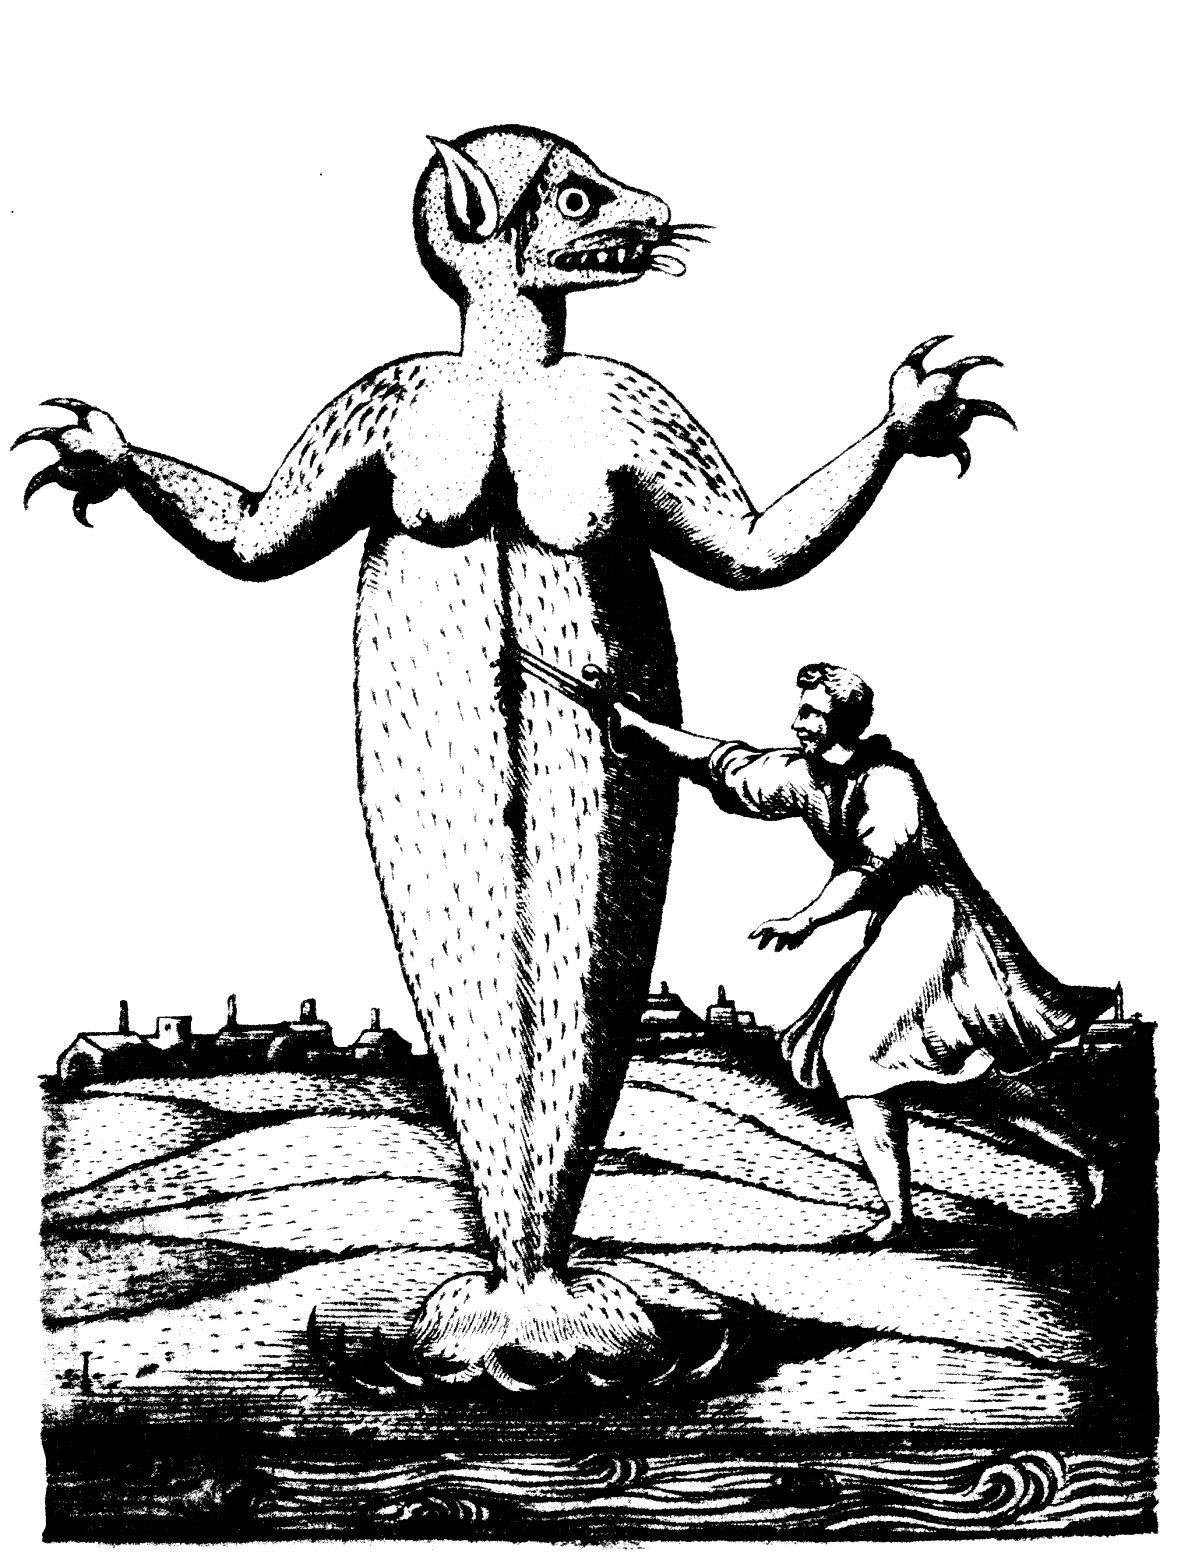
\includegraphics[width=9cm]{1.png}\index{monstro marinho|ii}
\end{figure}

\chapter[Do gentio]{do gentio\subtitulo{que há nesta província, da
condição\break e costumes dele, e de como se governam na paz}} 
\hedramarkboth{do gentio}{gandavo}
										\index{gentios|(}%

\noindent\textsc{Já que tratamos} da terra, e das coisas que nela foram criadas para o
homem, razão parece que demos aqui notícia dos naturais dela; a qual
posto que não seja de todos em geral, será especialmente daqueles que
habitam pela costa, e em partes pelo sertão dentro muitas léguas com
que temos comunicação. Os quais ainda que estejam divisos, e haja entre
eles diversos nomes de nações, todavia na semelhança, condição,
costumes, e ritos gentílicos todos são uns. E se em alguma maneira diferem
nesta parte, é tão pouco, que se não pode fazer caso disso, nem
particularizar coisas semelhantes, entre outras mais notáveis, que
todos geralmente seguem como logo adiante direi.

Estes índios são de cor baça 								\index{gentios!descrição}%
e cabelo corredio; têm o rosto amassado e
algumas feições dele à maneira de chins. Pela maior parte são bem
dispostos, rijos e de boa estatura. Gente mui esforçada e que estima
pouco morrer, temerária na guerra e de muito pouca consideração. São
desagradecidos em grã maneira, e mui desumanos e cruéis, inclinados a
pelejar e vingativos por extremo. Vivem todos mui descansados sem terem
outros pensamentos, senão de comer, beber, e matar gente, e por isso
engordam muito. Mas com qualquer desgosto pelo conseguinte tornam a
emagrecer.
E muitas vezes pode neles tanto a imaginação, que se algum
deseja a morte, ou alguém lhes mete em cabeça que há de morrer tal dia,
ou tal noite, não passa daquele termo que não morra. São mui
inconstantes e mudáveis. Crêem de ligeiro tudo aquilo que lhes persuadem
por dificultoso e impossível que seja, e com qualquer dissuasão
facilmente o tornam logo a negar. São mui desonestos e dados à
sensualidade, e assim se entregam aos vícios como se neles não houvera
razão de homens. Ainda que todavia em seu ajuntamento os machos com as
fêmeas têm o devido resguardo, e nisto mostram ter alguma vergonha.
A língua de que usam toda pela costa é uma, ainda que em certos			\index{gentios!língua}%
vocábulos difere em algumas partes. Mas não de maneira que se deixem uns
aos outros de entender, e isto até altura de 27 graus, que
daí por diante, há outra gentilidade de que nós não temos tanta
notícia, que falam já outra língua diferente. Esta \mbox{de que} trato que é
geral pela costa, é mui branda, e a qualquer nação fácil de tomar.
Alguns vocábulos há nela de que não usam senão as fêmeas, e outros que não servem
senão para os machos. Carece de três letras, convém a saber, não se		\index{fe, lei, rei@fé, lei, rei}%
acha nela, \textit{f}, nem, \textit{l}, nem, \textit{r},\footnote{ Lugar comum sobre o indígena sem Fé, Lei
ou Rei, também presente na Carta de Caminha, e em outras crônicas e sermões entre
tantas outras espécies de discursos, utilizada para legitimar o jugo da coroa
portuguesa promovido por colonos, historiadores, jesuítas etc.} coisa digna de
espanto, porque assim não têm  \label{feleirei}%
Fé, nem Lei, nem Rei. E desta maneira vivem desordenadamente sem terem		\index{gentios!fé, lei, rei}%
além disto conta, nem peso, nem medido. Não adoram a coisa alguma, nem
têm para si que há depois da morte glória para os bons, e pena para os		\index{gentios!imortalidade da alma}%
maus. E o que sentem da imortalidade d'alma não é mais que terem para
si que seus defuntos andam na outra vida feridos, despedaçados, ou de
qualquer maneira que acabaram nesta. E quando algum morre, costumam
enterrá{}-lo em uma cova assentado sobre os pés com sua rede às costas que
em vida lhe servia de cama. E logo pelos primeiros dias põem{}-lhe seus
parentes de comer em cima da cova, e também alguns lho costumam a
meter dentro quando o enterram, e totalmente cuidam que comem, e dormem
na rede que têm consigo na mesma cova. Esta gente não tem entre si nenhum rei nem outro gênero de justiça, senão um
principal em cada aldeia, que é como capitão, ao qual obedecem por
vontade e não por força. Quando este morre fica seu filho no mesmo
lugar por sucessão, e não serve de outra coisa senão de ir com eles à
guerra e aconselhá{}-los como se hão de haver na peleja. Mas não castiga
seus erros, nem manda sobre eles coisa alguma contra suas vontades. E
assim a guerra, que agora têm uns contra outros, não se levantou na terra
 por serem diferentes em leis nem em costumes, nem por cobiça alguma de
interesse, mas porque antigamente se algum acertava de matar outro,		\index{gentios!guerras entre bandos}%
como ainda agora algumas vezes acontece (como eles sejam vingativos e
vivam como digo absolutamente sem terem superior algum a que obedeçam
nem temam) os parentes do morto se conjuravam contra o matador e sua
geração e se perseguiam com tão mortal ódio uns a outros, que daqui
veio dividirem{}-se em diversos bandos, e ficarem inimigos da maneira que
agora estão. E porque estas dissensões não fossem tanto por
diante, determinaram atalhar a isto usando do remédio seguinte, para
por esta via se poderem melhor conservar na paz e se fazerem mais
fortes contra seus inimigos. E é que quando o tal caso acontece de um
matar a outro, os mesmos parentes do matador fazem justiça dele, e logo		\index{gentios!justiça}%
à vista de todos o afogam. E com isto os da parte do morto ficam
satisfeitos, e uns e outros permanecem em suas amizades como dantes.
Porém como esta lei seja voluntária e executada sem rigor, nem
obrigação de justiça alguma, não querem alguns estar por ela, e daqui
vêm logo pelo mesmo caso a dividirem{}-se, e levantarem{}-se de parte a
parte uns contra os outros como já disse.

As povoações destes índios, são aldeias. Cada uma delas tem sete, oito		\index{aldeias}\index{gentios!aldeias}\index{edificações}%
casas, as quais são mui compridas, feitas à maneira de cordoarias ou
tarracenas, fabricadas somente de madeira, e cobertas com palma ou com
outras ervas do mato semelhantes. Estão todas cheias de gente de uma
parte e de outra, e cada um por si tem sua estância e sua rede armada em
que dorme. E assim estão uns juntos dos outros por ordem, e pelo meio da
casa fica um caminho aberto por onde todos se servem como dormitório,
ou coxia de galé. Em cada casa destas vivem todos muito conformes, sem
haver nunca entre eles nenhumas diferenças. Antes são tão amigos uns dos
outros, que o que é de um é de todos, e sempre de qualquer coisa que um
coma por pequena que seja todos os circunstantes hão de participar\mbox{ dela.}

Quando alguém os vai visitar a suas aldeias, depois que se assenta,			\index{gentios!cantos cerimoniais}%
costumam chegarem{}-se a ele algumas moças escabeladas, e recebem{}-no com
grande pranto derramando muitas lágrimas, perguntando{}-lhe (se é seu
natural) onde andou, que trabalhos foram os que passou depois que daí
se foi, trazendo{}-lhe à memória muitos desastres que lhe puderam
acontecer, buscando enfim para isto as mais tristes e sentidas palavras
que podem achar, para provocarem o choro. E se é português, maldizem a			\index{portugueses}%
pouca dita de seus defuntos pois foram tão mal afortunados que não
alcançaram ver gente tão valorosa e luzida como são os \indice{portugueses}, de
cuja terra todas as boas coisas lhes vêm nomeando algumas que eles têm
em muita estima. E este recebimento que digo é tão usado entre eles,
que nunca ou de maravilha deixam de o fazer, salvo quando
reinam alguma malícia contra os que vão visitar, e lhes querem
fazer alguma traição.

As invenções e galantarias de que usam são trazerem alguns o beiço			\index{gentios!adornos}%
de baixo furado, e uma pedra comprida metida no buraco. Outros há que
trazem o rosto todo cheio de buracos e de pedras, e assim parecem mui
feios e disformes. E isto lhes fazem enquanto são mínimos. Também
costumam todos arrancarem a barba, e não consentem nenhum cabelo em
parte alguma de seu corpo, salvo na cabeça, ainda que ao redor dela por
baixo tudo arrancam. As fêmeas prezam{}-se muito de seus cabelos, e
trazem{}-nos mui compridos, limpos e penteados, e as mais delas, 
enastrados. E assim também machos como fêmeas costumam tingir{}-se algumas
vezes com o sumo de um certo pomo que se chama \indice{jenipapo}, que é verde
quando se pisa, e depois que o põem no corpo e se enxuga, fica mui
negro, e por muito que se lave, não se tira senão aos nove dias. 

As mulheres com que costumam casar são suas sobrinhas, filhas de seus			\index{gentios!laços de parentesco, casamentos, poligamia}%
irmãos, ou irmãs. Estas têm por legítimas e verdadeiras mulheres, e não
lhas podem negar seus pais, nem outra pessoa alguma pode casar com elas,
senão os tios. Não fazem nenhumas cerimônias em seus casamentos, nem
usam de mais neste ato, que de levar cada um sua mulher para si como			\index{casamentos|see{gentios}}%
chega a uma certa idade por que esperam, que serão então de 14 ou			\index{laços de parentesco|see{gentios}}%
15 anos pouco mais ou menos. Alguns deles têm três, quatro mulheres,
a primeira têm em muita estima e fazem dela mais caso que das outras. E			\index{poligamia|see{gentios}}%
isto pela mor parte se acha nos principais, que o tem por estado e por
honra, e prezam{}-se muito de se diferençarem nisto dos outros.

Algumas índias há também entre eles que determinam de ser castas, as
quais não conhecem homem algum de nenhuma qualidade, nem o consentirão
ainda que por isso as matem. Estas deixam todo o exercício de mulheres
e imitam os homens e seguem seus ofícios como se não fossem fêmeas.
Trazem os cabelos cortados da mesma maneira que os machos, e vão à
guerra com seus arcos e flechas e à caça perseverando sempre na				\index{gentios!castidade}%
companhia dos homens, e cada uma tem mulher que a serve com que diz que
é casada, e assim se comunicam e conversam como marido e mulher.

Todas as outras índias quando parem, a primeira coisa que fazem depois
do parto, lavam{}-se todas em uma ribeira, e ficam também dispostas como		\index{gentios!partos}%
se não pariram, e o mesmo fazem à criança que parem. Em lugar delas se
deitam seus maridos nas redes, e assim os visitam e curam como se eles
fossem as mesmas paridas. Isto nasce de elas terem em muita conta os
pais de seus filhos e desejarem em extremo depois que parem deles de em
tudo lhes comprazer.\footnote{ Pode{}-se supor que as descrições dos gentios,
bárbaros, indígenas são produzidas a partir de elementos reconhecíveis
pelo destinatário do texto, em geral, os tidos por melhores na corte portuguesa
no século \textsc{xvi}. Desse modo, como propõe Menandro e outros, lidos em chave
cristã, louva-se o modo de estabelecer o senhorio da coroa evidenciando a
barbárie dos naturais da terra que, em oposição às dignidades e aos costumes dos
que conhecem a doutrina da verdadeira fé, não possuem instituições civis
cristãs, e, por isso, são dignos de serem reduzidos.}

 Todos criam seus filhos viciosamente sem nenhuma maneira de castigo, e			\index{gentios!criação dos filhos}%
mamam até idade de sete, oito anos, se as mães até então não acertam de
parir outros que os tirem das vezes. Não há entre eles nenhumas boas
artes a que se dêem, nem se ocupam noutro exercício, senão em granjear
com seus pais o que hão de comer, debaixo de cujo amparo estão
agasalhados até que cada um por si é capaz de buscar sua vida sem mais
esperarem heranças deles, nem legítimas de que enriqueçam, somente lhes
pagam com aquela criação em que a natureza foi universal a todos os
outros animais que não participam de razão. Mas a vida que buscam, e
granjearia de que todos vivem, é à custa de pouco trabalho e muito mais descansada que a nossa porque não possuem nenhuma fazenda, nem procuram adquiri{}-la como os outros homens, e assim vivem livres de toda cobiça e desejo
desordenado de riquezas, de que as outras nações não carecem; e tanto,
que \indice{ouro} nem \indice{prata} nem pedras preciosas tem entre eles nenhuma valia,		\index{pedraria}%
nem para seu uso têm necessidade de nenhuma coisa destas, nem de outras
semelhantes. Todos andam nus e descalços, assim machos como fêmeas, e
não cobrem parte alguma de seu corpo.\footnote{ Tópica presente 
na Carta de Caminha: ``Ali veríeis galantes, pintados de
preto e vermelho, e quartejados, assim pelos corpos como pelas pernas, que,
certo, assim pareciam bem. Também andavam entre eles quatro ou cinco mulheres,
novas, que assim nuas, não pareciam mal. Entre elas andava uma, com uma coxa, do
joelho até o quadril e a nádega, toda tingida daquela tintura preta; e todo o
resto da sua cor natural''.} 
As camas em que dormem são umas
redes de fio de algodão que as índias tecem num tear feito à sua arte, as		\index{gentios!rede de dormir}%
quais têm nove, dez palmos de comprido, e apanham{}-nas com uns cordéis
que lhe rematam nos cabos em que lhes fazem umas aselhas
de cada banda por onde as penduram de uma parte e de outra, e assim
ficam dois palmos, pouco mais ou menos suspendidas do chão, de maneira
que lhes possam fazer fogo debaixo para se aquentarem de noite, ou
quando lhes for necessário. Os mantimentos que plantam em suas roças			\index{gentios!roças}%
com que se sustentam são aqueles de que atrás fiz menção supra
\indice{mandioca} e \indice{milho zaburro}. Além disto ajudam{}-se da carne de muitos	\index{carnes}%
animais que matam, assim com flechas como por indústria de seus laços e
fojos, onde costumam caçar a mor parte deles. Também se sustentam do
muito marisco e peixes que vão pescar pela costa em \indice{jangadas}, que são		\index{pescaria, técnicas de}\index{caça}%
uns três ou quatro paus pegados nos outros e juntos, de modo que ficam
à maneira dos dedos de uma mão estendida, sobre os quais podem ir duas
ou três pessoas, ou mais se mais forem os paus, porque são mui leves e
sofrem muito peso em cima d'água. Têm quatorze, ou
quinze palmos de comprimento, e de grossura ao redor ocuparão dois, pouco
mais ou menos. Desta maneira vivem todos estes índios sem mais terem			\index{indios@índios}%
outras fazendas entre si, nem granjearias em que se desvelem, nem tampouco
estados nem opiniões de honra, nem pompas para que as hajam
mister. Porque todos (como digo) são iguais, e em tudo tão conformes
nas condições, que ainda nesta parte vivem justamente e conforme à lei		\index{lei da natureza|see{gentios}}\index{gentios!lei da natureza}%
de natureza.\footnote{ Essa interpretação acerca da natureza do
gentio da América reitera interesses de colonos portugueses querelantes,
empenhados em escravizar os indígenas da terra; essa tese, entendida como
murmuração do reino, é contrária à Bula papal de 1537 que decreta os gentios do
Novo Mundo como possuidores de alma, ``ou seja, eram gente como os católicos e
que era vedado escravizá{}-los'' (João A.~Hansen, ``A servidão natural do selvagem e a guerra
justa contra o bárbaro'', em Adauto Novais (org.), \textit{A descoberta do homem e do mundo}, 1998, p.~354.
O autor lembra ainda que esta mesma tese é validada no
Concílio de Trento em 1550 e é contra ela que se bate a Companhia de Jesus.).} 		\index{gentios|)}%


\chapter[Das guerras]{das guerras\subtitulo{que têm uns com
outros\break e a maneira de como se hão nelas}}						 \index{guerras}\index{gentios!guerras} 
\hedramarkboth{das guerras}{gandavo}

\noindent\textsc{Estes índios} têm sempre grandes guerras uns contra os outros e assim	\index{indios@índios}%
nunca se acha neles paz, nem será possível (segundo são vingativos e
odiosos) vedarem{}-se entre eles estas discórdias por outra nenhuma via,
se não for por meios da \indice{doutrina cristã} com que os padres da Companhia		\index{Companhia de Jesus}%
pouco a pouco os vão amansando como adiante direi. As armas com que
pelejam são arcos e flechas, nas quais andam tão exercitados que  de			\index{gentios!missões}%
maravilha erram a coisa que apontem por difícil que seja de acertar. E no
despedir delas são mui ligeiros em extremo, e sobre tudo mui arriscados
nos perigos e atrevidos em grã maneira contra seus adversários. Quando
vão à guerra sempre lhes parece que têm certa a vitória, e que nenhum
de sua companhia há de morrer, e assim em partindo, dizem, vamos matar
sem mais outro discurso nem consideração, e não cuidam que também podem
ser vencidos. E somente com esta sede de vingança, sem esperanças de
despojos, nem de outro algum interesse que a isso os mova, vão muitas
vezes buscar seus inimigos mui longe, caminhando por serras, matos,
desertos e caminhos mui ásperos. Outros costumam ir por mar de umas
terras para outras em umas embarcações a que chamam \indice{canoas} quando querem
fazer saltos ao longo da costa. Estas canoas são feitas à maneira de
lançadeiras de tear de um só pau, em cada uma das quais vão 20, 30
remeiros. Além destas há outras que são da casca de um pau do mesmo
tamanho, que se acomodam muito às ondas, e são mui ligeiras, ainda que
menos seguras, porque se se alagam vão{}-se ao fundo o que não têm as de
pau, que de qualquer maneira sempre andam em cima
d'água. E quando acontece alagar{}-se alguma os mesmos
índios, se lançam ao mar, e a sustentam até que a acabam de esgotar, e			\index{indios@índios}%
outra vez se embarcam nela e tornam a fazer sua viagem.

Todos em seus combates são determinados, e pelejam mui animosamente sem
nenhumas armas defensivas; e assim parece coisa estranha ver dois, três
mil homens nus de parte a parte flechar uns aos outros com grandes
assovios e grita, meneando{}-se  todos com grande ligeireza, de uma parte
para a outra, para que não possam os inimigos apontar nem fazer tiro em
pessoa certa. Porém pelejam desordenadamente, e desmandam{}-se muito uns
e outros em semelhantes brigas, porque não têm capitão que os governe,
nem outros oficiais de guerra, a que hajam de obedecer nos tais tempos.
Mas ainda que desta ordenança careçam, todavia por outra parte, dão{}-se
a grande manha em seus cometimentos, e são mui cautos no escolher do
tempo em que hão de fazer seus assaltos nas aldeias dos inimigos; sobre os
quais costumam dar de noite a hora que os achem mais descuidados. E
quando acontece não poderem logo entrá{}-los por alguma cerca de madeira
lhes ser impedimento que eles têm ao redor da aldeia para sua defensão,			\index{aldeias}%
fazem outra semelhante algum tanto separada da mesma aldeia; e assim a
vão chegando cada noite 10, 12 passos até que um dia amanhece pegada
com a dos contrários, onde muitas vezes se acham tão vizinhos que vêm a
quebrar as cabeças, com paus que arremessam uns aos outros. Mas pela
maior parte os que estão na aldeia ficam melhorados da peleja, e as mais
das vezes se tornam os cometedores desbaratados para suas terras sem
conseguirem vitória, nem triunfarem de seus inimigos, como pretendiam. E
isto assim por não terem armas defensivas nem outros apercebimentos
necessários para se entreterem nos cercos, e fortificarem contra seus
inimigos, como também por seguirem muitos agouros, e qualquer coisa que se lhes
antolha
ser bastante a retirá{}-los de seu intento, e tão
inconstantes e pusilânimes são nesta parte, que muitas vezes com
partirem de suas terras mui determinados. E desejosos de exercitarem
sua crueldade, se acontece encontrar uma certa ave, ou qualquer outra
coisa semelhante que eles tenham por ruim prognóstico, não vão mais por			\index{gentios!maus agouros}%
diante com sua determinação, e dali costumam tornar{}-se outra vez sem
haver algum da companhia que seja contra este parecer. Assim que com
qualquer abusão destas, a todo tempo se abalam mui facilmente, ainda que
estejam mui perto de alcançar vitória, porque já aconteceu terem uma
aldeia quase rendida, e por um papagaio que havia nela falar umas certas		\index{papagaios}%
palavras que lhe eles tinham ensinado, levantaram o cerco e fugiram sem
esperarem o bom sucesso que o tempo lhes prometia, crendo sem dúvida
que se assim o não fizeram, morreram todos a mãos de seus inimigos. Mas
afora esta pusilanimidade a que estão sujeitos, são mui atrevidos (como
digo) e tão confiados em sua valentia, que não há forças de contrários
tão poderosas que os assombrem, nem que os façam desviar de suas
bárbaras e vingativas tenções. A este propósito contarei alguns casos
notáveis que aconteceram entre eles, deixando outros muitos à parte de
que eu pudera fazer um grande volume, se minha tenção fora escrevê{}-los
em particular como cada um dos seguintes.

Na capitania de São Vicente sendo capitão \indiceAB{Jorge}{Ferreira}, aconteceu darem		\index{Sao Vicente@São Vicente}%
os contrários em uma aldeia que estava não mui longe dos \indice{portugueses}, e
neste assalto matarem um filho do principal da mesma aldeia. E porque
ele era bem quisto e amado de todos, não havia pessoa nela que o não
pranteasse, mostrando com lágrimas e palavras magoadas o sentimento de
sua morte. Mas o pai, como corrido e afrontado de não haver ainda neste
caso tomado vingança, pediu a todos com eficácia que se o amavam
dissimulassem a perda de seu filho, e que por nenhuma  via o 
quisessem chorar. Passados três ou quatro meses depois da morte do
filho, mandou aperceber sua gente  como convinha, por lhe parecer
aquele tempo mais favorável e acomodado a seu propósito, o que todos
logo puseram em efeito. E dali a poucos dias deram consigo na terra dos
contrários (que seria distância de três jornadas pouco mais ou menos)
onde fizeram suas ciladas junto da aldeia em parte que mais pudessem
ofender a seus inimigos. E tanto que anoiteceu, o mesmo principal se
apartou da companhia com 10 ou 12 flecheiros escolhidos de que ele
mais se confiava, e com eles entrou na mesma aldeia dos inimigos, que o			\index{gentios!crueldade}%
haviam ofendido. E deixando{}-os à parte, só, sem outra pessoa o seguir,
começou de rodear uma casa e outra espreitando com muita cautela de
maneira que não fosse sentido. E da prática que eles tinham uns com os
outros veio a conhecer pela notícia do nome qual era, e onde estava o
que havia morto seu filho, e para se acabar de satisfazer, chegou{}-se da
banda de fora a sua instância, e como foi bem certificado de ele ser
aquele, deixou{}-se ali estar lançado em terra, esperando que se
aquietasse a gente. E tanto que viu horas acomodadas para fazer a sua,
rompeu a palma mui mansamente, de que a casa estava coberta, e entrando
foi{}-se direito ao matador, ao qual cortou logo a cabeça em breve espaço
com um cutelo que para isso levava. Feito isto tomou{}-a nas mãos e
saiu{}-se fora a seu salvo. Os inimigos que neste tempo acordaram ao
reboliço e estrondo do morto, conhecendo serem contrários, começaram de
os seguir. Mas como seus companheiros que ele havia deixado em guarda
estavam prontos, ao sair da casa mataram muitos deles, e assim se foram
defendendo até chegarem às ciladas, donde todos saíram com grande
ímpeto contra os que os seguiam, e ali mataram muitos mais. E com esta
vitória se vieram recolhendo para sua terra com muito prazer e
contentamento. E o principal que consigo trazia a cabeça do inimigo,
chegando a sua aldeia a primeira coisa que fez foi{}-se ao meio do
terreiro da mesma aldeia e ali a fixou num pau à vista de todos dizendo
estas palavras: ``agora companheiros e amigos meus que eu tenho vingada a
morte de meu filho, e trazida a cabeça do que o matou diante de vossos
olhos, vos dou licença que o choreis, muito em boa hora, que dantes com mais
razão me podereis a mim chorar, enquanto vos parecia que por algum
descuido dilatava esta vingança, ou que por ventura esquecido de tão
grande ofensa já não pretendia tomá{}-la, sendo eu aquele a quem mais
devia tocar o sentimento de sua morte''. Dali por diante foi sempre este
principal mui temido, e ficou seu nome afamado por toda aquela terra.

Outro caso de não menos admiração aconteceu entre \indice{Porto Seguro} e o
\indice{Espírito Santo}, naquelas guerras onde mataram \indiceAB{Fernão de}{Sá}, filho de \indiceAB{Mem
de}{Sá}, que então era governador{}-geral destas partes. E foi que tendo os
\indice{portugueses} rendida uma aldeia com favor de alguns índios nossos amigos que
tinham de sua parte, chegaram a uma casa para fazerem presa nos inimigos
como já tinham feito em cada uma das outras. Mas eles, deliberados a
morrer, não consentiram que nenhum entrasse dentro; e os de fora vendo
sua determinação, e que por nenhuma via se queriam entregar,
disseram{}-lhes que se logo a hora o não faziam, lhes haviam de pôr fogo à
casa sem nenhuma remissão. E vendo os nossos que com eles não
aproveitava este desengano, antes se punham de dentro em determinação
de matar quantos pudessem, lhes puseram fogo. E estando a casa assim
ardendo, o principal deles vendo que já não tinham nenhum remédio de			\index{gentios!vingança}%
salvação nem de vingança, e que todos começavam de arder, remeteu de
dentro com grande fúria a outro principal dos contrários que passava
por defronte da porta da banda de fora, e de tal maneira o abarcou, que
sem se poder livrar de suas mãos, o meteu consigo em casa e no mesmo
instante se lançou com ele na fogueira, onde arderam ambos com os mais
que lá estavam sem escapar nenhum.

Neste mesmo tempo e lugar deu um português uma tão grã cutilada a um
índio, que quase o cortou pelo meio, o qual caindo no chão já como			
morto, antes que acabasse de expirar, lançou a mão a uma palha que achou
diante de si, e atirou com ela ao que o matara, como que se dissera: ``recebe{}-me 
a vontade que te não posso mais fazer que isto que te faço em
sinal de vingança''. Donde verdadeiramente se pode inferir que outra
nenhuma coisa os atormenta mais na hora de sua morte que a mágoa 
que levam de se não poderem vingar de seus inimigos.
%Ilustração p.~80 do pdf.

\chapter[Da morte que dão aos cativos]{da morte que\break dão aos cativos\subtitulo{e crueldades que usam com eles}} 
\hedramarkboth{da morte que dão aos cativos}{gandavo}

\noindent\textsc{Uma das coisas} em que estes índios mais repugnam o ser da natureza
humana, e em que totalmente parece que se extremam dos outros homens, é
nas grandes e excessivas crueldades que executam em qualquer pessoa que
podem haver às mãos, como não seja de seu rebanho. Porque não tão
somente lhe dão cruel morte em tempo que mais livres e desimpedidos
estão de toda a paixão, mas ainda depois disso, por se acabarem de			\index{canibalismo|(}\index{gentios!crueldade}%
satisfazer lhe comem todos a carne, usando nesta parte de cruezas tão			\index{gentios!canibalismo|(}%
diabólicas, que ainda nelas excedem aos brutos animais que não têm uso
de razão, nem foram nascidos para obrar clemência. 

Primeiramente quando tomam algum contrário, se logo naquele flagrante o
não matam, levam{}-no a suas terras para que mais a seu sabor se possam
todos vingar dele. E tanto que a gente da aldeia tem notícia que eles
trazem o cativo, daí lhe vão fazendo um caminho até obra de meia légua,
pouco mais ou menos, onde o esperam. Ao qual em chegando, recebem todos
com grandes afrontas e vitupérios, tangendo{}-lhe umas flautas que
costumam fazer das canas das pernas de outros contrários semelhantes que
matam da mesma maneira. E como entram na aldeia depois de assim andarem
com ele triunfando de uma parte para outra, lançando{}-lhe ao pescoço uma
corda de algodão que para isso têm feita, a qual é mui grossa, quanto
naquela parte que o abrange, e tecida ou enlaçada de maneira que
ninguém a pode abrir nem cerrar senão é o mesmo oficial que a faz. Esta
corda tem duas pontas compridas por onde o atam de noite para não
fugir. Dali o metem numa casa, e junto da estância daquele que o cativou
lhe armam uma rede, e tanto que nela se lança, cessam todos os agravos
sem haver mais pessoa que lhe faça nenhuma ofensa. E a primeira coisa
que logo lhe apresentam é uma moça a mais formosa e honrada que há na
aldeia, a qual lhe dão por mulher, e daí por diante ela tem cargo de lhe
dar de comer e de o guardar, e assim não vai nunca para parte que o não
acompanhe. E depois de o terem desta maneira mui regalado um ano, ou o
tempo que querem, determinam de o matar e aqueles últimos dias antes
de sua morte, por festejarem a execução desta vingança, aparelham muita
louça nova, e fazem muitos vinhos do sumo de uma planta, que se chama
\indice{aipim}, de que atrás fiz menção. Neste mesmo tempo lhe ordenam uma casa
nova onde o metem. E o dia que há de padecer, pela manhã muito cedo
antes que o sol saia, o tiram dela, e com grandes cantares e folias, o
levam a banhar a uma ribeira. E tanto que o tornam a trazer vão{}-se com
ele a um terreiro que está no meio da aldeia e ali lhe mudam aquela
corda do pescoço à cinta, passando{}-lhe uma ponta para trás, outra para
diante. E em cada uma delas pegados dois, três índios. As mãos lhe deixam
soltas porque folgam de o ver defender com elas; e assim lhe chegam uns
pomos duros que têm entre si à maneira de laranjas com que possa atirar
e ofender a quem quiser. E aquele que está deputado para o matar é um
dos mais valentes e honrados da terra, a quem por favor e
preeminência de honra concedem este ofício. O qual se empena primeiro por todo o corpo
com penas de \indice{papagaios} e de outras aves de várias cores.  E assim sai
desta maneira com um índio que lhe traz a espada sobre um alguidar, a
qual é um pau mui duro e pesado, feita a maneira de uma maça, ainda que
na ponta tem alguma semelhança de pá. E chegando ao padecente a toma nas
mãos, e lha passa por baixo das pernas e dos braços meneando{}-a de uma
parte para outra. Feitas estas cerimônias, afasta{}-se algum tanto dele, e
começa de lhe fazer uma fala a modo de pregação, dizendo{}-lhe que se
mostre mui esforçado em defender sua pessoa, para que o não desonre,
nem digam que matou um homem fraco, afeminado e de pouco ânimo, e que
se lembre que dos valentes é morrerem daquela maneira em mãos de seus
inimigos, e não em suas redes como mulheres fracas, que não foram
nascidas para com suas mortes ganharem semelhantes honras. E se o
padecente é homem animoso, e não está desmaiado naquele passo (como
acontece a alguns), responde{}-lhe com muita soberba e ousadia, que o mate
muito embora, porque o mesmo tem ele feito a muitos seus parentes e
amigos. Porém que lhe lembre que assim como tomam de suas mortes
vingança nele, que assim também os seus o hão de vingar como valentes
homens, e haverem{}-se ainda com ele e com toda sua geração daquela mesma
maneira. Ditas estas e outras palavras semelhantes, que eles costumam
arrazoar nos tais tempos, remete o matador a ele com a espada levantada
nas mãos, em postura de o matar, e com ela o ameaça muitas vezes,
fingindo que lhe quer dar. O miserável padecente que sobre si vê a
cruel espada entregue naquelas violentas e rigorosas mãos do capital
inimigo, com os olhos e sentidos prontos nela, em vão se defende quanto
pode. E andando assim nestes cometimentos, acontece algumas vezes virem a
braços, e o padecente tratar mal ao matador com a mesma espada. Mas
isto raramente, porque acodem logo com muita presteza os circunstantes
a livrá{}-lo de suas mãos. E tanto que o matador vê tempo oportuno, tal
pancada lhe dá na cabeça, que logo lha faz em pedaços. Está uma índia
velha prestes com um cabaço grande na mão, e como ele cai, acode muito
depressa a meter{}-lho na cabeça para tomar nele os miolos e o sangue. E
como desta maneira o acabam de matar, fazem{}-no em pedaços, e cada
principal que aí se acha leva seu quinhão para convidar a gente de sua
aldeia. Tudo enfim assam e cozem, e não fica dele coisa que não comam
todos quantos há na terra. Salvo aquele que o matou não come dele nada,
e além disso manda{}-se sarjar por todo o corpo, porque tem por certo que
logo morrerá, se não derramar de si aquele sangue tanto que acaba de
fazer seu ofício. Algum braço ou perna, ou outro qualquer pedaço de
carne costumam assar no fumo, e tê{}-lo guardado alguns meses, para
depois quando o quiserem comer, fazerem novas festas, e com as mesmas
cerimônias tornarem a renovar outra vez o gosto desta vingança como no
dia em que o mataram. E depois que assim chegam a comer a carne de seus
contrários, ficam os ódios confirmados perpetuamente, porque sentem
muito esta injúria, e por isso andam sempre a vingar{}-se uns dos outros
como já tenho dito. E se a mulher que foi do cativo acerta de ficar
prenhe, aquela criança que pare, depois de criada, matam{}-na e comem{}-na		\index{canibalismo|)}\index{gentios!canibalismo|)}%
sem haver entre eles pessoa alguma que se compadeça de tão injusta
morte. Antes seus próprios avós (a quem mais devia chegar esta mágoa)
são aqueles que com maior gosto o ajudam a comer, e dizem que como
filho de seu pai se vingam dele, tendo para si que em tal caso não toma			\index{gentios!aborto}%
esta criatura nada da mãe, nem crêem que aquela inimiga semente pode ter
mistura com seu sangue. E por este respeito somente lhe dão esta
mulher com que converse, porque na verdade são eles tais, que não se
haveriam de todo ainda por vingados do pai, se no inocente filho não			\index{gentios!casamento misto}%
executassem esta crueldade. Mas porque a mãe sabe o fim que hão de dar
a esta criança, muitas vezes quando se sente prenhe, mata{}-a dentro da
barriga, e faz com que não venha a luz. Também acontece algumas vezes
afeiçoar{}-se tanto ao marido, que chega a fugir com ele para sua terra
pelo livrar da morte. E assim alguns \indice{portugueses} desta maneira
escaparam, que ainda hoje em dia vivem. Porém o que por esta via se não
salva, ou por outra qualquer manha oculta, será coisa impossível
escapar de suas mãos com vida, porque não costumam dá{}-la a nenhum
cativo, nem desistirão da vingança que esperam tomar dele por nenhuma
riqueza do mundo, quer seja macho, quer fêmea. Salvo se o principal, ou
outro qualquer da aldeia acerta de casar com alguma escrava sua contrária
(como muitas vezes acontece) pelo mesmo caso fica libertada, e assentam
em não pretenderem vingança dela, por comprazerem àquele que a tomou
por mulher. Mas tanto que morre de sua morte natural, por cumprirem as
leis de sua crueldade (havendo que já nisto não ofendem ao marido)
costumam quebrar{}-lhe a cabeça, ainda que isto raras vezes, porque se
tem filhos não deixam chegar ninguém a ela, e estão guardando seu corpo
até que o dêem à sepultura.

Outros índios de outra nação diferente se acham nestas partes, ainda mais
ferozes e de menos razão que estes. Chamam{}-se \indice{aimorés},\footnote{ O
termo \textit{aimoré}, provavelmente, tornou-se conhecido 
dos portugueses por intermédio dos tupinambás e seria referência a algum grupo que
habitava também a região do \textsc{ne}. Era comum
pensar que os aimorés eram botocudos. [N.~do E.]}
os quais andam									\index{gentios!aimorés}%
por esta costa como salteadores, e habitam da capitania dos \indicex{Ilhéus}{Ilheus} até
a de \indiceAB{Porto}{Seguro}, aonde vieram ter do sertão no ano de [15]55, pouco mais
ou menos. A causa de residirem nesta parte mais que nas outras é por
serem aqui as terras mais acomodadas a seu propósito, assim pelos
grandes matos que têm onde sempre andam emboscados, como pela muita
\indice{caça} que há nelas, que é o seu principal mantimento de que se
sustentam. Estes aimorés são mais alvos e de maior estatura que os
outros índios da terra, com a língua dos quais não tem a destes nenhuma			\index{indios@índios}\index{gentios!língua}%
semelhança nem parentesco. Vivem todos entre os matos como brutos
animais, sem terem povoações nem casas em que se recolham. São mui
forçosos em extremo, e trazem uns arcos mui compridos e grossos
conformes a suas forças, e as flechas da mesma maneira. Estes alarves
têm feito muito dano nestas capitanias depois que desceram a esta
costa, e mortos alguns \indice{portugueses} e \indice{escravos}, porque são mui \indice{bárbaros},
e toda a gente da terra lhes é odiosa. Não pelejam em campo, nem têm
ânimo para isso. Põem{}-se entre o mato junto de algum caminho, e tanto
que alguém passa, atiram{}-lhe ao coração, ou à parte onde o matem, e não
despedem flecha que não na empreguem. As mulheres trazem uns paus
grossos à maneira de maças com que os ajudam a matar algumas pessoas
quando se oferece ocasião. Até agora não se pôde achar nenhum remédio
para destruir esta pérfida gente, porque tanto que vem tempo oportuno,
fazem seus saltos, e logo se recolhem ao mato mui depressa, onde são
tão ligeiros e manhosos, que quando cuidamos que vão fugindo ante quem
os persegue, então ficam atrás escondidos atirando aos que passam
descuidados, e desta maneira matam muita gente. Pela qual razão todos
quantos \indice{portugueses} e índios há na terra os temem muito, e assim onde os 	\index{indios@índios}%
há, nenhum morador vai a sua fazenda por terra, que não leve consigo
quinze vinte escravos de arcos e flechas para sua defensão. O mais do
tempo andam derramados por diversas partes, e quando se querem ajuntar
assoviam como pássaros, ou como \indice{bugios}, de maneira que uns aos outros
se entendem e conhecem, sem serem da outra gente conhecidos. Não dão
vida uma só hora a ninguém, porque são mui repentinos e acelerados no
tomar de suas vinganças, e tanto, que muitas vezes estando a pessoa
viva, lhe cortam a carne, e lha estão assando e comendo à vista de seus \EP[1]
olhos. São finalmente estes \indice{selvagens} tão ásperos e cruéis, que não se
pode com palavras encarecer sua dureza. Alguns deles houveram já os			\index{selvagens|seealso{gentios}}%
\indice{portugueses} às mãos, mas como sejam tão bravos e de condição tão
esquiva nunca os puderam amansar nem submeter a nenhuma servidão, como os		
outros índios da terra que não recusam como estes a sujeição do cativeiro.

Também há uns certos índios junto do \indiceAB{rio do}{Maranhão}, da banda do		\index{indios@índios}%
Oriente em altura de dois graus, pouco mais ou menos, que se chamam
\indice{tapuias},\footnote{É difícil dizer ao certo o que designa a palavra \textit{tapuia},  
pois o termo indicaria apenas aqueles que não falam a mesma língua desses tupinambás. Trata-se de uma
expressão atribuída à forma como os tupinambás se refeririam a outros
grupos falantes de outras línguas. Parece ser um termo genérico para
indicar ``os outros'' e aí estariam referidos principalmente os jê. [N.~do E.]}  
os quais dizem que são da mesma nação destes \indice{aimorés}, ou pelo \index{gentios!aimorés}%
menos irmãos em armas, porque ainda que se encontrem não ofendem uns			\index{gentios!tapuias}%
aos outros. Estes \indice{tapuias} não comem a carne de nenhuns contrários, 
antes são inimigos capitais daqueles que acostumam comer, e os
perseguem com mortal ódio. Porém pelo contrário têm outro rito muito
mais feio e diabólico, contra natureza, e digno de maior espanto. E é,
que quando algum chega a estar doente de maneira que se desconfie de
sua vida, seu pai ou mãe, irmãos, ou irmãs, ou quaisquer outros
parentes mais chegados, o acabam de matar com suas próprias mãos,			\index{gentios!crueldade}%
havendo que usam assim com ele de mais piedade, que consentirem que a
morte o esteja senhoreando e consumindo por termos tão vagarosos. E o
pior que é, que depois disto o assam e cozem e lhe comem toda a carne,
e dizem que não hão de sofrer que coisa tão baixa e vil, como é a
terra, lhes coma o corpo de quem eles tanto amam, e que pois é seu
parente, e entre eles há tanta razão de amor, que sepultura mais
honrada lhe podem dar que metê{}-lo dentro em si e agasalhá{}-lo para			\index{canibalismo}\index{gentios!canibalismo}%
sempre em suas entranhas.

E porque meu intento principal não foi tratar aqui senão daqueles índios
que são gerais pela costa, com que os \indice{portugueses} têm comunicação, não
me quis mais deter em particularizar alguns ritos desta e de outras
nações diferentes que há nesta província, por me parecer que seria
temeridade e falta de consideração escrever em \indice{história} tão verdadeira
coisas em que porventura podia haver falsas informações, pela pouca \EP[1]
notícia que ainda temos da mais gentilidade que habita pela terra dentro.		\index{gentios}%	

\chapter[Do fruto que fazem nestas partes os padres]{do fruto que
fazem\break nestas partes os padres\subtitulo{da Companhia com sua
doutrina}} 
\hedramarkboth{do fruto que fazem nestas partes os padres}{gandavo}

\noindent\textsc{Por todas} as capitanias desta província estão edificados mosteiros dos
padres da Companhia de Jesus, e feitas em algumas partes algumas igrejas
entre os índios que são de paz, onde residem alguns padres para os			\index{gentios!de paz}%
doutrinar e fazer cristãos, o que todos aceitam facilmente sem				\index{Companhia de Jesus}%
contradição alguma. Porque como eles não tenham nenhuma lei, nem coisa			\index{conversão dos gentios}%
entre si a que adorem, é{}-lhes muito fácil tomar esta nossa. E assim			\index{gentios!conversão dos}%
também com a mesma facilidade por qualquer coisa leve a tornam a
deixar, e muitos fogem para o sertão, depois de batizados e instruídos
na \indice{doutrina cristã}. E porque os padres vêem a inconstância que há
neles, e a pouca capacidade que têm para observarem os \indice{mandamentos} da
lei de \indice{Deus} (principalmente os mais antigos, que são aqueles em que
menos frutifica a semente de sua doutrina), procuram em especial
plantá{}-la em seus filhos, os quais levam de meninos instruídos nela. E
desta maneira se tem esperança (mediante a divina graça) que pelo tempo
adiante se vá edificando a religião cristã por toda esta província, e
que ainda nela floresça universalmente a nossa santa fé católica, como
noutra qualquer parte da cristandade. E para que o fruto desta
doutrina se não perdesse, antes de cada vez fosse em mais crescimento,
determinaram os mesmos padres de atalhar todas as ocasiões que lhe
podiam da nossa parte ser impedimento, causa de escândalo, e prejuízo
às consciências dos moradores da terra. Porque como estes índios		\index{indios@índios}%
cobiçam muito algumas coisas que vão deste reino, convém a saber,
camisas, pelotes, ferramentas, e outras peças semelhantes, vendiam{}-se a	\index{gentios!escambo}%
troco delas uns aos outros aos \indice{portugueses}; os quais a voltas disto
salteavam quantos queriam, e faziam{}-lhes muitos agravos sem ninguém
lhes ir à mão. Mas já agora não há esta desordem na terra nem resgastes
como soía. Porque depois que os padres viram a sem razão que com eles
se usava, e o pouco serviço de \indice{Deus} que daqui se seguia, proveram neste
negócio e vedaram (como digo) muitos saltos que faziam os mesmos
\indice{portugueses} por esta costa; os quais encarregavam muito suas
consciências com cativarem muitos índios contra direito, e moverem{}-lhes
\indice{guerras injustas}.\footnote{ Não se trata de imparcialidade do
historiador português, mas de revelar ao soberano publicamente que
súditos seus foram responsáveis por maus atos, tornando pesadas suas
consciências particulares (que os conduzirá ao Inferno), mas
principalmente corrompendo o corpo do Império. A função jurídica do rei
o faz auditório{}-juiz deste relato, isto é, do discurso público do
historiador a respeito de maus feitos nas províncias do reino. Aqui já
se executam as \textit{leis do reino}, que então eram provavelmente o
objeto principal do zelo de qualquer historiador, que não serve senão
por lhe conservar a memória, à lei do rei e à fé cristã.} E para evitar tudo
isto, ordenaram os padres, e fizeram com os \indice{governadores} e \indice{capitães} da
terra, que não houvessem mais resgates daquela maneira, nem
consentissem que fosse nenhum português a suas \indice{aldeias} sem licença do
seu mesmo capitão. E se algum faz o contrário, ou os agrava por
qualquer via que seja, ainda que vá com licença, pelo mesmo caso é mui
bem castigado, conforme a sua culpa. Além disto, para que nesta parte
haja mais \indice{desengano}, quantos \indice{escravos} agora vêm novamente do sertão, ou
de umas capitanias para outras, todos levam primeiro à \indice{alfândega}, e ali
os examinam e lhes fazem perguntas, quem os vendeu, ou como foram
resgatados; porque ninguém os pode vender senão seus pais (se for ainda
com extrema necessidade) ou aqueles que em justa guerra os cativam; e
os que acham mal adquiridos põem{}-nos em sua liberdade. E desta maneira
quantos índios se compram são bem resgatados, e os moradores da terra			\index{indios@índios}%
não deixam por isso de ir muito avante com suas fazendas.

Outros muitos benefícios e obras pias têm feito estes padres e fazem			\index{Companhia de Jesus!benefícios e obras pias}%
hoje em dia nestas partes, a que com verdade se não pode negar muito
louvor. E porque elas são tais que por si apregoam pela terra, não me
quis intermeter a tratá{}-las aqui mais por excesso; basta sabermos quão
aprovadas são em toda parte suas obras por santas e boas, e que sua
tenção não é outra senão dedicá{}-las a nosso Senhor, de quem somente
esperam a gratificação e prêmio de suas virtudes.

\chapter[Das grandes riquezas]{das grandes riquezas\subtitulo{que se esperam da terra do sertão}} 
\hedramarkboth{das grandes riquezas}{gandavo}

\noindent\textsc{Esta província} Santa Cruz, além de ser tão fértil como digo, e abastada	\index{Santa Cruz, província}%
de todos os mantimentos necessários para a vida do homem, é certo ser
também mui rica, e haver nela muito \indice{ouro} e \indice{pedraria}, de que se têm
grandes esperanças. E a maneira de como isto se veio a denunciar e ter				\index{riquezas da terra}%
por coisa averiguada, foi por via dos índios da terra. Os quais como				\index{indios@índios}%
não tenham fazendas que os detenham em suas pátrias, e seu intento não
seja outro senão buscar sempre terras novas, a fim de lhes parecer que
acharam nelas imortalidade e descanso perpétuo, aconteceu levantarem{}-se
uns poucos de suas terras, e meterem{}-se pelo sertão dentro; onde, depois
de terem entrado algumas jornadas, foram dar com outros índios seus
contrários, e ali tiveram com eles grande guerra. E por serem muitos e
lhes darem nas costas, não se puderam tornar outra vez a suas terras.
Por onde lhes foi forçado entrar pela terra dentro muitas léguas. E
pelo trabalho e má vida que neste caminho passaram, morreram muitos
deles e os que escaparam foram dar em uma terra onde havia algumas povoações
mui grandes e de muitos vizinhos, os quais possuíam tanta riqueza que afirmaram 
haver ruas mui compridas entre eles, nas quais se não fazia outra coisa senão lavrar
peças d'\indice{ouro} e \indice{pedraria}. Aqui se detiveram alguns dias
com estes moradores, os quais vendo{}-lhes algumas ferramentas
que eles levavam consigo, perguntaram{}-lhes de quem as haviam, ou por que
meios lhes vinham ter às mãos. Responderam{}-lhes que uma certa gente
habitava ao longo da costa da banda do Oriente, que tinha barba e outro			\index{gentios!descrição}%
parecer diferente, de que as alcançavam, que são os \indice{portugueses}. Os
mesmos sinais lhes deram estes outros dos castelhanos do \indice{Peru},			\index{castelhanos}%
dizendo{}-lhes que também da outra banda tinha notícia haver gente
semelhante, então lhes deram certas rodelas todas chapadas
d'\indice{ouro}, e esmaltadas de \indice{esmeraldas}; e lhes pediram que
as levassem, para que se acaso fossem ter com eles a suas terras, lhes
dissessem que se a troco daquelas peças e outras semelhantes lhes
queriam levar ferramentas e ter comunicação com eles, o fizessem que			\index{gentios!escambo}%
estavam prestes para os receberem com muito boa vontade. Depois disto
partiram{}-se daí e foram dar em o rio das Amazonas, onde se embarcaram			\index{Amazonas, rio}%
em algumas \indice{canoas} que fizeram; e a cabo de terem navegado por ele acima
dois anos, chegaram à província do \indice{Quito}, terra do \indice{Peru} povoada de
\indice{castelhanos}. Os quais vendo esta nova gente, espantaram{}-se muito, e não
sabiam determinar donde eram, nem a que vinham. Mas logo foram
conhecidos por gentio, da província Santa Cruz de alguns \indice{portugueses}		\index{Santa Cruz, província}\index{gentios}%
que então na mesma terra se acharam. E perguntado por eles a causa de
sua vinda contaram{}-lhes o caso miudamente, fazendo{}-os sabedores de tudo
o que lhes havia sucedido. E isto veio{}-nos à notícia, assim por via
dos \indice{castelhanos} do \indice{Peru}, onde estas rodelas foram vendidas por grande
preço, como pela dos mesmos \indice{portugueses} que lá estavam quando isto
aconteceu, com os quais falaram alguns homens deste reino, pessoas de
autoridade, e dignas de crédito, que testificam ouvirem{}-lhes afirmar
tudo isto por extenso da maneira que digo.  E sabe{}-se de certo que está
toda esta riqueza nas terras da conquista del-Rei de \indice{Portugal}, e mais
perto sem comparação das povoações dos \indice{portugueses} que dos \indice{castelhanos}.
Isto se mostra claramente no pouco tempo que puseram estes índios em		\index{indios@índios}%
chegar a ela e no muito que despenderam em passarem daí ao \indice{Peru}, que
foram dois anos como já disse. Além da certeza que por esta via temos,
há outros muitos índios na terra que também afirmam haver no sertão
muito \indice{ouro}; os quais posto que são gente de pouca fé e verdade,	\index{fe, lei, rei@fé, lei, rei}\index{gentios!fé, lei, rei}%
dá{}-se{}-lhes crédito nesta parte, porque acerca disto os mais deles são
contestes, e falam em diversas partes por uma boca. Principalmente é
pública fama entre eles, que há uma lagoa mui grande no interior da
terra, donde procede o rio de São Francisco, de que já tratei; dentro		\index{Sao Francisco@São Francisco, rio}%
da qual dizem haver algumas ilhas, e nelas edificadas muitas povoações,
e outras ao redor delas mui grandes, onde também há muito \indice{ouro}, e mais
quantidade (segundo se afirma) que em nenhuma outra parte desta
província. Também pela terra dentro, não muito longe do rio da Prata		\index{Prata, rio da}%
descobriram os \indice{castelhanos} uma mina de metal, da qual se tem levado \indice{ouro}
ao \indice{Peru}, e de cada quintal dele dizem que se tirou 570
cruzados, e de outro trezentos e tantos; o demais que dela se tira é
\indice{cobre} infinito. Também descobriram outras minas de umas certas pedras		\index{esmeraldas}\index{pedraria}%
brancas e verdes, e de outras cores diversas; as quais são todas de
cinco, seis quinas cada uma à maneira de diamantes, e também lavradas da		\index{diamantes}%
natureza, como se por indústria humana o foram. Estas pedras nascem em
%Jorge: coco é acentuado?
um vaso como coco, o qual é todo oco com mais de quatrocentas pedras			\index{cocos}%
ao redor, todas inseridas na \indice{pedreira} com as pontas para fora. Alguns
destes pedernais se acham ainda imperfeitos; porque dizem que quando			\index{pedernais}%
são de vez que por si arrebentam, com tanto estrondo, como se
disparasse um exército de \indice{arcabuzes}; e assim acharam muitas, que com a
fúria (segundo dizem) se metem pela terra um e dois estádios. Do preço
delas não trato aqui, porque ao presente o não pude saber, mas sei que
assim destas como de outras há nesta província muitas e mui finas, e
muitos metais, donde se pode conseguir infinita riqueza. A qual			\index{metais}%
permitirá \indice{Deus}, que ainda em nossos dias se descubra toda, para que com
ela se aumente muito a coroa destes reinos; aos quais desta maneira
esperamos (mediante o favor divino) ver muito cedo postos em tão feliz
e próspero estado, que mais se não possa desejar.
\ \\ 
\ \\


\begin{center}
Impresso em Lisboa na Oficina\\
de Antonio Gonçalves.
Ano de 1576.\\
\ \\
\textit{Fim}
\end{center}

\index{indios@índios|seealso{gentios}}%
\index{canibalismo|seealso{gentios}}%
\index{onças|seealso{tigres}}%
}
%\part[{{\def\break{}\titulo}}]{\titulo}
} % fim do AtBeginDocument

% Finais -------------------------------------------------------
\AtEndDocument{%
  \publicidade

\pagebreak\ifodd\thepage\paginabranca\fi

\ifdef{\imagemficha}{\IfFileExists{\imagemficha}{\includegraphics[width=.7\textwidth]{\imagemficha}\par}}{}

\mbox{}\vfill\small\thispagestyle{empty}
\begin{center}
\begin{minipage}{.8\textwidth}
\centering\tiny\noindent{}Adverte-se aos curiosos que se imprimiu este livro \ifdef{\grafica}{na gráfica \grafica}{em nossas oficinas}, 
em \today \ifdef{\papelmiolo}{em papel \papelmiolo}, em tipologia Formular e \tipopadrao{}, com diversos sofwares livres, 
entre eles, Lua\LaTeX, git \& ruby. \ifdef{\RevisionInfo{}}{\par(v.\,\RevisionInfo)}{}\par \begin{center}\normalsize\adforn{64}\end{center}
\end{minipage}
\end{center}
}
